% Secao 4 do artigo do LAB03 (template SBC). Issue #99.
% Uso no Overleaf: % Secao 4 do artigo do LAB03 (template SBC). Issue #99.
% Uso no Overleaf: % Secao 4 do artigo do LAB03 (template SBC). Issue #99.
% Uso no Overleaf: % Secao 4 do artigo do LAB03 (template SBC). Issue #99.
% Uso no Overleaf: \input{discussao} depois de \input{resultados}.
% Os numeros vem das mesmas analises da Secao 3 (entregas/laboratorio-03/sprint-03, RQ91 a RQ98).
% Trechos em \apreencher{...} dependem da RQ06 (issue #93) e da validacao manual (issues #85 a #89).

\providecommand{\apreencher}[1]{\textbf{[a preencher: #1]}}

\section{Discussão}
\label{sec:discussao}

\subsection{Hipóteses e resultados}

A Tabela~\ref{tab:hipoteses} confronta cada hipótese informal da Seção~\ref{sec:hipoteses},
registrada antes da análise, com o que encontramos. Nenhuma faixa prevista foi alterada depois
da análise.

\begin{table}[ht]
\centering
\scriptsize
\caption{Hipóteses (Seção~\ref{sec:hipoteses}) frente aos resultados (Seção~\ref{sec:resultados}).}
\label{tab:hipoteses}
\begin{tabular}{p{0.05\linewidth}p{0.28\linewidth}p{0.40\linewidth}p{0.15\linewidth}}
\hline
 & Previsão & Resultado & Veredito \\
\hline
H1 & Mediana de 0,5 a 1 release/semana; Medium e High; cauda longa; poucos Elite
   & Mediana de 0,48; Medium e High somam 75,7\%; 33 extremos; 1,7\% Elite
   & Confirmada, com a mediana pouco abaixo da faixa \\
H2 & (a) em semanas (Medium ou Low); (b) sistematicamente menor; diferença cresce com o tamanho da release
   & (a) = 10,5 dias, com 60,7\% em Medium ou Low; (b) = 12,1 dias, menor em 177 de 300 repositórios, mas
     sem diferença pareada ($p = 0{,}12$); $\rho = -0{,}30$ com o tamanho
   & Parcial: (a) e o efeito do tamanho sim; (b) menor, não \\
H3 & CFR (a) de 10 a 25\%; (b) de 5 a 15\% e mais variável; $|\rho| < 0{,}3$ entre (a) e (b)
   & (a) = 4,6\%; (b) = 18,8\%, com IQR de 44,7 contra 8,8 pontos; $\rho = 0{,}07$
   & Parcial (2 de 4): variabilidade e correlação sim; níveis, não \\
H4 & Recuperação de 1 hora a 1 dia; cauda longa; censura abaixo de 10\%
   & 2,7 horas; P90 de 24,5 horas e máximo de 560; censura de 0,83\% (24 repositórios com $\geq 10$\%)
   & Confirmada \\
H5 & $\rho$ próximo de zero ou levemente negativo no (b) e próximo de zero no (a)
   & (a) $\rho = 0{,}15$; (b) $\rho = 0{,}40$, ou $-0{,}16$ após a linha de base
   & Parcial: vale, fracamente, no (a); não vale no (b) bruto \\
H6 & Efeitos pequenos a médios; contribuidores, tipo e linguagem associados
   & \apreencher{RQ06 (issue \#93)}
   & Pendente \\
H7 & $\geq 30$\% mudam de classe; $\kappa$ de 0,2 a 0,6; pré-releases e tags inflam a frequência; \textit{lead time} (b) melhora a classe
   & 1 de 6 alternativas com $\geq 30$\% (C7: 35,5\%); $\kappa$ de 0,44 a 0,95; pré-releases e tags só melhoram a classe de frequência; (b) melhora 61 repositórios e piora 66
   & Parcial: depende de qual definição muda \\
\hline
\end{tabular}
\end{table}

\subsection{O que surpreendeu e por quê}

\textbf{A velocidade é o gargalo; a estabilidade quase nunca.} Esperávamos CFR de CI entre 10\% e
25\% e encontramos 4,6\%. Com o corte de Elite em 15\%, 83\% dos repositórios são Elite no CFR (a),
e 85,4\% têm estabilidade alta contra 21,1\% com velocidade alta. O resultado é coerente com o
perfil da amostra, projetos populares com CI madura, mas também com a natureza do proxy: o CFR (a)
mede falha de pipeline, concentrada em um ou dois \textit{workflows} (73,1\% das falhas, na mediana),
e não mede defeito que chega ao usuário. Os cortes DORA vêm de questionários com empresas; aqui o
CFR (a) discrimina pouco, e a classe geral fica presa à frequência e ao \textit{lead time}. Já a
frequência baixa tem uma leitura própria: uma biblioteca que publica uma release por mês não está
``deployando'' nada, e a classe Medium da maioria dos repositórios reflete o ritmo de publicação,
não necessariamente uma entrega lenta.

\textbf{Os dois CFR respondem a perguntas diferentes.} O CFR (b) não ficou abaixo do (a), como
previsto, e a correlação entre eles é desprezível ($\rho = 0{,}07$); 57,2\% dos repositórios mudam de
classe ao trocar um pelo outro. A previsão de que medem fenômenos distintos se confirmou, mas o
nível do (b) é frágil: depende de uma heurística cuja versão v1 deixa de fora 39,2\% das releases
(tags fora do SemVer), e a mediana vai de 18,8\% a 43,5\% conforme a versão
(Seção~\ref{sec:rq03}). Sem o F1 contra o consenso da amostra-ouro (\apreencher{P, R e F1 das versões
da heurística e $\kappa$ de Fleiss entre os avaliadores}), não sabemos qual dessas taxas se aproxima da
taxa real de releases corretivas; por isso reportamos as duas variantes e não escolhemos a mais
favorável a uma hipótese.

\textbf{Mais releases, mais CFR (b), mas por aritmética.} Esperávamos ausência de \textit{trade-off}, em
linha com o DORA. O $\rho$ bruto entre frequência e CFR (b) foi de $0{,}40$, e 40\% dos repositórios de
frequência alta têm CFR (b) Elite ou High, contra 75\% dos de frequência baixa. Lido sem cuidado, isso
sugeriria que publicar mais piora a estabilidade. Mas o CFR (b) conta uma falha quando alguma release
\textit{patch} sai em até 7 dias, e quanto mais releases, maior a chance de isso acontecer ao acaso: a fração
de releases com alguma sucessora em 7 dias tem $\rho = 0{,}83$ com a frequência, enquanto a proporção de
\textit{patches} quase não varia com ela. Embaralhando, em cada repositório, quais releases são corretivas,
o CFR (b) esperado ao acaso tem $\rho = 0{,}59$ com a frequência, acima do observado, e o $\rho$ parcial,
controlando esse esperado, é $-0{,}16$. Para o CFR (a), a relação é fraca ($\rho = 0{,}15$) e perde a
significância ao controlar idade e contribuidores ($0{,}09$; $p = 0{,}14$). Assim, os dados
\textit{open source} não confirmam nem contradizem a afirmação do DORA de que velocidade e estabilidade
andam juntas: o proxy de entrega tem um acoplamento aritmético com a frequência, e o de CI quase não
discrimina. Correlação não implica causalidade; tamanho da equipe, maturidade e automação de
releases podem afetar as duas medidas.

\textbf{\textit{Lead time} por \textit{commit} não é menor que por release.} Previmos o (b) sistematicamente
menor, porque um \textit{commit} antigo ``esquecido'' infla o (a) e é diluído no (b). O mecanismo aparece nas
releases grandes ($\rho = -0{,}30$ entre o tamanho e a razão (b)/(a)), mas o (b) pondera as releases pelo
número de \textit{commits}: onde poucas releases grandes concentram \textit{commits} antigos e muitas releases
pequenas são rápidas, a mediana por \textit{commit} cai dentro das grandes e supera a por release. No
agregado, as variantes divergem em ambos os sentidos, e o teste pareado não as separa.

\textbf{A classificação é frágil, mas não a todas as escolhas.} Dos repositórios classificados em todas as
combinações, 41,6\% mudam de classe em pelo menos uma alternativa, e o efeito não é uniforme: trocar a
unidade de deploy muda de 3,6\% a 10,7\% das classes, sempre para melhor ($\kappa \geq 0{,}85$), enquanto as
combinações com o CFR (b) mudam de 20,8\% a 35,5\%, em geral para pior ($\kappa$ de 0,44 a 0,68). Como o CFR (b) depende de uma heurística
ainda sem F1, parte desse efeito pode ser do proxy, não da definição. As conclusões das RQ01 a RQ05
valem, portanto, para a combinação C1 e são condicionais à definição de falha, e menos à de deploy.

\subsection{Implicações}

Para quem minera métricas DORA no GitHub, três cuidados decorrem dos resultados. Primeiro, release
não é deploy, e falha de CI não é falha em produção; as classes servem para comparar repositórios entre si,
não para dizer que um projeto de código aberto é ``Elite'' no sentido do DORA. Segundo, o CFR
baseado em releases corretivas só tem sentido com uma heurística validada contra julgamento humano, e
deve ser comparado ao que o acaso produziria quando a frequência de releases é alta. Terceiro, vale
reportar a sensibilidade às definições, como fizemos na RQ07, porque a escolha do CFR por si só
reclassifica de 20,8\% a 35,5\% dos repositórios. A RQ06 (características dos repositórios)
ainda não foi analisada (\apreencher{discussão da RQ06 e da H6}); as ameaças à validade que decorrem
destes achados estão na Seção~5.
 depois de % Secao 3 do artigo do LAB03 (template SBC). Issue #99.
% Uso no Overleaf: \input{resultados} depois de \input{metodologia}; as figuras ficam em figuras/
% (\usepackage{graphicx}, ja no template).
%
% Todos os numeros vem das analises do repositorio (entregas/laboratorio-03/sprint-03):
% RQ91 (RQ01), RQ94 (RQ02), RQ97 (RQ03), RQ92 (RQ04), RQ95 (classificacao C1),
% RQ98 (RQ05), RQ96 (RQ07). Janela provisoria; CFR (b) com a heuristica v1, ainda sem F1 medido.
% Trechos em \apreencher{...} dependem de analises ainda nao feitas (RQ06, issue #93) ou da
% validacao manual (issues #85 a #89). Busque por "apreencher" antes de entregar.

\providecommand{\apreencher}[1]{\textbf{[a preencher: #1]}}

\section{Resultados}
\label{sec:resultados}

Os resultados se referem aos 300 repositórios da amostra final (Seção~\ref{sec:funil}),
na janela de 01/10/2025 a 30/09/2026, ainda provisória (Seção~\ref{sec:definicoes}). Cada
repositório tem o mesmo peso e a estatística da amostra é a mediana dos valores dos
repositórios, com o intervalo interquartil (IQR, Q1--Q3). A Tabela~\ref{tab:descritivo} resume
as métricas e a classificação DORA de cada uma. Nas Seções~\ref{sec:rq03} e~\ref{sec:rq05},
o CFR (b) usa a versão v1 da heurística de release corretiva, que ainda não tem F1 medido
contra o consenso da amostra-ouro (\apreencher{P, R e F1 das versões v1, v2 e v3}).

\begin{table}[ht]
\centering
\small
\caption{Métricas DORA e classes (\% dos repositórios com a métrica definida). Frequência em
releases/semana; \textit{lead time} em dias; CFR em \%; recuperação em horas.}
\label{tab:descritivo}
\begin{tabular}{lrrrrrr}
\hline
Métrica & $n$ & Mediana (Q1--Q3) & Elite & High & Medium & Low \\
\hline
Frequência de deploy      & 300 & 0,48 (0,23--1,16) & 1,7  & 25,0 & 50,7 & 22,7 \\
\textit{Lead time} (a)    & 300 & 10,5 (3,6--39,5)  & 14,3 & 25,0 & 30,3 & 30,3 \\
\textit{Lead time} (b)    & 300 & 12,1 (3,3--57,5)  & 10,3 & 28,7 & 28,7 & 32,3 \\
CFR (a), CI               & 300 & 4,6 (2,3--11,1)   & 83,0 & 11,3 & 3,3  & 2,3  \\
CFR (b), entrega (v1)     & 299 & 18,8 (0,0--44,7)  & 47,5 & 18,4 & 9,0  & 25,1 \\
Recuperação               & 280 & 2,7 (1,1--6,9)    & 23,2 & 66,4 & 9,3  & 1,1  \\
\hline
Classe geral (C1)         & 280 & ---               & 6,4  & 43,6 & 45,7 & 4,3  \\
\hline
\end{tabular}
\end{table}

\begin{figure}[ht]
\centering
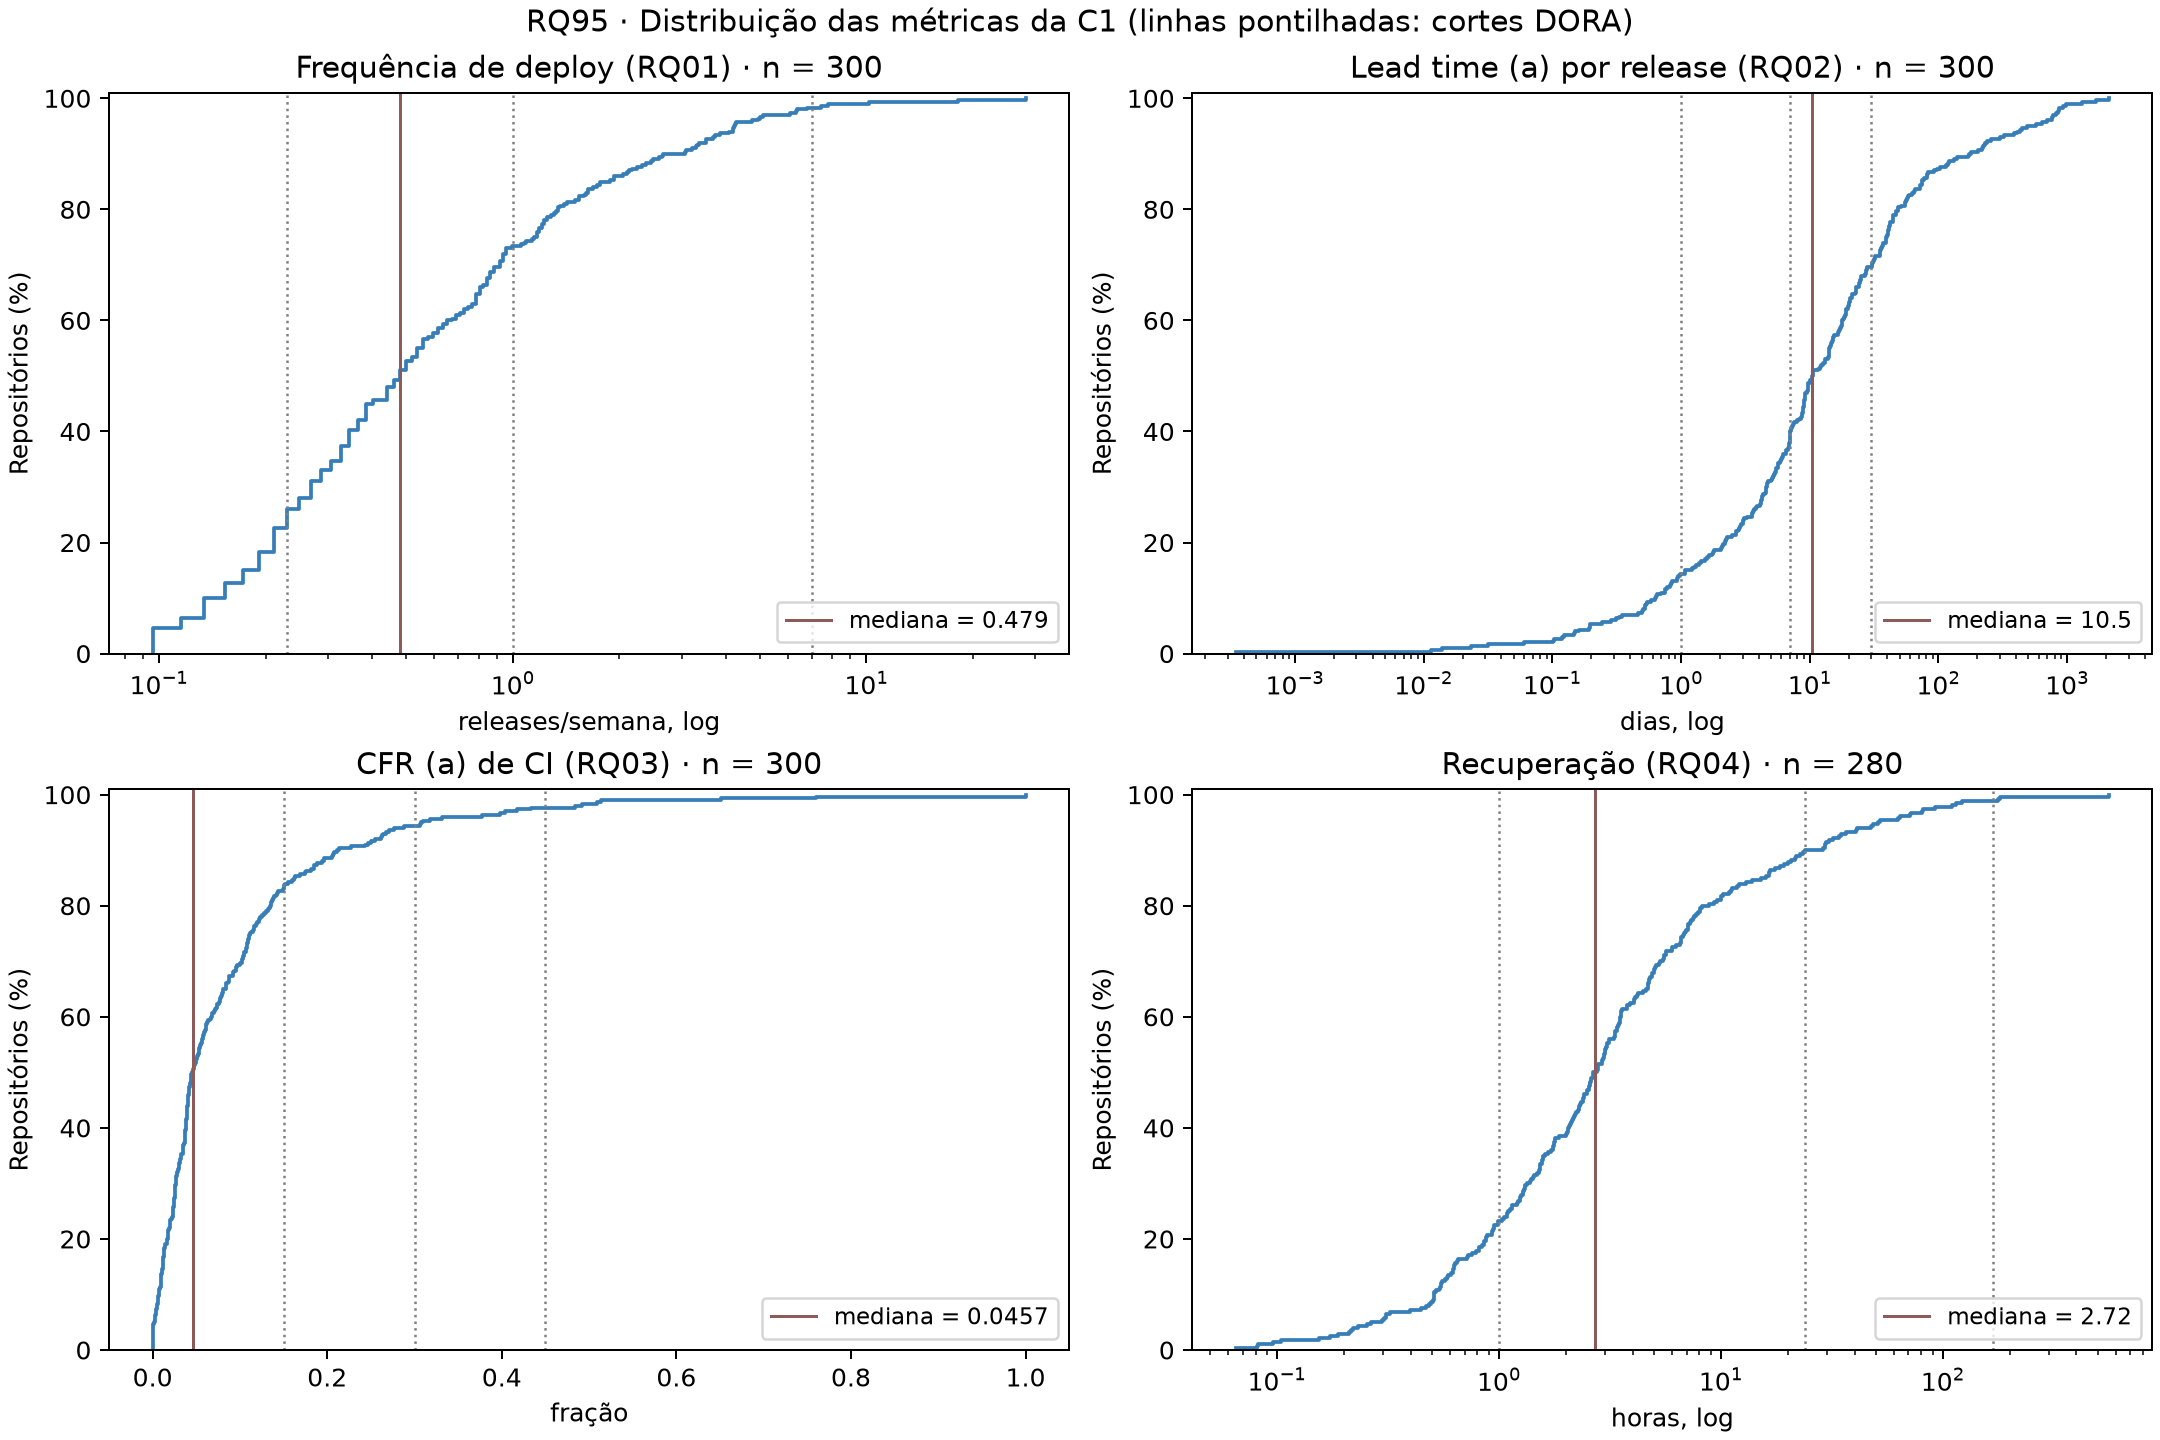
\includegraphics[width=0.92\linewidth]{figuras/distribuicoes_c1.png}
\caption{Distribuição acumulada das métricas da combinação C1 (linhas pontilhadas: cortes DORA;
linha vermelha: mediana).}
\label{fig:distribuicoes}
\end{figure}

\subsection{RQ01 --- Frequência de deploy}

A mediana é de 0,48 release/semana (IQR 0,93), com cauda longa à direita: o máximo é de 28,2
releases/semana e 33 repositórios passam do limite de Tukey (2,54). Os 30 repositórios mais
ativos (10\%) concentram 51,5\% das releases. Metade dos repositórios é Medium (50,7\%), um quarto é
High e só 5 (1,7\%) são Elite.

\subsection{RQ02 --- \textit{Lead time}}

Por release (a), a mediana é de 10,5 dias (IQR 35,9); por \textit{commit} (b), 12,1 dias (IQR 54,3).
Das 18.206 releases da janela, 14.589 têm \textit{lead time}; as demais são a primeira release
da história do repositório (57) ou não trazem \textit{commits} novos (3.560). A variante (b) é
menor que a (a) em 177 repositórios e maior em 122; a razão (b)/(a) tem mediana de 0,78 e o
teste de Wilcoxon pareado não rejeita a igualdade ($p = 0{,}12$). Trocar (a) por (b) muda a classe de
127 repositórios (42,3\%). Quanto maior a release, menor o (b) em relação ao (a)
($\rho = -0{,}30$ entre o número de \textit{commits} por release e a razão (b)/(a)).

\subsection{RQ03 --- Taxa de falha das mudanças}
\label{sec:rq03}

O CFR de CI (a) tem mediana de 4,6\% (IQR 8,8 pontos percentuais): 83,0\% dos repositórios são
Elite, e só 14 não têm nenhuma falha. O CFR de entrega (b), com a v1, tem mediana de 18,8\%
(IQR 44,7 pontos), muito mais disperso, e espalha os repositórios pelas quatro classes
(Tabela~\ref{tab:descritivo}). Somando todos os \textit{runs} e todas as releases, o CFR é de
9,2\% (a) e de 38,2\% (b). As duas variantes quase não concordam: $\rho = 0{,}07$ entre elas
($p = 0{,}26$), o (b) é maior que o (a) em 182 de 299 repositórios (Wilcoxon, $p < 10^{-15}$)
e 57,2\% dos repositórios mudam de classe ao trocar uma pela outra
($\kappa$ ponderado $= 0{,}02$, concordância leve), 144 deles para pior.

Os dois proxies medem coisas diferentes. No (a), 98,6\% das falhas são \texttt{failure} e 1,4\%
são \texttt{startup\_failure}, e o workflow que mais falha em cada repositório responde, na
mediana, por 73,1\% das falhas: o CFR (a) reflete sobretudo um ou dois \textit{workflows}. No
(b), 39,2\% das releases (7.130 de 18.206) têm tag fora do SemVer estrito e nunca são
corretivas na v1; 42 repositórios não têm nenhuma tag SemVer, e o CFR (b) deles é zero por
construção. Por outro lado, na mediana 42,9\% das releases de um repositório mudam só o
\textit{patch}. O nível do (b) depende da heurística: com as versões v2 (\textit{patch} ou qualquer
\textit{commit} com \texttt{fix}, \texttt{revert} ou \texttt{hotfix}) e v3 (correção de defeito),
a mediana vai a 43,5\% e 27,3\%, e 40,8\% e 31,8\% dos repositórios mudam de classe em relação à
v1. A v2 e a v3 marcam como corretivas 98,6\% e 61,3\% das releases na mediana, o que indica
excesso de marcações.

\begin{figure}[ht]
\centering
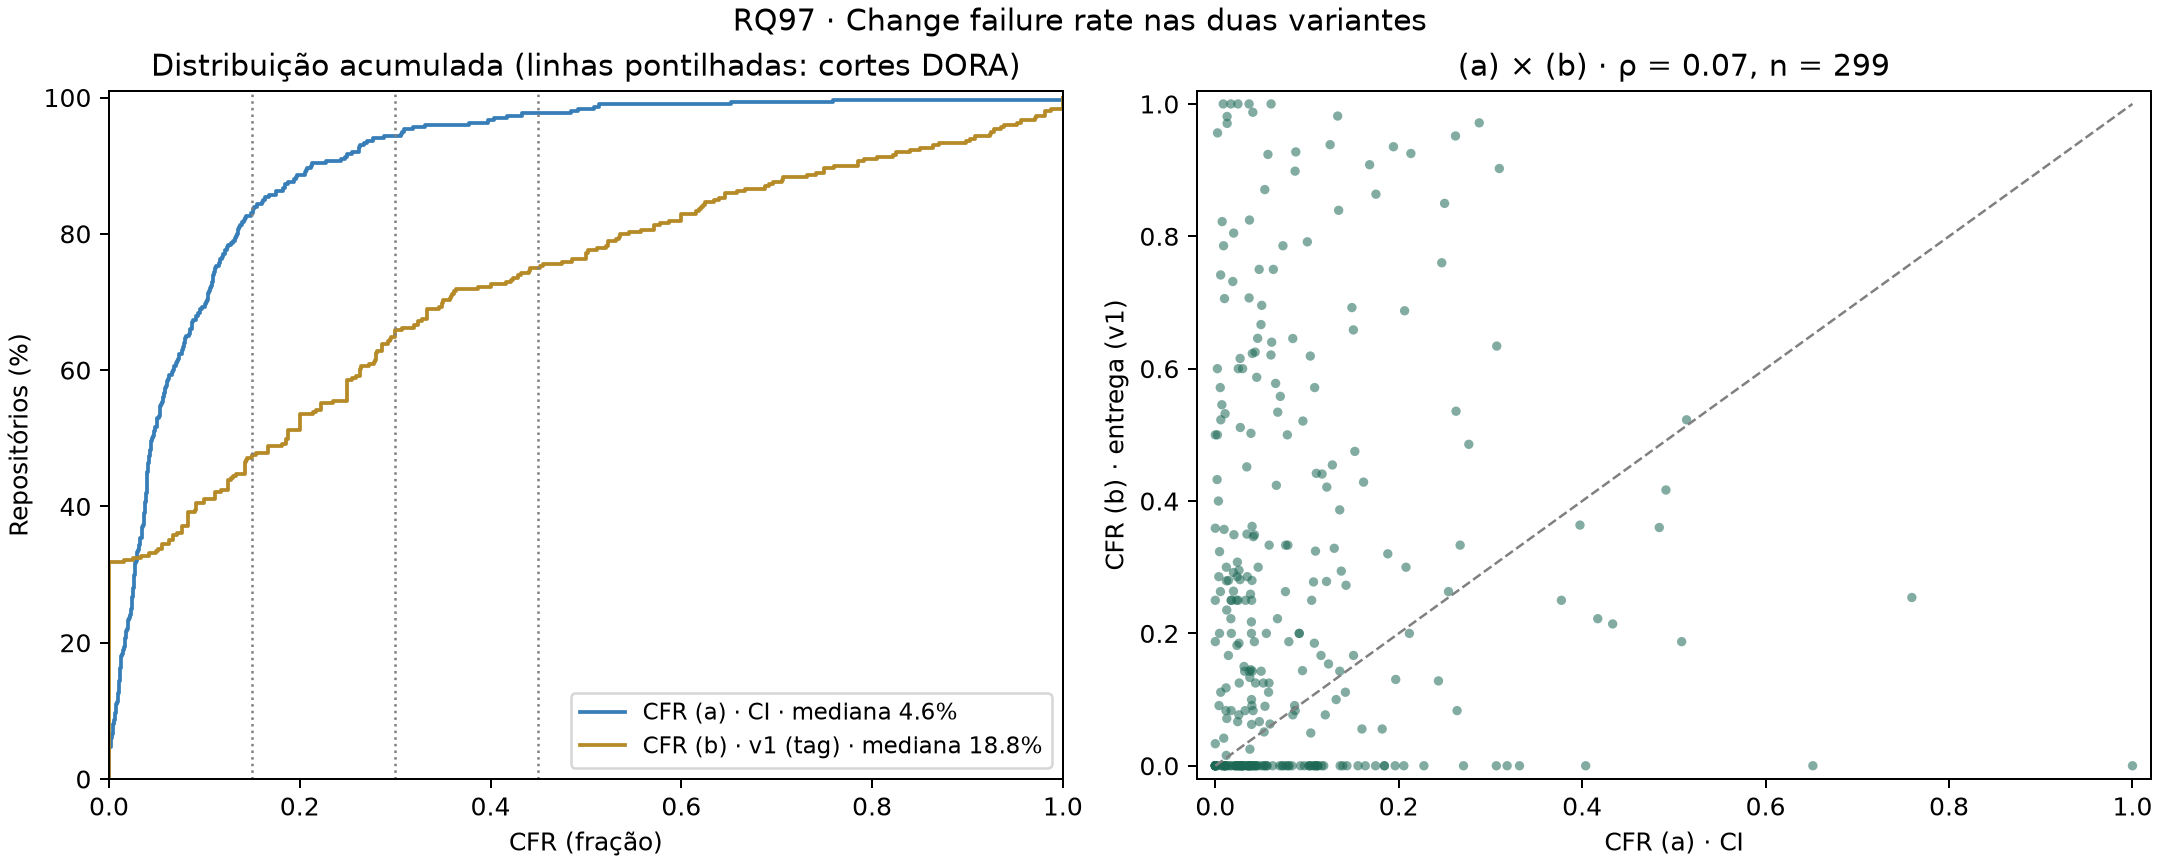
\includegraphics[width=0.95\linewidth]{figuras/cfr_variantes.png}
\caption{CFR nas duas variantes: distribuição acumulada (esquerda) e dispersão (a)~$\times$~(b)
(direita); linha tracejada: $y = x$.}
\label{fig:cfr}
\end{figure}

\subsection{RQ04 --- Tempo de recuperação}

Há 280 repositórios com tempo estimável (20 não têm nenhum episódio de falha completo e ficam
sem estimativa, não com zero). A mediana é de 2,7 horas (IQR 5,7), com cauda longa: o P90 é de
24,5 horas e o máximo, de 560 horas. Dos 27.839 episódios, 230 (0,83\%) terminam censurados à
direita, mas 24 repositórios têm pelo menos 10\% dos episódios censurados. Em 88,9\% dos
episódios a recuperação ocorre em até 24 horas (79,2\% com peso igual por repositório).

\subsection{Classificação DORA geral}

Pela combinação de referência C1 (release, \textit{lead time} (a), CFR (a)), 280 repositórios
recebem classe geral: 6,4\% Elite, 43,6\% High, 45,7\% Medium e 4,3\% Low; os 20 repositórios sem
episódio de falha completo ficam sem classe. A estabilidade é alta (Elite ou High nas duas métricas
da dimensão) em 85,4\% dos repositórios classificados, mas só 21,1\% têm velocidade alta. A classe
geral é limitada pela velocidade, não pela estabilidade.

\subsection{RQ05 --- Frequência de deploy e CFR}
\label{sec:rq05}

\begin{table}[ht]
\centering
\small
\caption{Correlação de Spearman entre a frequência de deploy e o CFR (IC de 95\% por
\textit{bootstrap}; $p$ com correção de Holm). O $\rho$ parcial controla idade e contribuidores
no (a) e o CFR (b) esperado ao acaso no (b) (Seção~\ref{sec:discussao}).}
\label{tab:rq05}
\begin{tabular}{lrrrrr}
\hline
Variante & $n$ & $\rho$ & $p$ (Holm) & IC 95\% & $\rho$ parcial \\
\hline
CFR (a), CI           & 300 & 0,15 & 0,009            & 0,04 a 0,27 & 0,09 ($p = 0{,}14$) \\
CFR (b), entrega (v1) & 299 & 0,40 & $2 \times 10^{-12}$ & 0,29 a 0,51 & $-0{,}16$ ($p = 0{,}005$) \\
\hline
\end{tabular}
\end{table}

A frequência de deploy tem correlação fraca e positiva com o CFR (a) e moderada e positiva com o CFR (b)
(Tabela~\ref{tab:rq05}, Figura~\ref{fig:rq05}). Em quartis de frequência, a mediana do CFR (a) fica
em torno de 4--7\% em todas as faixas, enquanto a do CFR (b) sobe de 0\% (Q1) para 44,2\% (Q4).
Em termos de classes, 94\% dos repositórios de frequência alta (Elite ou High) têm CFR (a) Elite
ou High, contra 95\% dos de frequência baixa (Fisher, $p = 0{,}78$); no CFR (b), 40\% contra 75\%
($p < 10^{-7}$).

\begin{figure}[ht]
\centering
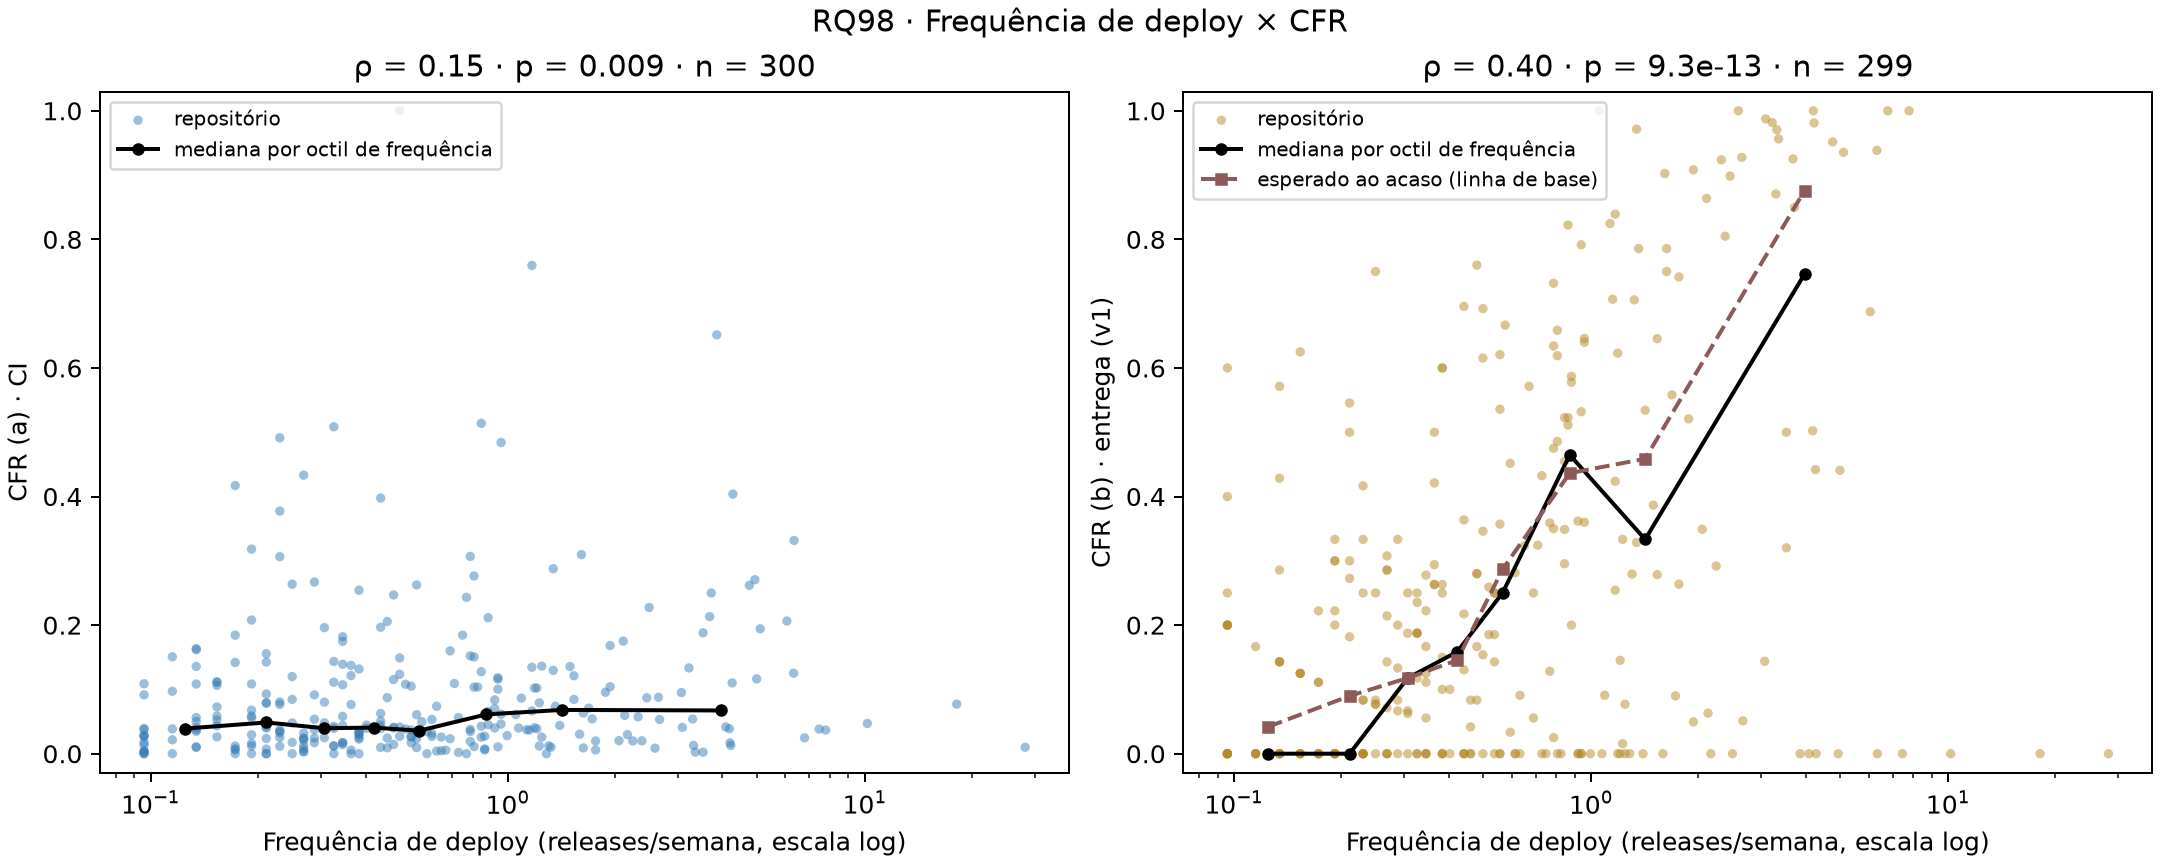
\includegraphics[width=0.95\linewidth]{figuras/dispersao_df_cfr.png}
\caption{Frequência de deploy (escala logarítmica) e CFR. Linha preta: mediana por octil de
frequência; linha tracejada: CFR (b) esperado ao acaso (linha de base da Seção~\ref{sec:discussao}).}
\label{fig:rq05}
\end{figure}

\subsection{RQ06 --- Características dos repositórios}
\label{sec:rq06}

\apreencher{resultados da RQ06 (issue \#93): Kruskal-Wallis ou Mann-Whitney por fator, p-valores
com correção de Holm, $\varepsilon^2$ e $\delta$ de Cliff}

\subsection{RQ07 --- Sensibilidade da classificação DORA}

Classificamos cada repositório em sete combinações de definições (C1 a C7, Tabela~\ref{tab:rq07}).
Dos 279 repositórios classificados em todas elas, 163 (58,4\%) têm a mesma classe geral em todas
e 116 (41,6\%) mudam em pelo menos uma alternativa à C1. Trocar só a unidade de deploy (C5 e C6)
muda de 3,6\% a 10,7\% das classes, sempre para melhor ($\kappa$ de 0,85 a 0,95); as
combinações com o CFR (b) mudam de 20,8\% a 35,5\%, e 75\% das mudanças são para pior. No nível
de cada métrica, trocar o CFR (a) pelo (b) muda a classe de 57,2\% dos repositórios
($\kappa = 0{,}02$), o \textit{lead time} (a) pelo (b), de 42,3\%, e a unidade de deploy de
release para tag, de 24,0\%.

\begin{table}[ht]
\centering
\small
\caption{Mudança da classe geral em relação à C1 (279 a 280 repositórios por par).}
\label{tab:rq07}
\begin{tabular}{llrrl}
\hline
Combinação & O que muda em relação à C1 & Mudam (\%) & $\kappa$ pond. & Landis--Koch \\
\hline
C2 & \textit{lead time} (b)                     & 14,3 & 0,79 & substancial \\
C3 & CFR (b)                                    & 20,8 & 0,68 & substancial \\
C4 & \textit{lead time} (b) e CFR (b)           & 29,7 & 0,52 & moderada \\
C5 & pré-releases contam como deploy            & 3,6  & 0,95 & quase perfeita \\
C6 & tags contam como deploy                    & 10,7 & 0,85 & quase perfeita \\
C7 & tags, \textit{lead time} (b) e CFR (b)     & 35,5 & 0,44 & moderada \\
\hline
\end{tabular}
\end{table}
.
% Os numeros vem das mesmas analises da Secao 3 (entregas/laboratorio-03/sprint-03, RQ91 a RQ98).
% Trechos em \apreencher{...} dependem da RQ06 (issue #93) e da validacao manual (issues #85 a #89).

\providecommand{\apreencher}[1]{\textbf{[a preencher: #1]}}

\section{Discussão}
\label{sec:discussao}

\subsection{Hipóteses e resultados}

A Tabela~\ref{tab:hipoteses} confronta cada hipótese informal da Seção~\ref{sec:hipoteses},
registrada antes da análise, com o que encontramos. Nenhuma faixa prevista foi alterada depois
da análise.

\begin{table}[ht]
\centering
\scriptsize
\caption{Hipóteses (Seção~\ref{sec:hipoteses}) frente aos resultados (Seção~\ref{sec:resultados}).}
\label{tab:hipoteses}
\begin{tabular}{p{0.05\linewidth}p{0.28\linewidth}p{0.40\linewidth}p{0.15\linewidth}}
\hline
 & Previsão & Resultado & Veredito \\
\hline
H1 & Mediana de 0,5 a 1 release/semana; Medium e High; cauda longa; poucos Elite
   & Mediana de 0,48; Medium e High somam 75,7\%; 33 extremos; 1,7\% Elite
   & Confirmada, com a mediana pouco abaixo da faixa \\
H2 & (a) em semanas (Medium ou Low); (b) sistematicamente menor; diferença cresce com o tamanho da release
   & (a) = 10,5 dias, com 60,7\% em Medium ou Low; (b) = 12,1 dias, menor em 177 de 300 repositórios, mas
     sem diferença pareada ($p = 0{,}12$); $\rho = -0{,}30$ com o tamanho
   & Parcial: (a) e o efeito do tamanho sim; (b) menor, não \\
H3 & CFR (a) de 10 a 25\%; (b) de 5 a 15\% e mais variável; $|\rho| < 0{,}3$ entre (a) e (b)
   & (a) = 4,6\%; (b) = 18,8\%, com IQR de 44,7 contra 8,8 pontos; $\rho = 0{,}07$
   & Parcial (2 de 4): variabilidade e correlação sim; níveis, não \\
H4 & Recuperação de 1 hora a 1 dia; cauda longa; censura abaixo de 10\%
   & 2,7 horas; P90 de 24,5 horas e máximo de 560; censura de 0,83\% (24 repositórios com $\geq 10$\%)
   & Confirmada \\
H5 & $\rho$ próximo de zero ou levemente negativo no (b) e próximo de zero no (a)
   & (a) $\rho = 0{,}15$; (b) $\rho = 0{,}40$, ou $-0{,}16$ após a linha de base
   & Parcial: vale, fracamente, no (a); não vale no (b) bruto \\
H6 & Efeitos pequenos a médios; contribuidores, tipo e linguagem associados
   & \apreencher{RQ06 (issue \#93)}
   & Pendente \\
H7 & $\geq 30$\% mudam de classe; $\kappa$ de 0,2 a 0,6; pré-releases e tags inflam a frequência; \textit{lead time} (b) melhora a classe
   & 1 de 6 alternativas com $\geq 30$\% (C7: 35,5\%); $\kappa$ de 0,44 a 0,95; pré-releases e tags só melhoram a classe de frequência; (b) melhora 61 repositórios e piora 66
   & Parcial: depende de qual definição muda \\
\hline
\end{tabular}
\end{table}

\subsection{O que surpreendeu e por quê}

\textbf{A velocidade é o gargalo; a estabilidade quase nunca.} Esperávamos CFR de CI entre 10\% e
25\% e encontramos 4,6\%. Com o corte de Elite em 15\%, 83\% dos repositórios são Elite no CFR (a),
e 85,4\% têm estabilidade alta contra 21,1\% com velocidade alta. O resultado é coerente com o
perfil da amostra, projetos populares com CI madura, mas também com a natureza do proxy: o CFR (a)
mede falha de pipeline, concentrada em um ou dois \textit{workflows} (73,1\% das falhas, na mediana),
e não mede defeito que chega ao usuário. Os cortes DORA vêm de questionários com empresas; aqui o
CFR (a) discrimina pouco, e a classe geral fica presa à frequência e ao \textit{lead time}. Já a
frequência baixa tem uma leitura própria: uma biblioteca que publica uma release por mês não está
``deployando'' nada, e a classe Medium da maioria dos repositórios reflete o ritmo de publicação,
não necessariamente uma entrega lenta.

\textbf{Os dois CFR respondem a perguntas diferentes.} O CFR (b) não ficou abaixo do (a), como
previsto, e a correlação entre eles é desprezível ($\rho = 0{,}07$); 57,2\% dos repositórios mudam de
classe ao trocar um pelo outro. A previsão de que medem fenômenos distintos se confirmou, mas o
nível do (b) é frágil: depende de uma heurística cuja versão v1 deixa de fora 39,2\% das releases
(tags fora do SemVer), e a mediana vai de 18,8\% a 43,5\% conforme a versão
(Seção~\ref{sec:rq03}). Sem o F1 contra o consenso da amostra-ouro (\apreencher{P, R e F1 das versões
da heurística e $\kappa$ de Fleiss entre os avaliadores}), não sabemos qual dessas taxas se aproxima da
taxa real de releases corretivas; por isso reportamos as duas variantes e não escolhemos a mais
favorável a uma hipótese.

\textbf{Mais releases, mais CFR (b), mas por aritmética.} Esperávamos ausência de \textit{trade-off}, em
linha com o DORA. O $\rho$ bruto entre frequência e CFR (b) foi de $0{,}40$, e 40\% dos repositórios de
frequência alta têm CFR (b) Elite ou High, contra 75\% dos de frequência baixa. Lido sem cuidado, isso
sugeriria que publicar mais piora a estabilidade. Mas o CFR (b) conta uma falha quando alguma release
\textit{patch} sai em até 7 dias, e quanto mais releases, maior a chance de isso acontecer ao acaso: a fração
de releases com alguma sucessora em 7 dias tem $\rho = 0{,}83$ com a frequência, enquanto a proporção de
\textit{patches} quase não varia com ela. Embaralhando, em cada repositório, quais releases são corretivas,
o CFR (b) esperado ao acaso tem $\rho = 0{,}59$ com a frequência, acima do observado, e o $\rho$ parcial,
controlando esse esperado, é $-0{,}16$. Para o CFR (a), a relação é fraca ($\rho = 0{,}15$) e perde a
significância ao controlar idade e contribuidores ($0{,}09$; $p = 0{,}14$). Assim, os dados
\textit{open source} não confirmam nem contradizem a afirmação do DORA de que velocidade e estabilidade
andam juntas: o proxy de entrega tem um acoplamento aritmético com a frequência, e o de CI quase não
discrimina. Correlação não implica causalidade; tamanho da equipe, maturidade e automação de
releases podem afetar as duas medidas.

\textbf{\textit{Lead time} por \textit{commit} não é menor que por release.} Previmos o (b) sistematicamente
menor, porque um \textit{commit} antigo ``esquecido'' infla o (a) e é diluído no (b). O mecanismo aparece nas
releases grandes ($\rho = -0{,}30$ entre o tamanho e a razão (b)/(a)), mas o (b) pondera as releases pelo
número de \textit{commits}: onde poucas releases grandes concentram \textit{commits} antigos e muitas releases
pequenas são rápidas, a mediana por \textit{commit} cai dentro das grandes e supera a por release. No
agregado, as variantes divergem em ambos os sentidos, e o teste pareado não as separa.

\textbf{A classificação é frágil, mas não a todas as escolhas.} Dos repositórios classificados em todas as
combinações, 41,6\% mudam de classe em pelo menos uma alternativa, e o efeito não é uniforme: trocar a
unidade de deploy muda de 3,6\% a 10,7\% das classes, sempre para melhor ($\kappa \geq 0{,}85$), enquanto as
combinações com o CFR (b) mudam de 20,8\% a 35,5\%, em geral para pior ($\kappa$ de 0,44 a 0,68). Como o CFR (b) depende de uma heurística
ainda sem F1, parte desse efeito pode ser do proxy, não da definição. As conclusões das RQ01 a RQ05
valem, portanto, para a combinação C1 e são condicionais à definição de falha, e menos à de deploy.

\subsection{Implicações}

Para quem minera métricas DORA no GitHub, três cuidados decorrem dos resultados. Primeiro, release
não é deploy, e falha de CI não é falha em produção; as classes servem para comparar repositórios entre si,
não para dizer que um projeto de código aberto é ``Elite'' no sentido do DORA. Segundo, o CFR
baseado em releases corretivas só tem sentido com uma heurística validada contra julgamento humano, e
deve ser comparado ao que o acaso produziria quando a frequência de releases é alta. Terceiro, vale
reportar a sensibilidade às definições, como fizemos na RQ07, porque a escolha do CFR por si só
reclassifica de 20,8\% a 35,5\% dos repositórios. A RQ06 (características dos repositórios)
ainda não foi analisada (\apreencher{discussão da RQ06 e da H6}); as ameaças à validade que decorrem
destes achados estão na Seção~5.
 depois de % Secao 3 do artigo do LAB03 (template SBC). Issue #99.
% Uso no Overleaf: % Secao 3 do artigo do LAB03 (template SBC). Issue #99.
% Uso no Overleaf: \input{resultados} depois de \input{metodologia}; as figuras ficam em figuras/
% (\usepackage{graphicx}, ja no template).
%
% Todos os numeros vem das analises do repositorio (entregas/laboratorio-03/sprint-03):
% RQ91 (RQ01), RQ94 (RQ02), RQ97 (RQ03), RQ92 (RQ04), RQ95 (classificacao C1),
% RQ98 (RQ05), RQ96 (RQ07). Janela provisoria; CFR (b) com a heuristica v1, ainda sem F1 medido.
% Trechos em \apreencher{...} dependem de analises ainda nao feitas (RQ06, issue #93) ou da
% validacao manual (issues #85 a #89). Busque por "apreencher" antes de entregar.

\providecommand{\apreencher}[1]{\textbf{[a preencher: #1]}}

\section{Resultados}
\label{sec:resultados}

Os resultados se referem aos 300 repositórios da amostra final (Seção~\ref{sec:funil}),
na janela de 01/10/2025 a 30/09/2026, ainda provisória (Seção~\ref{sec:definicoes}). Cada
repositório tem o mesmo peso e a estatística da amostra é a mediana dos valores dos
repositórios, com o intervalo interquartil (IQR, Q1--Q3). A Tabela~\ref{tab:descritivo} resume
as métricas e a classificação DORA de cada uma. Nas Seções~\ref{sec:rq03} e~\ref{sec:rq05},
o CFR (b) usa a versão v1 da heurística de release corretiva, que ainda não tem F1 medido
contra o consenso da amostra-ouro (\apreencher{P, R e F1 das versões v1, v2 e v3}).

\begin{table}[ht]
\centering
\small
\caption{Métricas DORA e classes (\% dos repositórios com a métrica definida). Frequência em
releases/semana; \textit{lead time} em dias; CFR em \%; recuperação em horas.}
\label{tab:descritivo}
\begin{tabular}{lrrrrrr}
\hline
Métrica & $n$ & Mediana (Q1--Q3) & Elite & High & Medium & Low \\
\hline
Frequência de deploy      & 300 & 0,48 (0,23--1,16) & 1,7  & 25,0 & 50,7 & 22,7 \\
\textit{Lead time} (a)    & 300 & 10,5 (3,6--39,5)  & 14,3 & 25,0 & 30,3 & 30,3 \\
\textit{Lead time} (b)    & 300 & 12,1 (3,3--57,5)  & 10,3 & 28,7 & 28,7 & 32,3 \\
CFR (a), CI               & 300 & 4,6 (2,3--11,1)   & 83,0 & 11,3 & 3,3  & 2,3  \\
CFR (b), entrega (v1)     & 299 & 18,8 (0,0--44,7)  & 47,5 & 18,4 & 9,0  & 25,1 \\
Recuperação               & 280 & 2,7 (1,1--6,9)    & 23,2 & 66,4 & 9,3  & 1,1  \\
\hline
Classe geral (C1)         & 280 & ---               & 6,4  & 43,6 & 45,7 & 4,3  \\
\hline
\end{tabular}
\end{table}

\begin{figure}[ht]
\centering
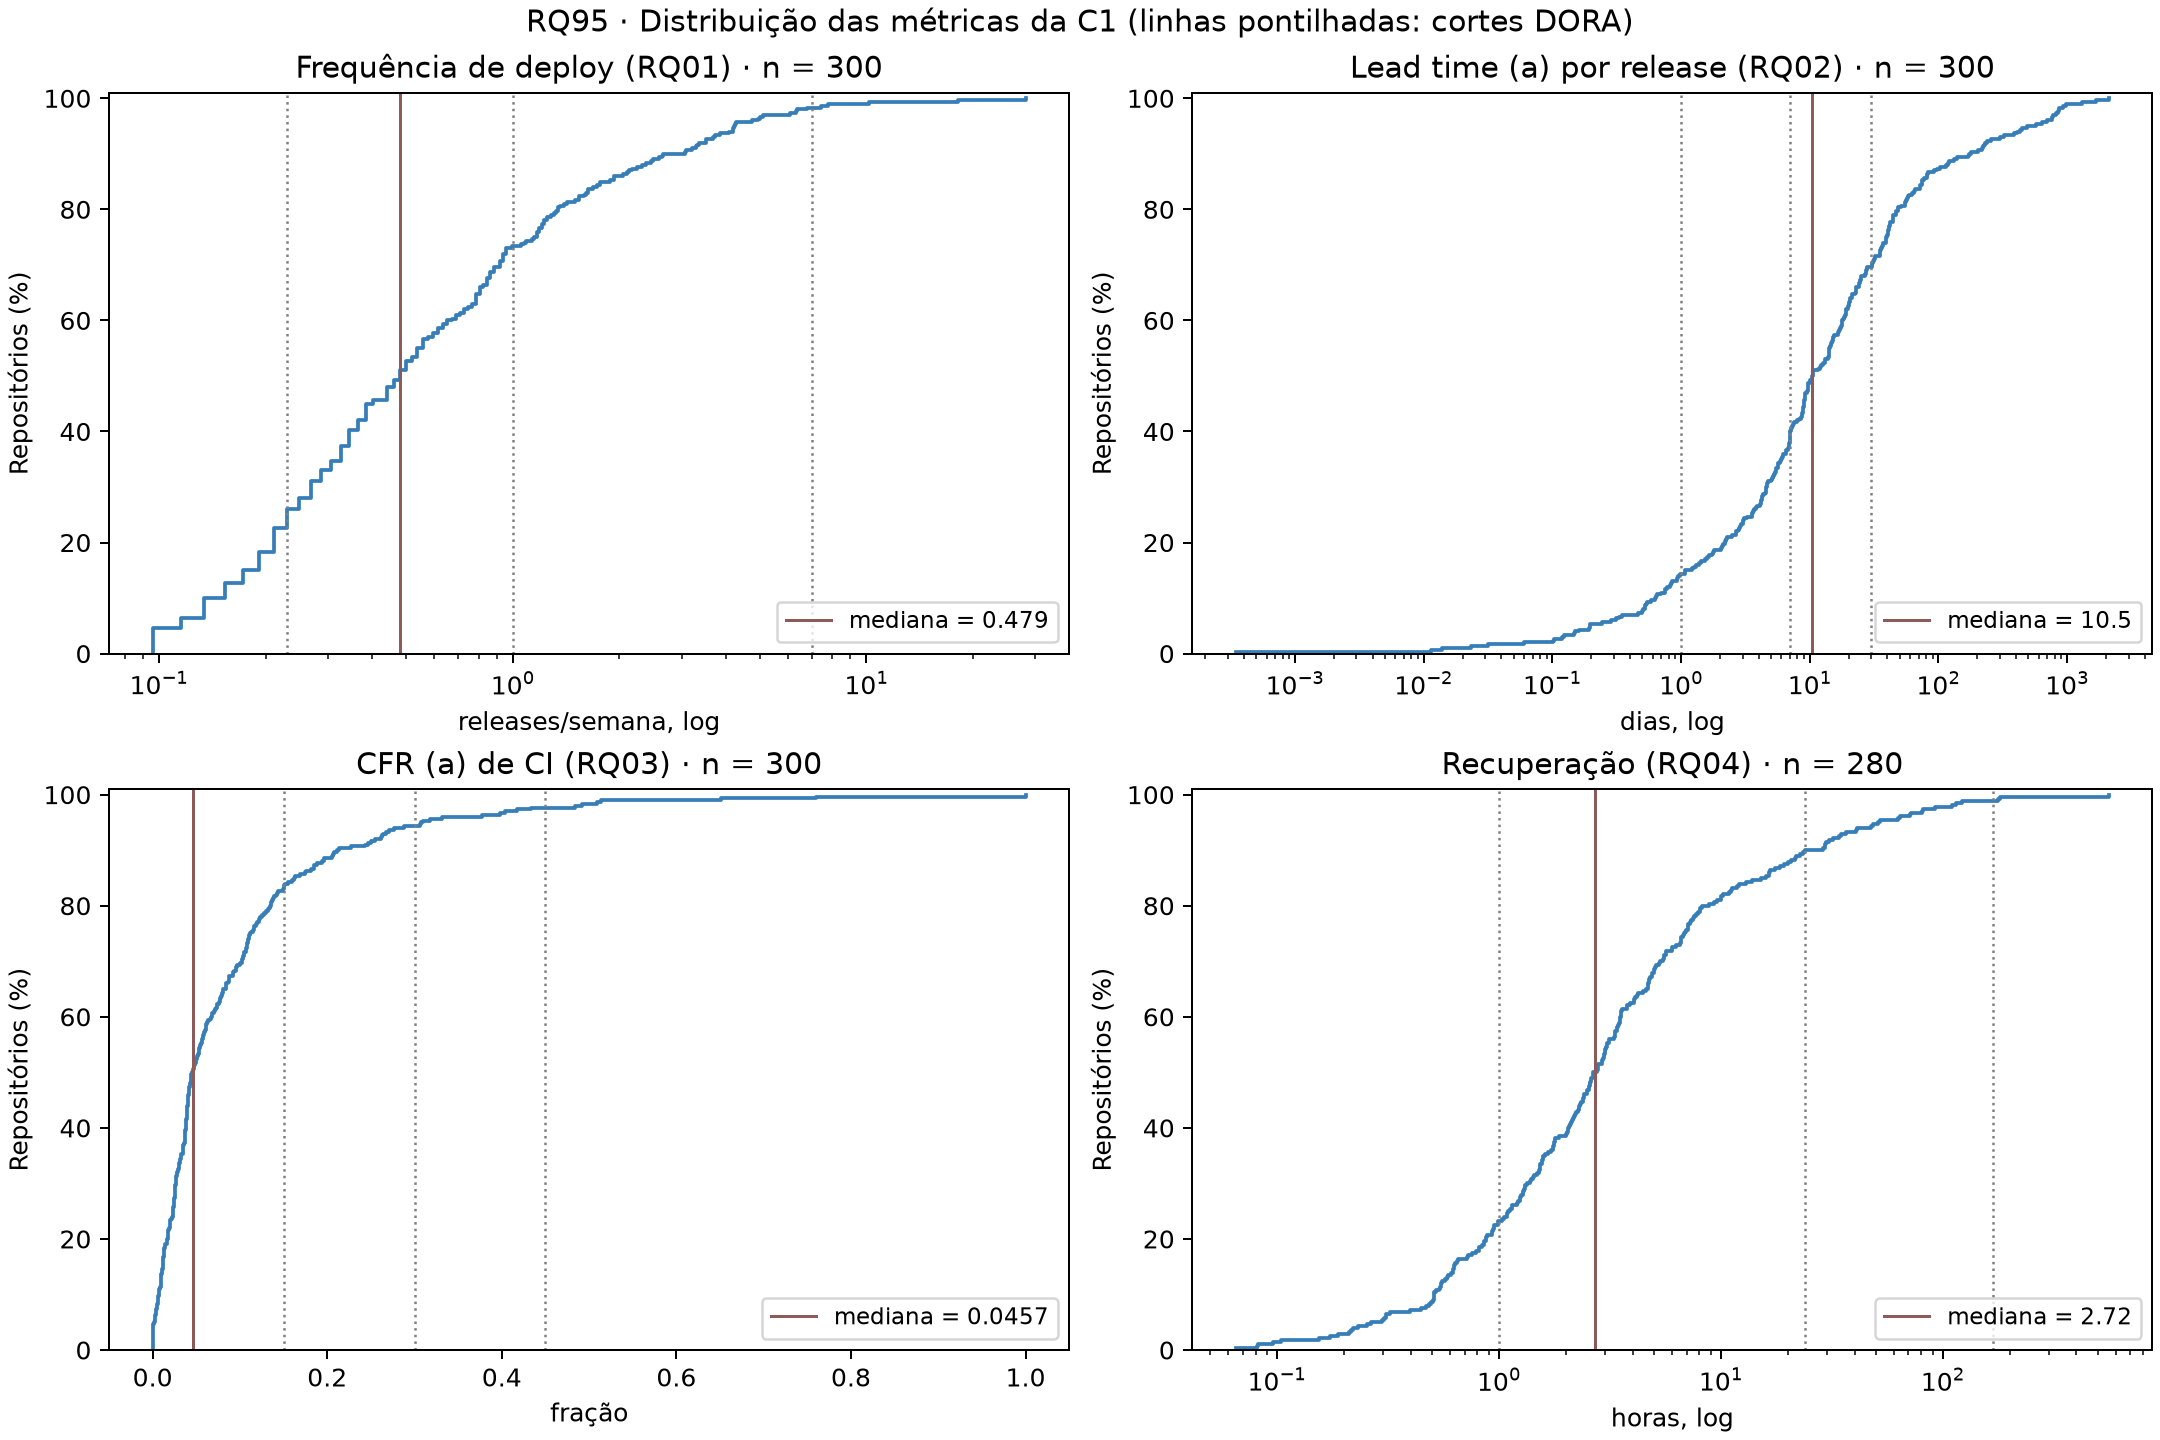
\includegraphics[width=0.92\linewidth]{figuras/distribuicoes_c1.png}
\caption{Distribuição acumulada das métricas da combinação C1 (linhas pontilhadas: cortes DORA;
linha vermelha: mediana).}
\label{fig:distribuicoes}
\end{figure}

\subsection{RQ01 --- Frequência de deploy}

A mediana é de 0,48 release/semana (IQR 0,93), com cauda longa à direita: o máximo é de 28,2
releases/semana e 33 repositórios passam do limite de Tukey (2,54). Os 30 repositórios mais
ativos (10\%) concentram 51,5\% das releases. Metade dos repositórios é Medium (50,7\%), um quarto é
High e só 5 (1,7\%) são Elite.

\subsection{RQ02 --- \textit{Lead time}}

Por release (a), a mediana é de 10,5 dias (IQR 35,9); por \textit{commit} (b), 12,1 dias (IQR 54,3).
Das 18.206 releases da janela, 14.589 têm \textit{lead time}; as demais são a primeira release
da história do repositório (57) ou não trazem \textit{commits} novos (3.560). A variante (b) é
menor que a (a) em 177 repositórios e maior em 122; a razão (b)/(a) tem mediana de 0,78 e o
teste de Wilcoxon pareado não rejeita a igualdade ($p = 0{,}12$). Trocar (a) por (b) muda a classe de
127 repositórios (42,3\%). Quanto maior a release, menor o (b) em relação ao (a)
($\rho = -0{,}30$ entre o número de \textit{commits} por release e a razão (b)/(a)).

\subsection{RQ03 --- Taxa de falha das mudanças}
\label{sec:rq03}

O CFR de CI (a) tem mediana de 4,6\% (IQR 8,8 pontos percentuais): 83,0\% dos repositórios são
Elite, e só 14 não têm nenhuma falha. O CFR de entrega (b), com a v1, tem mediana de 18,8\%
(IQR 44,7 pontos), muito mais disperso, e espalha os repositórios pelas quatro classes
(Tabela~\ref{tab:descritivo}). Somando todos os \textit{runs} e todas as releases, o CFR é de
9,2\% (a) e de 38,2\% (b). As duas variantes quase não concordam: $\rho = 0{,}07$ entre elas
($p = 0{,}26$), o (b) é maior que o (a) em 182 de 299 repositórios (Wilcoxon, $p < 10^{-15}$)
e 57,2\% dos repositórios mudam de classe ao trocar uma pela outra
($\kappa$ ponderado $= 0{,}02$, concordância leve), 144 deles para pior.

Os dois proxies medem coisas diferentes. No (a), 98,6\% das falhas são \texttt{failure} e 1,4\%
são \texttt{startup\_failure}, e o workflow que mais falha em cada repositório responde, na
mediana, por 73,1\% das falhas: o CFR (a) reflete sobretudo um ou dois \textit{workflows}. No
(b), 39,2\% das releases (7.130 de 18.206) têm tag fora do SemVer estrito e nunca são
corretivas na v1; 42 repositórios não têm nenhuma tag SemVer, e o CFR (b) deles é zero por
construção. Por outro lado, na mediana 42,9\% das releases de um repositório mudam só o
\textit{patch}. O nível do (b) depende da heurística: com as versões v2 (\textit{patch} ou qualquer
\textit{commit} com \texttt{fix}, \texttt{revert} ou \texttt{hotfix}) e v3 (correção de defeito),
a mediana vai a 43,5\% e 27,3\%, e 40,8\% e 31,8\% dos repositórios mudam de classe em relação à
v1. A v2 e a v3 marcam como corretivas 98,6\% e 61,3\% das releases na mediana, o que indica
excesso de marcações.

\begin{figure}[ht]
\centering
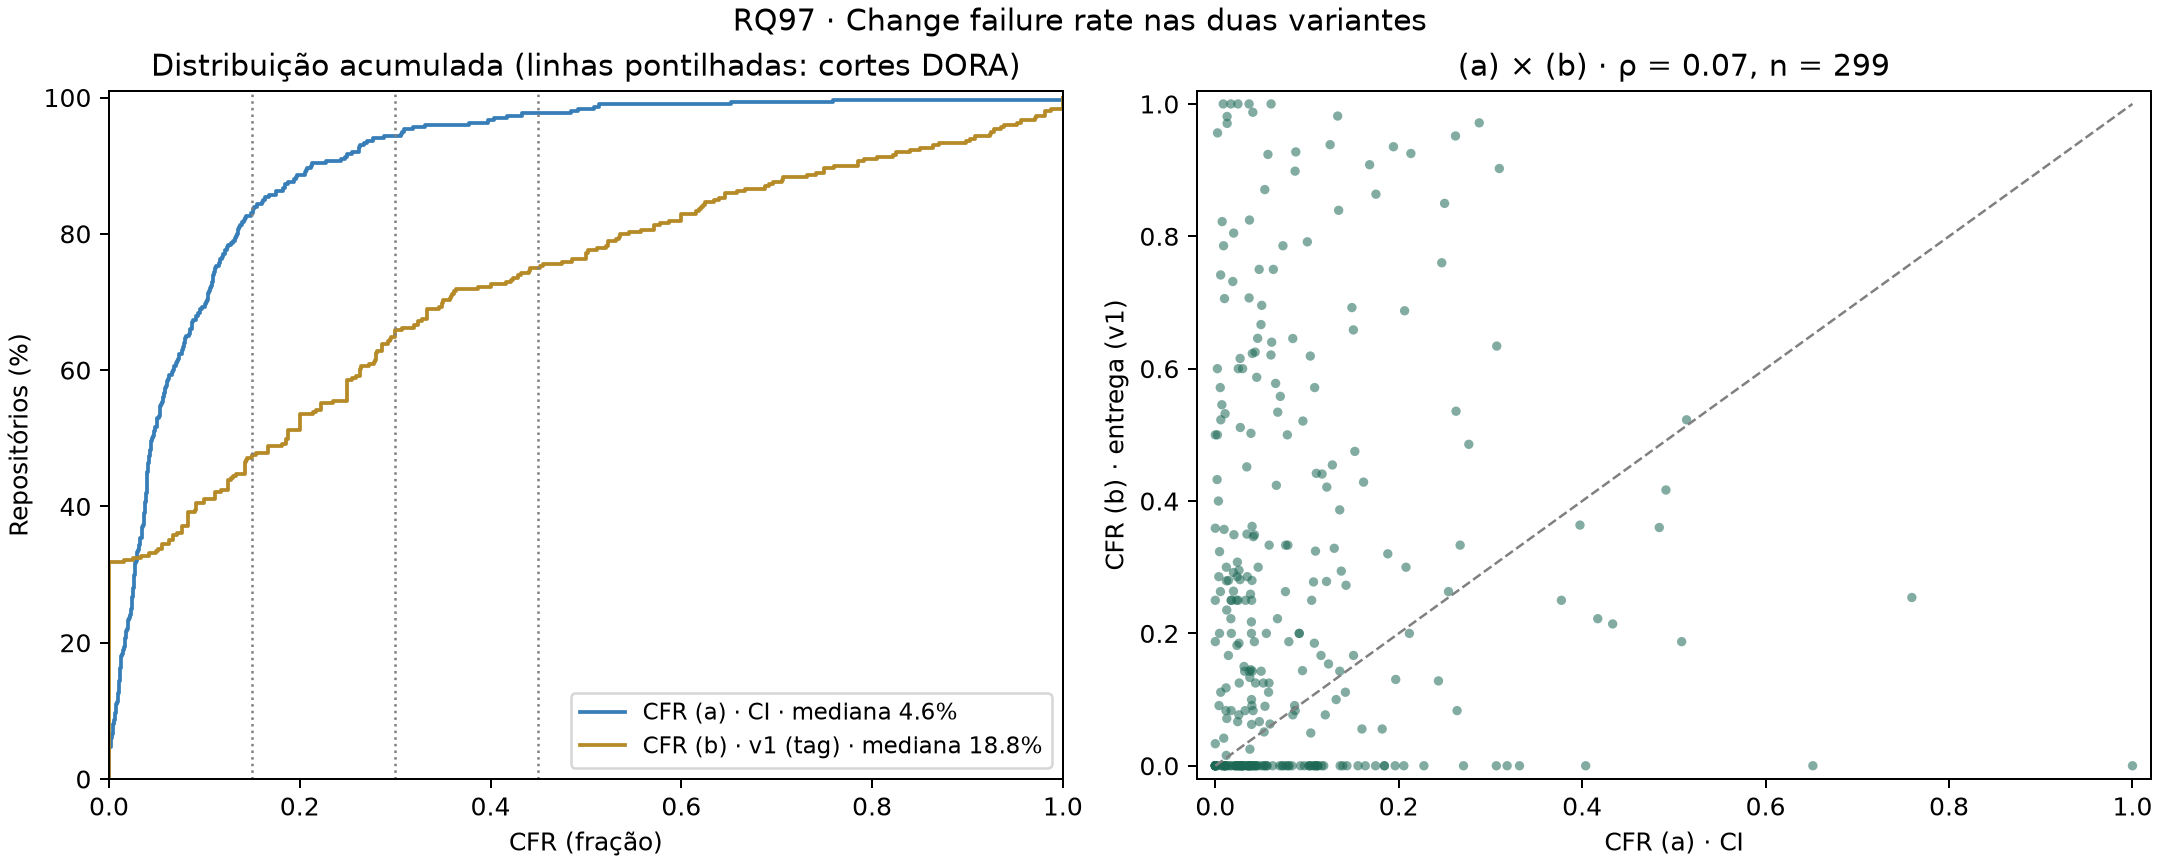
\includegraphics[width=0.95\linewidth]{figuras/cfr_variantes.png}
\caption{CFR nas duas variantes: distribuição acumulada (esquerda) e dispersão (a)~$\times$~(b)
(direita); linha tracejada: $y = x$.}
\label{fig:cfr}
\end{figure}

\subsection{RQ04 --- Tempo de recuperação}

Há 280 repositórios com tempo estimável (20 não têm nenhum episódio de falha completo e ficam
sem estimativa, não com zero). A mediana é de 2,7 horas (IQR 5,7), com cauda longa: o P90 é de
24,5 horas e o máximo, de 560 horas. Dos 27.839 episódios, 230 (0,83\%) terminam censurados à
direita, mas 24 repositórios têm pelo menos 10\% dos episódios censurados. Em 88,9\% dos
episódios a recuperação ocorre em até 24 horas (79,2\% com peso igual por repositório).

\subsection{Classificação DORA geral}

Pela combinação de referência C1 (release, \textit{lead time} (a), CFR (a)), 280 repositórios
recebem classe geral: 6,4\% Elite, 43,6\% High, 45,7\% Medium e 4,3\% Low; os 20 repositórios sem
episódio de falha completo ficam sem classe. A estabilidade é alta (Elite ou High nas duas métricas
da dimensão) em 85,4\% dos repositórios classificados, mas só 21,1\% têm velocidade alta. A classe
geral é limitada pela velocidade, não pela estabilidade.

\subsection{RQ05 --- Frequência de deploy e CFR}
\label{sec:rq05}

\begin{table}[ht]
\centering
\small
\caption{Correlação de Spearman entre a frequência de deploy e o CFR (IC de 95\% por
\textit{bootstrap}; $p$ com correção de Holm). O $\rho$ parcial controla idade e contribuidores
no (a) e o CFR (b) esperado ao acaso no (b) (Seção~\ref{sec:discussao}).}
\label{tab:rq05}
\begin{tabular}{lrrrrr}
\hline
Variante & $n$ & $\rho$ & $p$ (Holm) & IC 95\% & $\rho$ parcial \\
\hline
CFR (a), CI           & 300 & 0,15 & 0,009            & 0,04 a 0,27 & 0,09 ($p = 0{,}14$) \\
CFR (b), entrega (v1) & 299 & 0,40 & $2 \times 10^{-12}$ & 0,29 a 0,51 & $-0{,}16$ ($p = 0{,}005$) \\
\hline
\end{tabular}
\end{table}

A frequência de deploy tem correlação fraca e positiva com o CFR (a) e moderada e positiva com o CFR (b)
(Tabela~\ref{tab:rq05}, Figura~\ref{fig:rq05}). Em quartis de frequência, a mediana do CFR (a) fica
em torno de 4--7\% em todas as faixas, enquanto a do CFR (b) sobe de 0\% (Q1) para 44,2\% (Q4).
Em termos de classes, 94\% dos repositórios de frequência alta (Elite ou High) têm CFR (a) Elite
ou High, contra 95\% dos de frequência baixa (Fisher, $p = 0{,}78$); no CFR (b), 40\% contra 75\%
($p < 10^{-7}$).

\begin{figure}[ht]
\centering
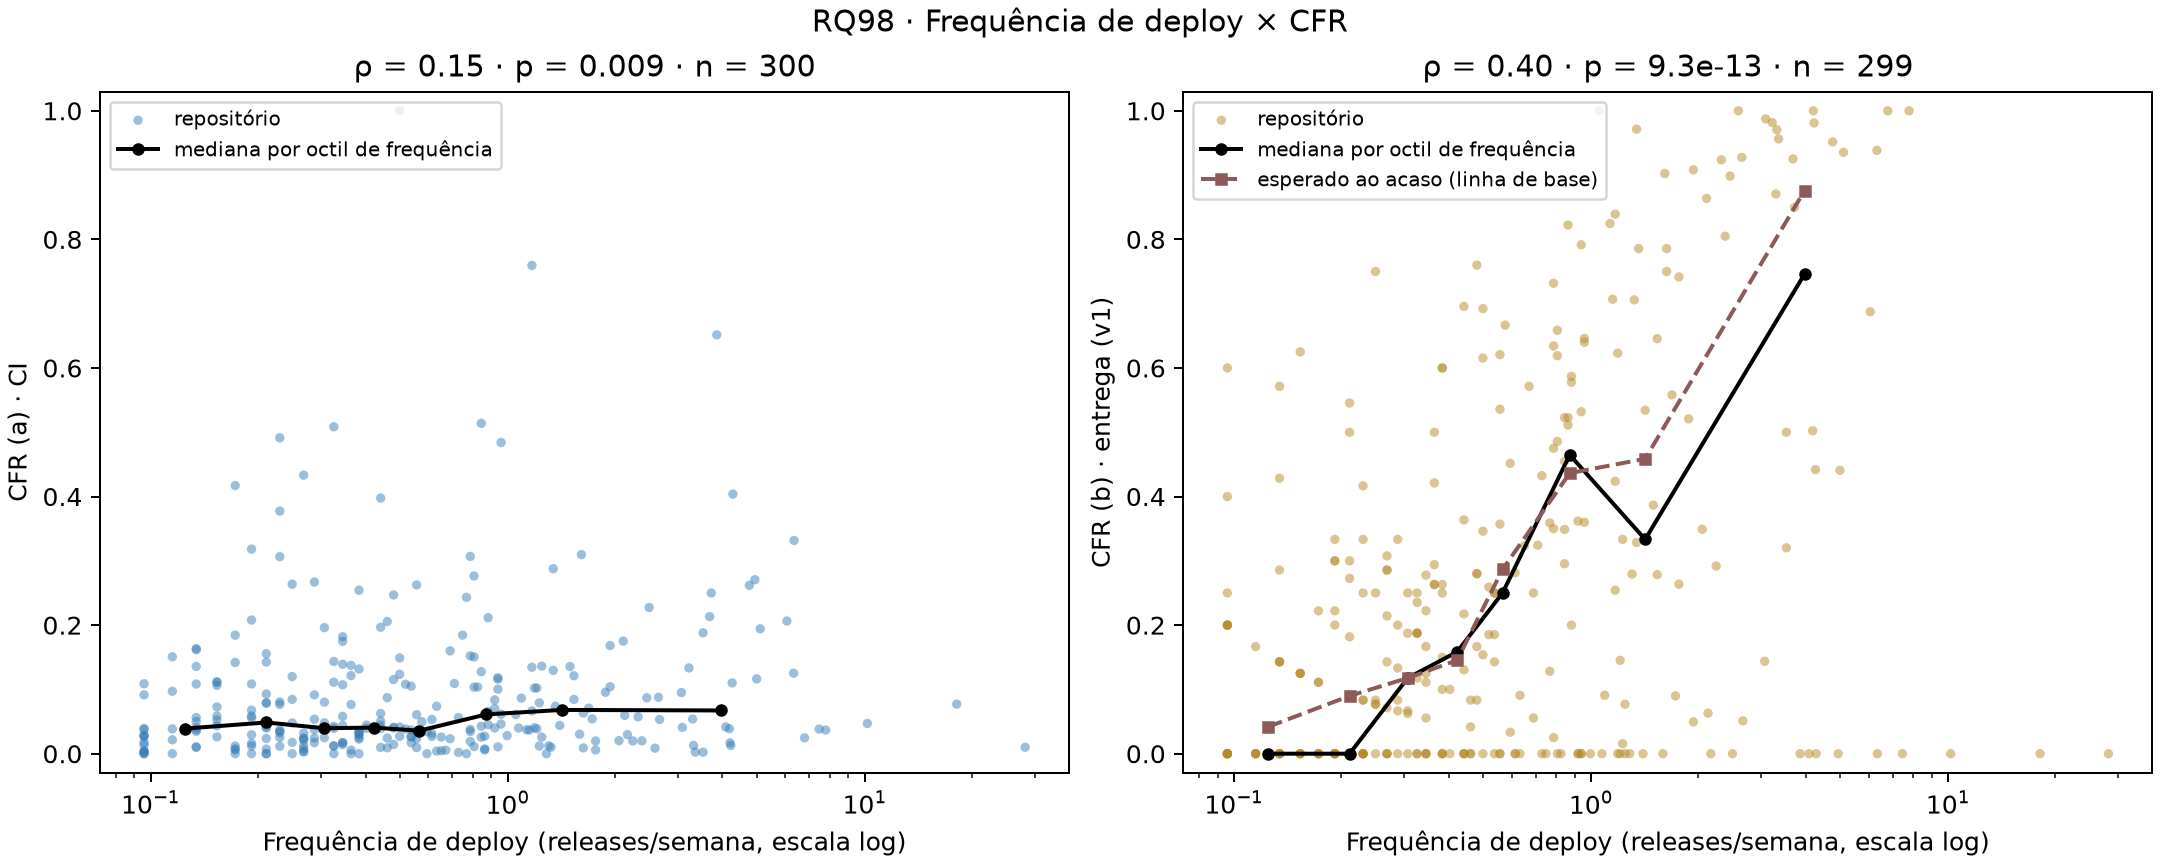
\includegraphics[width=0.95\linewidth]{figuras/dispersao_df_cfr.png}
\caption{Frequência de deploy (escala logarítmica) e CFR. Linha preta: mediana por octil de
frequência; linha tracejada: CFR (b) esperado ao acaso (linha de base da Seção~\ref{sec:discussao}).}
\label{fig:rq05}
\end{figure}

\subsection{RQ06 --- Características dos repositórios}
\label{sec:rq06}

\apreencher{resultados da RQ06 (issue \#93): Kruskal-Wallis ou Mann-Whitney por fator, p-valores
com correção de Holm, $\varepsilon^2$ e $\delta$ de Cliff}

\subsection{RQ07 --- Sensibilidade da classificação DORA}

Classificamos cada repositório em sete combinações de definições (C1 a C7, Tabela~\ref{tab:rq07}).
Dos 279 repositórios classificados em todas elas, 163 (58,4\%) têm a mesma classe geral em todas
e 116 (41,6\%) mudam em pelo menos uma alternativa à C1. Trocar só a unidade de deploy (C5 e C6)
muda de 3,6\% a 10,7\% das classes, sempre para melhor ($\kappa$ de 0,85 a 0,95); as
combinações com o CFR (b) mudam de 20,8\% a 35,5\%, e 75\% das mudanças são para pior. No nível
de cada métrica, trocar o CFR (a) pelo (b) muda a classe de 57,2\% dos repositórios
($\kappa = 0{,}02$), o \textit{lead time} (a) pelo (b), de 42,3\%, e a unidade de deploy de
release para tag, de 24,0\%.

\begin{table}[ht]
\centering
\small
\caption{Mudança da classe geral em relação à C1 (279 a 280 repositórios por par).}
\label{tab:rq07}
\begin{tabular}{llrrl}
\hline
Combinação & O que muda em relação à C1 & Mudam (\%) & $\kappa$ pond. & Landis--Koch \\
\hline
C2 & \textit{lead time} (b)                     & 14,3 & 0,79 & substancial \\
C3 & CFR (b)                                    & 20,8 & 0,68 & substancial \\
C4 & \textit{lead time} (b) e CFR (b)           & 29,7 & 0,52 & moderada \\
C5 & pré-releases contam como deploy            & 3,6  & 0,95 & quase perfeita \\
C6 & tags contam como deploy                    & 10,7 & 0,85 & quase perfeita \\
C7 & tags, \textit{lead time} (b) e CFR (b)     & 35,5 & 0,44 & moderada \\
\hline
\end{tabular}
\end{table}
 depois de % Secao 2 do artigo do LAB03 (template SBC). Issue #90.
% Uso no Overleaf: \input{metodologia} depois de \input{introducao}.
% Requer os mesmos pacotes da introducao (nada alem do template).
%
% Trechos entre \apreencher{...} dependem de dados que ainda nao existem (amostra
% final de 300, rotulos humanos, consenso, F1) ou de confirmacao do professor
% (janela oficial). Nao ha numero inventado: o funil e o piloto da Sprint 01 sao
% identificados como tais. Busque por "apreencher" antes de entregar.

\providecommand{\apreencher}[1]{\textbf{[a preencher: #1]}}

\section{Metodologia}
\label{sec:metodologia}

\subsection{Visão geral}

O estudo calcula as quatro métricas DORA, a partir de dados públicos do GitHub,
para repositórios \textit{open-source} populares que usam GitHub Actions, e mede
a confiabilidade dessas medidas por duas vias: a validação manual das
heurísticas (Seção~\ref{sec:validacao}) e a análise de sensibilidade às
definições operacionais (RQ07). Todas as definições abaixo são comuns à turma,
para que os resultados sejam comparáveis e o pipeline possa ser replicado por
outro grupo (Seção~6).

\subsection{Fonte de dados e coleta}
\label{sec:coleta}

A coleta usa um cliente próprio das APIs REST e GraphQL do GitHub, sem
bibliotecas de acesso à API. A busca de candidatos (\texttt{GET
/search/repositories}) é fatiada por faixas de estrelas para contornar o teto de
1.000 resultados por consulta, e reúne 8.000 candidatos. Os metadados de cada
um (estrelas, linguagem principal, data de criação, \textit{default branch},
indicadores de \textit{fork}, arquivamento e repositório vazio) vêm da API
GraphQL. Para os repositórios aceitos, o pipeline coleta, pela API REST, as
releases (\texttt{/releases}), os \textit{commits} entre releases consecutivas
(\texttt{/compare}, com paginação para ultrapassar o limite de 250 \textit{commits}),
as tags e as execuções de \textit{workflow} (\texttt{/actions/runs}) do
\textit{default branch}.

Duas decisões de coleta afetam a validade. Primeiro, a busca de execuções
retorna no máximo 1.000 resultados por consulta; por isso a janela é consultada
mês a mês e qualquer intervalo que atinja o teto é dividido ao meio (até o
nível de segundos), de modo que nenhuma execução se perde sem aviso. Segundo, o
pipeline descarta repositórios com mais de 20.000 execuções na janela, por custo
de coleta; esse limite é contabilizado no funil e discutido como limitação.

A coleta é um pipeline reprodutível, executado por um único comando. Toda
resposta da API é gravada em disco (um arquivo por URL), o que permite retomar
uma coleta interrompida sem repetir chamadas. O cliente lê os cabeçalhos
\texttt{X-RateLimit-Remaining} e \texttt{X-RateLimit-Reset} e espera
sozinho quando a cota acaba. Erros temporários (respostas 5xx e quedas de rede)
são repetidos com \textit{backoff} exponencial (1~s, 2~s, 4~s, \ldots, até 60~s,
em até 6 tentativas). O \textit{token} vem de variável de ambiente e nunca é
versionado. As funções que calculam as métricas têm testes automatizados
(\textit{pytest}, cobertura mínima de 80\% do módulo de métricas, medida com
\textit{pytest-cov}) executados no GitHub Actions do grupo a cada \textit{push}.

\subsection{Seleção da amostra e funil}
\label{sec:funil}

Os candidatos são avaliados em ordem decrescente de estrelas, do critério mais
barato ao mais caro, até se atingir a meta de pelo menos 300 repositórios. Um
repositório entra na amostra se (i) não é \textit{fork}, está ativo (não
arquivado, desabilitado ou vazio) e tem \textit{default branch}; (ii) usa GitHub
Actions (\texttt{total\_count > 0} em \texttt{/actions/workflows}); (iii) tem
pelo menos 5 releases publicadas na janela; e (iv) tem pelo menos 50 execuções
válidas no \textit{default branch} na janela. Os critérios não são relaxados para
atingir a meta. A Tabela~\ref{tab:funil} mostra o funil; as colunas trazem o
piloto da primeira sprint (meta de 100) e a amostra final.

\begin{table}[ht]
\centering
\small
\caption{Funil de seleção. O piloto (Sprint 01) foi coletado com a janela
provisória; a amostra final ainda não foi exportada.}
\label{tab:funil}
\begin{tabular}{lrr}
\hline
Etapa & Piloto ($n=100$) & Final \\
\hline
Candidatos com metadados & 8.000 & \apreencher{n} \\
Ativos (sem \textit{fork}/arquivados/vazios) & 7.519 & \apreencher{n} \\
Avaliados até a meta & 272 & \apreencher{n} \\
Usam GitHub Actions & 253 & \apreencher{n} \\
$\geq 5$ releases na janela & 132 & \apreencher{n} \\
$\leq 20.000$ execuções (custo) & 114 & \apreencher{n} \\
$\geq 50$ execuções válidas & 100 & \apreencher{$\geq 300$} \\
\hline
\end{tabular}
\end{table}

\subsection{Definições operacionais}
\label{sec:definicoes}

\begin{table}[ht]
\centering
\small
\caption{Definições operacionais comuns à turma.}
\label{tab:definicoes}
\begin{tabular}{p{0.22\linewidth}p{0.68\linewidth}}
\hline
Elemento & Definição \\
\hline
Janela & 12 meses, de 01/10/2025 a 30/09/2026, com as duas datas inclusivas
\apreencher{confirmar a janela oficial com o professor} \\
\textit{Branch} & Apenas o \textit{default branch} (\texttt{default\_branch}) \\
Deploy & Release publicada (\texttt{draft = false}) e não pré-release;
pré-releases e tags são variantes da RQ07 \\
Data do \textit{commit} & \texttt{commit.author.date} \\
Execução de CI & \textit{Workflow run} do \textit{default branch} com
\texttt{event = push}, criado na janela \\
Sucesso & \texttt{success} \\
Falha & \texttt{failure}, \texttt{timed\_out}, \texttt{startup\_failure} \\
Ignorada & \texttt{cancelled}, \texttt{skipped}, \texttt{neutral},
\texttt{action\_required}, \texttt{stale} ou vazio \\
Censura & Evento final não observado na janela: registrado como censurado, não
descartado \\
\hline
\end{tabular}
\end{table}

\subsection{Métricas e variantes}
\label{sec:metricas}

Em todas as RQs reportamos mediana e intervalo interquartil (IQR, quartis por
interpolação linear), e não média e desvio-padrão, porque as distribuições são
assimétricas.

\textbf{RQ01 -- Frequência de deploy.} Releases publicadas na janela divididas
pelo número de semanas da janela ($\approx 52{,}1$).

\textbf{RQ02 -- \textit{Lead time}.} Para cada release R da janela, os
\textit{commits} são os do \texttt{compare} com a release publicada
imediatamente anterior, que pode estar fora da janela. Na variante (a), o
\textit{lead time} de R é a data de R menos a do \textit{commit} mais antigo, e o
valor do repositório é a mediana entre as releases. Na variante (b), cada
\textit{commit} contribui com a data de R menos a sua, e o valor do repositório é
a mediana de todos os \textit{commits} de todas as releases (e não uma mediana de
medianas). Decisões do grupo: a primeira release da história do repositório é
ignorada; \texttt{compare} indisponível (por exemplo, tag apagada) ou truncado
exclui a release do cálculo e é contado; uma release sem \textit{commits} novos
fica fora das duas variantes; e um \textit{commit} com data de autoria posterior
à da release (relógio errado ou tag movida) é descartado e contado.

\textbf{RQ03 -- Taxa de falha (CFR).} A variante (a), de CI, é o número de
execuções com falha dividido por falhas mais sucessos, considerando todos os
\textit{workflows} juntos; ela mede falha de pipeline, não de produção. A
variante (b), de entrega, considera uma release R como falha se for seguida, em
até 7 dias (inclusive), por uma release corretiva; o CFR é o número de releases
que falharam dividido pelo de avaliadas. Várias corretivas na semana não
multiplicam a falha de R. Releases dos últimos 7 dias da janela são censuradas e
ficam fora do denominador.

\textbf{RQ04 -- Tempo de recuperação.} Dentro de cada \textit{workflow}, um
episódio de falha começa na primeira falha após um sucesso e termina no próximo
sucesso; sua duração é o \texttt{updated\_at} do sucesso menos o
\texttt{run\_started\_at} da falha. Execuções ignoradas não interrompem nem
iniciam episódios. O valor do repositório é a mediana dos episódios de todos os
seus \textit{workflows}. Episódios sem sucesso até o fim da janela são
censurados à direita. Por decisão do grupo, também são censurados (à esquerda)
os episódios de um \textit{workflow} cuja primeira execução válida na janela já
é uma falha, pois o início real é desconhecido. Episódios censurados não entram
na mediana, e a proporção deles é reportada por repositório. Repositório sem
falhas tem recuperação indefinida (e não zero).

\textbf{Classificação DORA.} Cada métrica recebe 4 (Elite), 3 (High), 2 (Medium)
ou 1 (Low) pelos cortes fixos da disciplina; a categoria geral é a mediana dos
quatro valores, arredondada para baixo.

\subsection{Heurística de release corretiva}
\label{sec:heuristica}

Uma release é corretiva quando seu objetivo principal é corrigir um defeito
recente. Como o GitHub não registra isso, usamos heurísticas sobre a tag e sobre
a primeira linha das mensagens dos \textit{commits} entre a release anterior e a
avaliada. Testamos três versões, aplicadas sempre em relação à release publicada
imediatamente anterior:

\begin{itemize}
  \item \textbf{v1 (\textit{patch} SemVer):} só o número de \textit{patch}
  mudou (por exemplo, $2.3.0 \rightarrow 2.3.1$). Tags que não seguem SemVer
  estrito, pré-releases e \textit{downgrades} nunca são corretivas.
  \item \textbf{v2 (\textit{patch} ou mensagem):} v1, ou algum \textit{commit}
  com \texttt{revert}, \texttt{hotfix} ou \texttt{fix}.
  \item \textbf{v3 (correção de defeito):} \texttt{revert} ou \texttt{hotfix}
  bastam; caso contrário, exige \textit{commit} \texttt{fix} que não trate de
  \textit{typo}, documentação, CI, testes ou dependências, e que o \textit{patch}
  tenha mudado ou que ao menos metade dos \textit{commits} (sem \textit{merges}) seja
  correção, sem \textit{commit} de funcionalidade. Sem mensagens disponíveis,
  vale só a tag.
\end{itemize}

A versão usada no CFR (b) é a que atingir F1~$\geq 0{,}70$ contra o consenso
da amostra-ouro; se nenhuma atingir, a heurística é refinada e reavaliada, e
todas as versões e seus F1 são reportadas. Resultados:
\apreencher{P, R e F1 de v1, v2, v3 e das versões seguintes}.
As heurísticas não leem as \textit{release notes} nem o \textit{diff}; isso é
uma limitação.

\subsection{Validação manual (amostra-ouro)}
\label{sec:validacao}

Sorteamos 60 repositórios da amostra final com \texttt{df.sample(n=60,
random\_state=42)}, sobre a amostra ordenada por nome (a ordem do arquivo não
altera o sorteio), e, em cada um, até 5 releases da definição principal de
deploy que tenham release anterior (a primeira da história fica de fora, pois
não há lista de \textit{commits} para ler). Os três integrantes rotularam, de
forma independente, sem consultar os demais e sem ver a saída da heurística, em
planilhas idênticas com ligações para a página da release e para o
\texttt{compare}: (i)~o tipo do projeto (biblioteca/\textit{framework},
aplicação/serviço, ferramenta CLI ou outro); (ii)~se as releases representam
entregas reais ao usuário (sim, não ou incerto); e (iii)~se cada release
sorteada é corretiva (sim ou não).

A concordância entre os três avaliadores é medida com o $\kappa$ de Fleiss em
cada dimensão (interpretação de Landis e Koch). Os casos divergentes são
discutidos pelo grupo e geram o rótulo de consenso; o protocolo de desempate é
\apreencher{protocolo definido na consolidação do consenso}. Um $\kappa$ baixo é
tratado como achado sobre a ambiguidade do critério. A heurística é avaliada
contra o consenso com precisão, \textit{recall} e F1 (classe positiva:
corretiva). Como as regras são ajustadas olhando os erros desta mesma amostra, o
F1 final tende a ser otimista. Resultados: \apreencher{$\kappa$ por dimensão,
tamanho do consenso}. O tipo do projeto rotulado alimenta a RQ06.

\subsection{Análise estatística}
\label{sec:analise}

Para a RQ05, usamos a correlação de Spearman ($\rho$, p-valor e $n$) entre a
frequência de deploy e o CFR, separadamente para as variantes (a) e (b). Na RQ06,
comparamos as métricas entre subgrupos de pelo menos três fatores (linguagem,
quartis de estrelas, de contribuidores e de idade, e tipo do projeto) com
Kruskal-Wallis (ou Mann-Whitney, quando há dois grupos), corrigimos os p-valores
por Holm e reportamos o tamanho de efeito ($\varepsilon^2 = H/(n-1)$ ou
$\delta$ de Cliff). Na RQ07, montamos ao menos três combinações de definições
(por exemplo, release, release com pré-release e tag como unidade de deploy,
combinadas com as variantes de \textit{lead time} e de CFR), classificamos cada
repositório em cada combinação e calculamos, por par, a proporção que muda de
categoria e o $\kappa$ de Cohen ponderado (pesos lineares).

\subsection{Disponibilidade}

O código, os testes, o dicionário de dados e os CSVs finais estão no
repositório do grupo (Seção~7). O pipeline é executável por outro grupo com um
único comando, conforme o README.
; as figuras ficam em figuras/
% (\usepackage{graphicx}, ja no template).
%
% Todos os numeros vem das analises do repositorio (entregas/laboratorio-03/sprint-03):
% RQ91 (RQ01), RQ94 (RQ02), RQ97 (RQ03), RQ92 (RQ04), RQ95 (classificacao C1),
% RQ98 (RQ05), RQ96 (RQ07). Janela provisoria; CFR (b) com a heuristica v1, ainda sem F1 medido.
% Trechos em \apreencher{...} dependem de analises ainda nao feitas (RQ06, issue #93) ou da
% validacao manual (issues #85 a #89). Busque por "apreencher" antes de entregar.

\providecommand{\apreencher}[1]{\textbf{[a preencher: #1]}}

\section{Resultados}
\label{sec:resultados}

Os resultados se referem aos 300 repositórios da amostra final (Seção~\ref{sec:funil}),
na janela de 01/10/2025 a 30/09/2026, ainda provisória (Seção~\ref{sec:definicoes}). Cada
repositório tem o mesmo peso e a estatística da amostra é a mediana dos valores dos
repositórios, com o intervalo interquartil (IQR, Q1--Q3). A Tabela~\ref{tab:descritivo} resume
as métricas e a classificação DORA de cada uma. Nas Seções~\ref{sec:rq03} e~\ref{sec:rq05},
o CFR (b) usa a versão v1 da heurística de release corretiva, que ainda não tem F1 medido
contra o consenso da amostra-ouro (\apreencher{P, R e F1 das versões v1, v2 e v3}).

\begin{table}[ht]
\centering
\small
\caption{Métricas DORA e classes (\% dos repositórios com a métrica definida). Frequência em
releases/semana; \textit{lead time} em dias; CFR em \%; recuperação em horas.}
\label{tab:descritivo}
\begin{tabular}{lrrrrrr}
\hline
Métrica & $n$ & Mediana (Q1--Q3) & Elite & High & Medium & Low \\
\hline
Frequência de deploy      & 300 & 0,48 (0,23--1,16) & 1,7  & 25,0 & 50,7 & 22,7 \\
\textit{Lead time} (a)    & 300 & 10,5 (3,6--39,5)  & 14,3 & 25,0 & 30,3 & 30,3 \\
\textit{Lead time} (b)    & 300 & 12,1 (3,3--57,5)  & 10,3 & 28,7 & 28,7 & 32,3 \\
CFR (a), CI               & 300 & 4,6 (2,3--11,1)   & 83,0 & 11,3 & 3,3  & 2,3  \\
CFR (b), entrega (v1)     & 299 & 18,8 (0,0--44,7)  & 47,5 & 18,4 & 9,0  & 25,1 \\
Recuperação               & 280 & 2,7 (1,1--6,9)    & 23,2 & 66,4 & 9,3  & 1,1  \\
\hline
Classe geral (C1)         & 280 & ---               & 6,4  & 43,6 & 45,7 & 4,3  \\
\hline
\end{tabular}
\end{table}

\begin{figure}[ht]
\centering
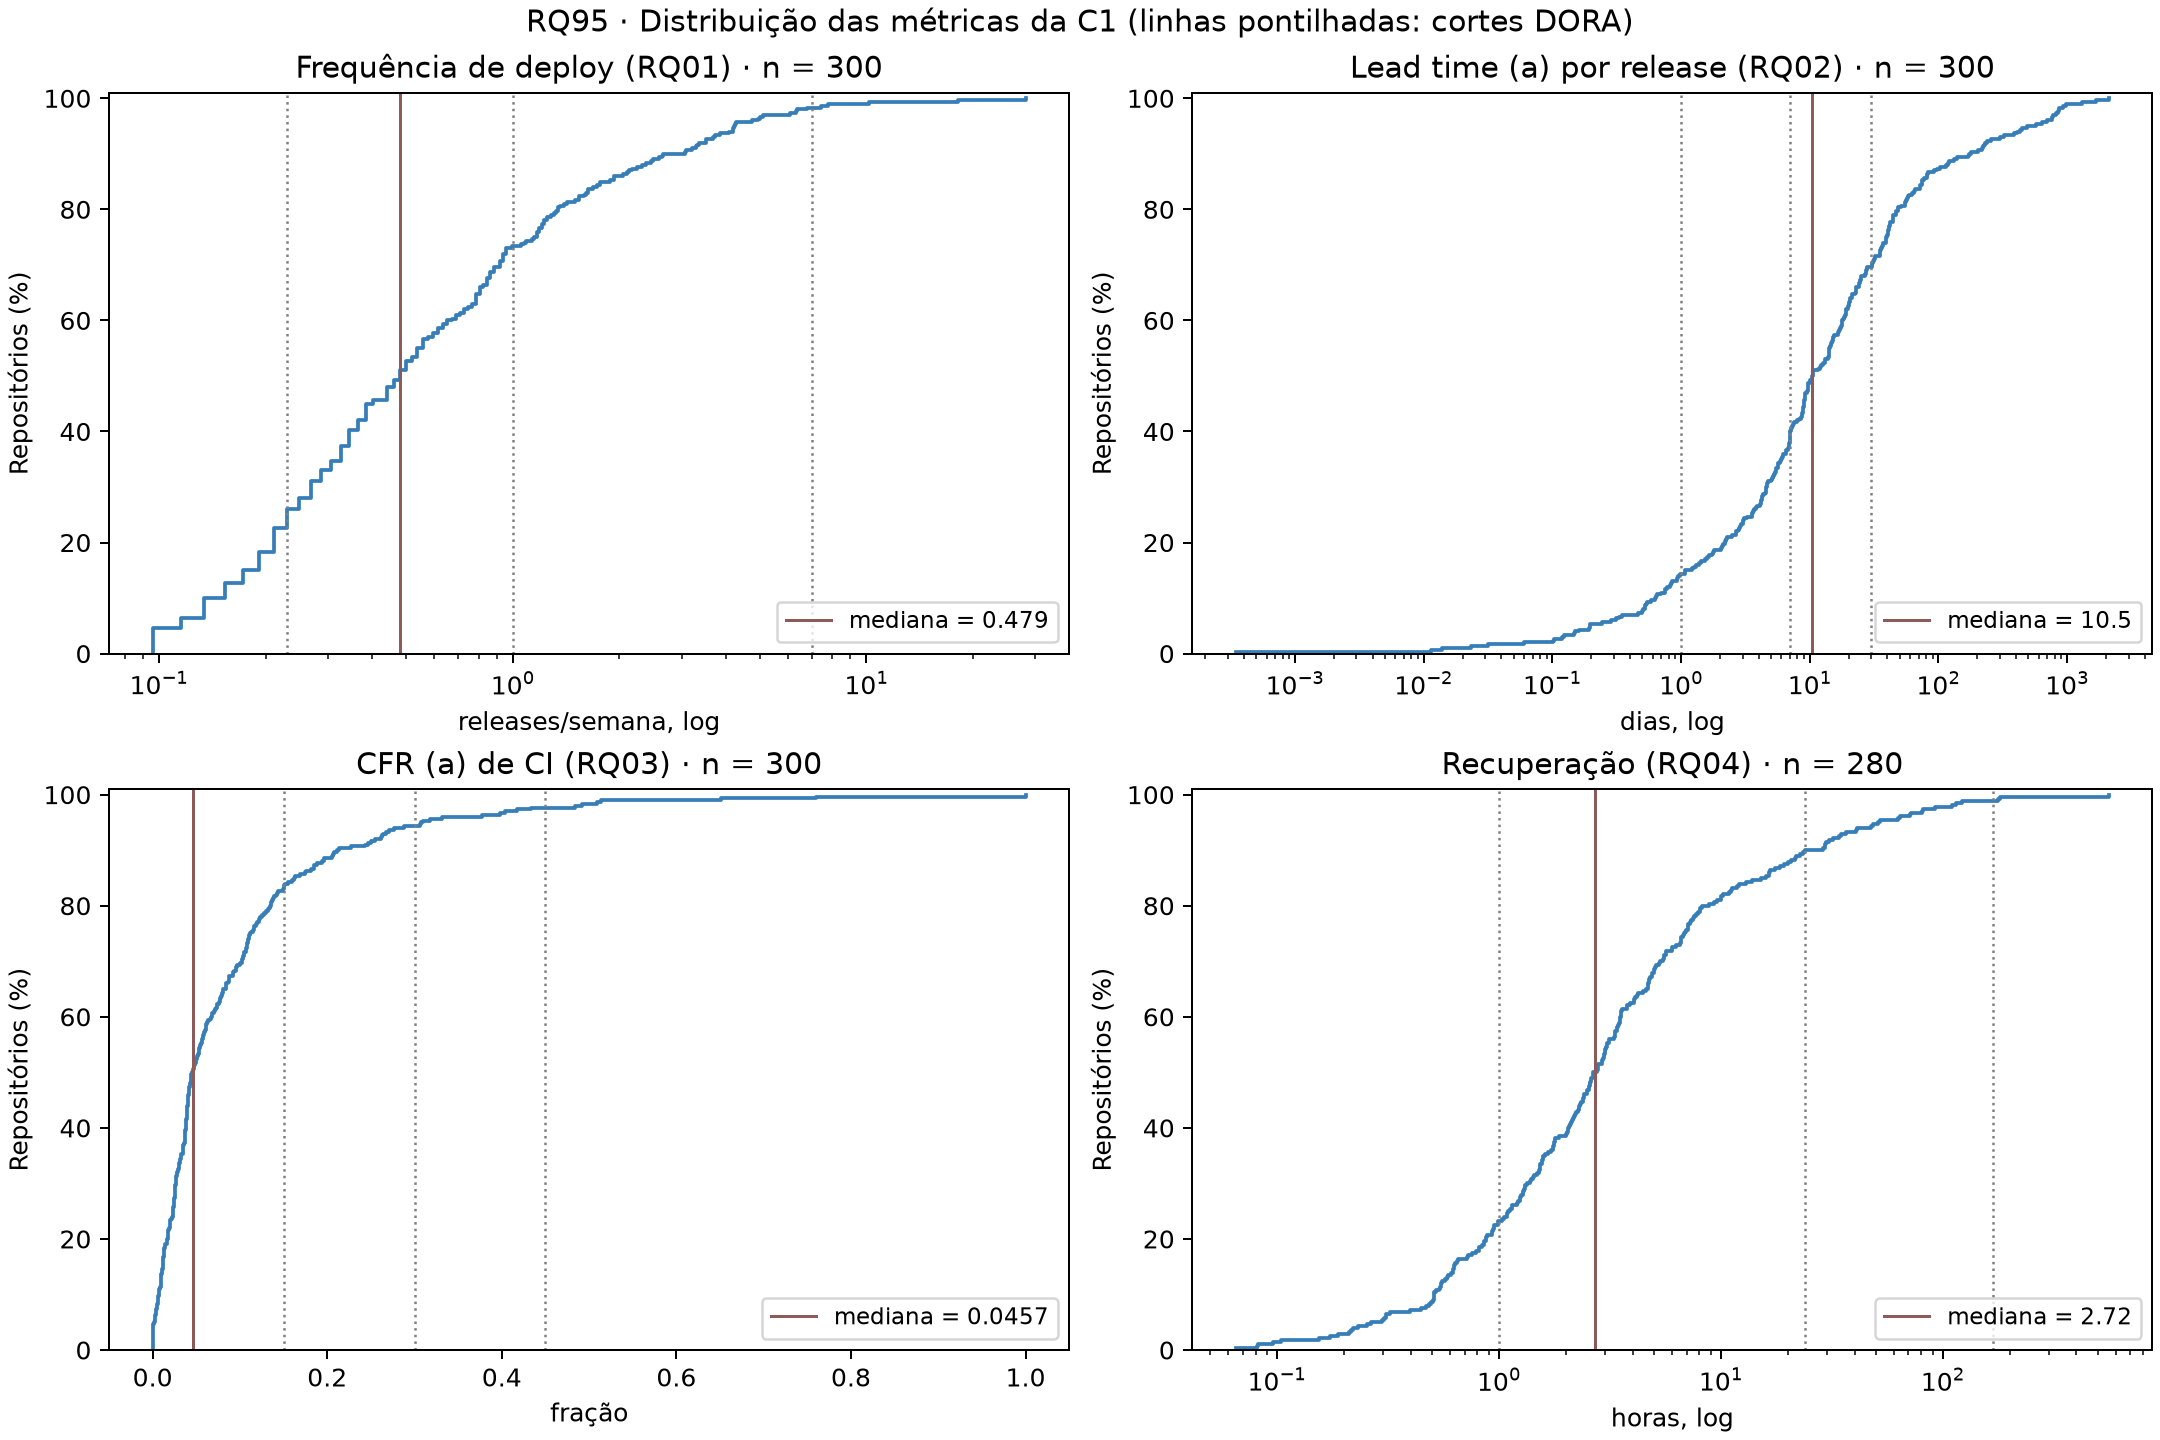
\includegraphics[width=0.92\linewidth]{figuras/distribuicoes_c1.png}
\caption{Distribuição acumulada das métricas da combinação C1 (linhas pontilhadas: cortes DORA;
linha vermelha: mediana).}
\label{fig:distribuicoes}
\end{figure}

\subsection{RQ01 --- Frequência de deploy}

A mediana é de 0,48 release/semana (IQR 0,93), com cauda longa à direita: o máximo é de 28,2
releases/semana e 33 repositórios passam do limite de Tukey (2,54). Os 30 repositórios mais
ativos (10\%) concentram 51,5\% das releases. Metade dos repositórios é Medium (50,7\%), um quarto é
High e só 5 (1,7\%) são Elite.

\subsection{RQ02 --- \textit{Lead time}}

Por release (a), a mediana é de 10,5 dias (IQR 35,9); por \textit{commit} (b), 12,1 dias (IQR 54,3).
Das 18.206 releases da janela, 14.589 têm \textit{lead time}; as demais são a primeira release
da história do repositório (57) ou não trazem \textit{commits} novos (3.560). A variante (b) é
menor que a (a) em 177 repositórios e maior em 122; a razão (b)/(a) tem mediana de 0,78 e o
teste de Wilcoxon pareado não rejeita a igualdade ($p = 0{,}12$). Trocar (a) por (b) muda a classe de
127 repositórios (42,3\%). Quanto maior a release, menor o (b) em relação ao (a)
($\rho = -0{,}30$ entre o número de \textit{commits} por release e a razão (b)/(a)).

\subsection{RQ03 --- Taxa de falha das mudanças}
\label{sec:rq03}

O CFR de CI (a) tem mediana de 4,6\% (IQR 8,8 pontos percentuais): 83,0\% dos repositórios são
Elite, e só 14 não têm nenhuma falha. O CFR de entrega (b), com a v1, tem mediana de 18,8\%
(IQR 44,7 pontos), muito mais disperso, e espalha os repositórios pelas quatro classes
(Tabela~\ref{tab:descritivo}). Somando todos os \textit{runs} e todas as releases, o CFR é de
9,2\% (a) e de 38,2\% (b). As duas variantes quase não concordam: $\rho = 0{,}07$ entre elas
($p = 0{,}26$), o (b) é maior que o (a) em 182 de 299 repositórios (Wilcoxon, $p < 10^{-15}$)
e 57,2\% dos repositórios mudam de classe ao trocar uma pela outra
($\kappa$ ponderado $= 0{,}02$, concordância leve), 144 deles para pior.

Os dois proxies medem coisas diferentes. No (a), 98,6\% das falhas são \texttt{failure} e 1,4\%
são \texttt{startup\_failure}, e o workflow que mais falha em cada repositório responde, na
mediana, por 73,1\% das falhas: o CFR (a) reflete sobretudo um ou dois \textit{workflows}. No
(b), 39,2\% das releases (7.130 de 18.206) têm tag fora do SemVer estrito e nunca são
corretivas na v1; 42 repositórios não têm nenhuma tag SemVer, e o CFR (b) deles é zero por
construção. Por outro lado, na mediana 42,9\% das releases de um repositório mudam só o
\textit{patch}. O nível do (b) depende da heurística: com as versões v2 (\textit{patch} ou qualquer
\textit{commit} com \texttt{fix}, \texttt{revert} ou \texttt{hotfix}) e v3 (correção de defeito),
a mediana vai a 43,5\% e 27,3\%, e 40,8\% e 31,8\% dos repositórios mudam de classe em relação à
v1. A v2 e a v3 marcam como corretivas 98,6\% e 61,3\% das releases na mediana, o que indica
excesso de marcações.

\begin{figure}[ht]
\centering
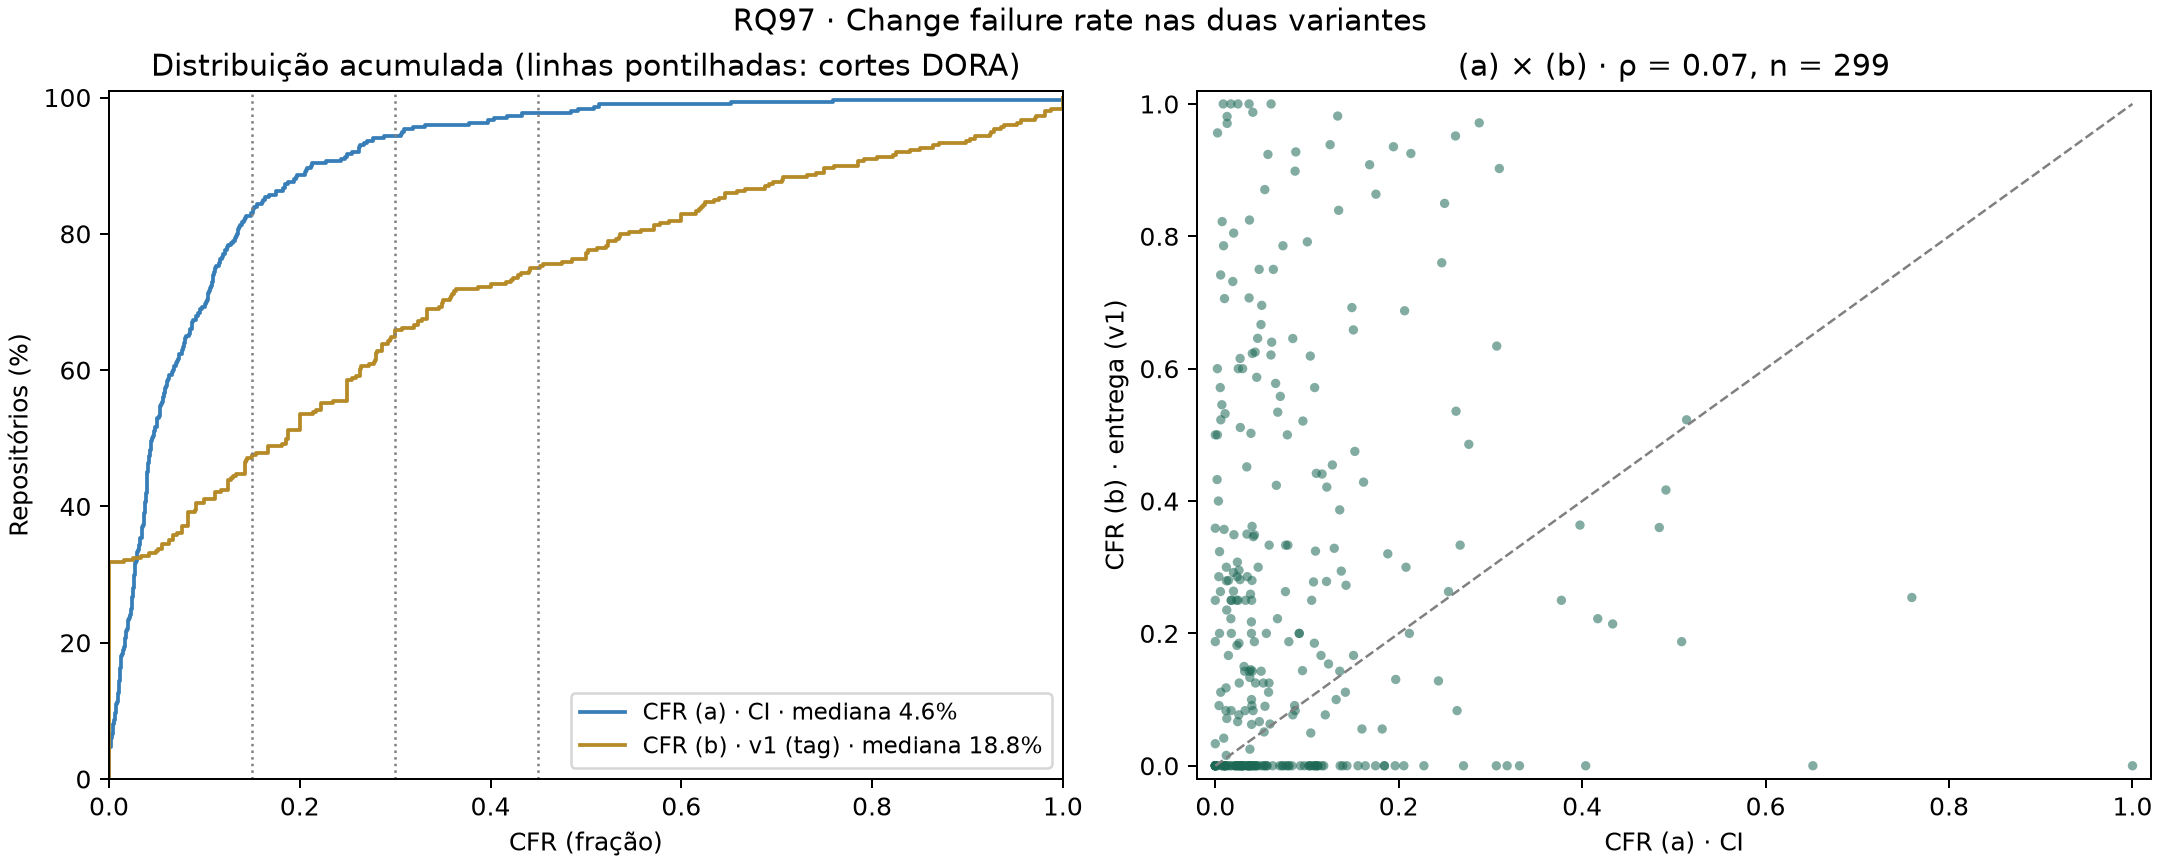
\includegraphics[width=0.95\linewidth]{figuras/cfr_variantes.png}
\caption{CFR nas duas variantes: distribuição acumulada (esquerda) e dispersão (a)~$\times$~(b)
(direita); linha tracejada: $y = x$.}
\label{fig:cfr}
\end{figure}

\subsection{RQ04 --- Tempo de recuperação}

Há 280 repositórios com tempo estimável (20 não têm nenhum episódio de falha completo e ficam
sem estimativa, não com zero). A mediana é de 2,7 horas (IQR 5,7), com cauda longa: o P90 é de
24,5 horas e o máximo, de 560 horas. Dos 27.839 episódios, 230 (0,83\%) terminam censurados à
direita, mas 24 repositórios têm pelo menos 10\% dos episódios censurados. Em 88,9\% dos
episódios a recuperação ocorre em até 24 horas (79,2\% com peso igual por repositório).

\subsection{Classificação DORA geral}

Pela combinação de referência C1 (release, \textit{lead time} (a), CFR (a)), 280 repositórios
recebem classe geral: 6,4\% Elite, 43,6\% High, 45,7\% Medium e 4,3\% Low; os 20 repositórios sem
episódio de falha completo ficam sem classe. A estabilidade é alta (Elite ou High nas duas métricas
da dimensão) em 85,4\% dos repositórios classificados, mas só 21,1\% têm velocidade alta. A classe
geral é limitada pela velocidade, não pela estabilidade.

\subsection{RQ05 --- Frequência de deploy e CFR}
\label{sec:rq05}

\begin{table}[ht]
\centering
\small
\caption{Correlação de Spearman entre a frequência de deploy e o CFR (IC de 95\% por
\textit{bootstrap}; $p$ com correção de Holm). O $\rho$ parcial controla idade e contribuidores
no (a) e o CFR (b) esperado ao acaso no (b) (Seção~\ref{sec:discussao}).}
\label{tab:rq05}
\begin{tabular}{lrrrrr}
\hline
Variante & $n$ & $\rho$ & $p$ (Holm) & IC 95\% & $\rho$ parcial \\
\hline
CFR (a), CI           & 300 & 0,15 & 0,009            & 0,04 a 0,27 & 0,09 ($p = 0{,}14$) \\
CFR (b), entrega (v1) & 299 & 0,40 & $2 \times 10^{-12}$ & 0,29 a 0,51 & $-0{,}16$ ($p = 0{,}005$) \\
\hline
\end{tabular}
\end{table}

A frequência de deploy tem correlação fraca e positiva com o CFR (a) e moderada e positiva com o CFR (b)
(Tabela~\ref{tab:rq05}, Figura~\ref{fig:rq05}). Em quartis de frequência, a mediana do CFR (a) fica
em torno de 4--7\% em todas as faixas, enquanto a do CFR (b) sobe de 0\% (Q1) para 44,2\% (Q4).
Em termos de classes, 94\% dos repositórios de frequência alta (Elite ou High) têm CFR (a) Elite
ou High, contra 95\% dos de frequência baixa (Fisher, $p = 0{,}78$); no CFR (b), 40\% contra 75\%
($p < 10^{-7}$).

\begin{figure}[ht]
\centering
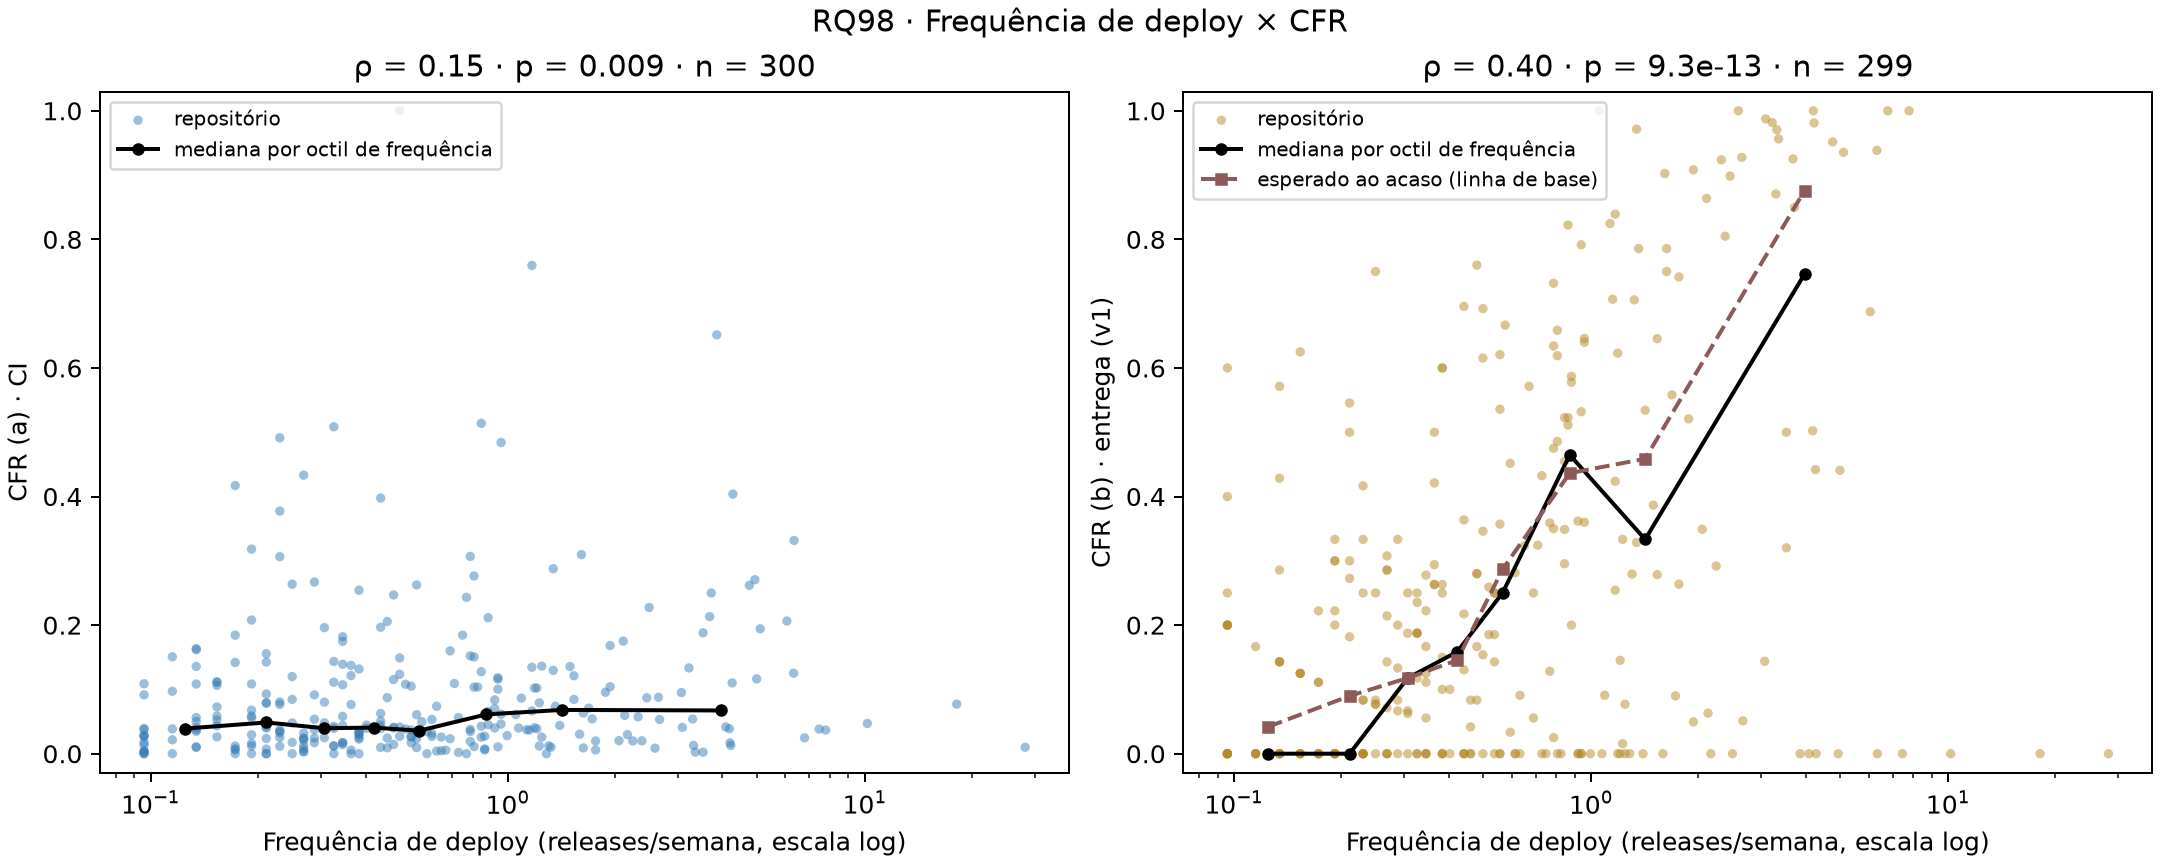
\includegraphics[width=0.95\linewidth]{figuras/dispersao_df_cfr.png}
\caption{Frequência de deploy (escala logarítmica) e CFR. Linha preta: mediana por octil de
frequência; linha tracejada: CFR (b) esperado ao acaso (linha de base da Seção~\ref{sec:discussao}).}
\label{fig:rq05}
\end{figure}

\subsection{RQ06 --- Características dos repositórios}
\label{sec:rq06}

\apreencher{resultados da RQ06 (issue \#93): Kruskal-Wallis ou Mann-Whitney por fator, p-valores
com correção de Holm, $\varepsilon^2$ e $\delta$ de Cliff}

\subsection{RQ07 --- Sensibilidade da classificação DORA}

Classificamos cada repositório em sete combinações de definições (C1 a C7, Tabela~\ref{tab:rq07}).
Dos 279 repositórios classificados em todas elas, 163 (58,4\%) têm a mesma classe geral em todas
e 116 (41,6\%) mudam em pelo menos uma alternativa à C1. Trocar só a unidade de deploy (C5 e C6)
muda de 3,6\% a 10,7\% das classes, sempre para melhor ($\kappa$ de 0,85 a 0,95); as
combinações com o CFR (b) mudam de 20,8\% a 35,5\%, e 75\% das mudanças são para pior. No nível
de cada métrica, trocar o CFR (a) pelo (b) muda a classe de 57,2\% dos repositórios
($\kappa = 0{,}02$), o \textit{lead time} (a) pelo (b), de 42,3\%, e a unidade de deploy de
release para tag, de 24,0\%.

\begin{table}[ht]
\centering
\small
\caption{Mudança da classe geral em relação à C1 (279 a 280 repositórios por par).}
\label{tab:rq07}
\begin{tabular}{llrrl}
\hline
Combinação & O que muda em relação à C1 & Mudam (\%) & $\kappa$ pond. & Landis--Koch \\
\hline
C2 & \textit{lead time} (b)                     & 14,3 & 0,79 & substancial \\
C3 & CFR (b)                                    & 20,8 & 0,68 & substancial \\
C4 & \textit{lead time} (b) e CFR (b)           & 29,7 & 0,52 & moderada \\
C5 & pré-releases contam como deploy            & 3,6  & 0,95 & quase perfeita \\
C6 & tags contam como deploy                    & 10,7 & 0,85 & quase perfeita \\
C7 & tags, \textit{lead time} (b) e CFR (b)     & 35,5 & 0,44 & moderada \\
\hline
\end{tabular}
\end{table}
.
% Os numeros vem das mesmas analises da Secao 3 (entregas/laboratorio-03/sprint-03, RQ91 a RQ98).
% Trechos em \apreencher{...} dependem da RQ06 (issue #93) e da validacao manual (issues #85 a #89).

\providecommand{\apreencher}[1]{\textbf{[a preencher: #1]}}

\section{Discussão}
\label{sec:discussao}

\subsection{Hipóteses e resultados}

A Tabela~\ref{tab:hipoteses} confronta cada hipótese informal da Seção~\ref{sec:hipoteses},
registrada antes da análise, com o que encontramos. Nenhuma faixa prevista foi alterada depois
da análise.

\begin{table}[ht]
\centering
\scriptsize
\caption{Hipóteses (Seção~\ref{sec:hipoteses}) frente aos resultados (Seção~\ref{sec:resultados}).}
\label{tab:hipoteses}
\begin{tabular}{p{0.05\linewidth}p{0.28\linewidth}p{0.40\linewidth}p{0.15\linewidth}}
\hline
 & Previsão & Resultado & Veredito \\
\hline
H1 & Mediana de 0,5 a 1 release/semana; Medium e High; cauda longa; poucos Elite
   & Mediana de 0,48; Medium e High somam 75,7\%; 33 extremos; 1,7\% Elite
   & Confirmada, com a mediana pouco abaixo da faixa \\
H2 & (a) em semanas (Medium ou Low); (b) sistematicamente menor; diferença cresce com o tamanho da release
   & (a) = 10,5 dias, com 60,7\% em Medium ou Low; (b) = 12,1 dias, menor em 177 de 300 repositórios, mas
     sem diferença pareada ($p = 0{,}12$); $\rho = -0{,}30$ com o tamanho
   & Parcial: (a) e o efeito do tamanho sim; (b) menor, não \\
H3 & CFR (a) de 10 a 25\%; (b) de 5 a 15\% e mais variável; $|\rho| < 0{,}3$ entre (a) e (b)
   & (a) = 4,6\%; (b) = 18,8\%, com IQR de 44,7 contra 8,8 pontos; $\rho = 0{,}07$
   & Parcial (2 de 4): variabilidade e correlação sim; níveis, não \\
H4 & Recuperação de 1 hora a 1 dia; cauda longa; censura abaixo de 10\%
   & 2,7 horas; P90 de 24,5 horas e máximo de 560; censura de 0,83\% (24 repositórios com $\geq 10$\%)
   & Confirmada \\
H5 & $\rho$ próximo de zero ou levemente negativo no (b) e próximo de zero no (a)
   & (a) $\rho = 0{,}15$; (b) $\rho = 0{,}40$, ou $-0{,}16$ após a linha de base
   & Parcial: vale, fracamente, no (a); não vale no (b) bruto \\
H6 & Efeitos pequenos a médios; contribuidores, tipo e linguagem associados
   & \apreencher{RQ06 (issue \#93)}
   & Pendente \\
H7 & $\geq 30$\% mudam de classe; $\kappa$ de 0,2 a 0,6; pré-releases e tags inflam a frequência; \textit{lead time} (b) melhora a classe
   & 1 de 6 alternativas com $\geq 30$\% (C7: 35,5\%); $\kappa$ de 0,44 a 0,95; pré-releases e tags só melhoram a classe de frequência; (b) melhora 61 repositórios e piora 66
   & Parcial: depende de qual definição muda \\
\hline
\end{tabular}
\end{table}

\subsection{O que surpreendeu e por quê}

\textbf{A velocidade é o gargalo; a estabilidade quase nunca.} Esperávamos CFR de CI entre 10\% e
25\% e encontramos 4,6\%. Com o corte de Elite em 15\%, 83\% dos repositórios são Elite no CFR (a),
e 85,4\% têm estabilidade alta contra 21,1\% com velocidade alta. O resultado é coerente com o
perfil da amostra, projetos populares com CI madura, mas também com a natureza do proxy: o CFR (a)
mede falha de pipeline, concentrada em um ou dois \textit{workflows} (73,1\% das falhas, na mediana),
e não mede defeito que chega ao usuário. Os cortes DORA vêm de questionários com empresas; aqui o
CFR (a) discrimina pouco, e a classe geral fica presa à frequência e ao \textit{lead time}. Já a
frequência baixa tem uma leitura própria: uma biblioteca que publica uma release por mês não está
``deployando'' nada, e a classe Medium da maioria dos repositórios reflete o ritmo de publicação,
não necessariamente uma entrega lenta.

\textbf{Os dois CFR respondem a perguntas diferentes.} O CFR (b) não ficou abaixo do (a), como
previsto, e a correlação entre eles é desprezível ($\rho = 0{,}07$); 57,2\% dos repositórios mudam de
classe ao trocar um pelo outro. A previsão de que medem fenômenos distintos se confirmou, mas o
nível do (b) é frágil: depende de uma heurística cuja versão v1 deixa de fora 39,2\% das releases
(tags fora do SemVer), e a mediana vai de 18,8\% a 43,5\% conforme a versão
(Seção~\ref{sec:rq03}). Sem o F1 contra o consenso da amostra-ouro (\apreencher{P, R e F1 das versões
da heurística e $\kappa$ de Fleiss entre os avaliadores}), não sabemos qual dessas taxas se aproxima da
taxa real de releases corretivas; por isso reportamos as duas variantes e não escolhemos a mais
favorável a uma hipótese.

\textbf{Mais releases, mais CFR (b), mas por aritmética.} Esperávamos ausência de \textit{trade-off}, em
linha com o DORA. O $\rho$ bruto entre frequência e CFR (b) foi de $0{,}40$, e 40\% dos repositórios de
frequência alta têm CFR (b) Elite ou High, contra 75\% dos de frequência baixa. Lido sem cuidado, isso
sugeriria que publicar mais piora a estabilidade. Mas o CFR (b) conta uma falha quando alguma release
\textit{patch} sai em até 7 dias, e quanto mais releases, maior a chance de isso acontecer ao acaso: a fração
de releases com alguma sucessora em 7 dias tem $\rho = 0{,}83$ com a frequência, enquanto a proporção de
\textit{patches} quase não varia com ela. Embaralhando, em cada repositório, quais releases são corretivas,
o CFR (b) esperado ao acaso tem $\rho = 0{,}59$ com a frequência, acima do observado, e o $\rho$ parcial,
controlando esse esperado, é $-0{,}16$. Para o CFR (a), a relação é fraca ($\rho = 0{,}15$) e perde a
significância ao controlar idade e contribuidores ($0{,}09$; $p = 0{,}14$). Assim, os dados
\textit{open source} não confirmam nem contradizem a afirmação do DORA de que velocidade e estabilidade
andam juntas: o proxy de entrega tem um acoplamento aritmético com a frequência, e o de CI quase não
discrimina. Correlação não implica causalidade; tamanho da equipe, maturidade e automação de
releases podem afetar as duas medidas.

\textbf{\textit{Lead time} por \textit{commit} não é menor que por release.} Previmos o (b) sistematicamente
menor, porque um \textit{commit} antigo ``esquecido'' infla o (a) e é diluído no (b). O mecanismo aparece nas
releases grandes ($\rho = -0{,}30$ entre o tamanho e a razão (b)/(a)), mas o (b) pondera as releases pelo
número de \textit{commits}: onde poucas releases grandes concentram \textit{commits} antigos e muitas releases
pequenas são rápidas, a mediana por \textit{commit} cai dentro das grandes e supera a por release. No
agregado, as variantes divergem em ambos os sentidos, e o teste pareado não as separa.

\textbf{A classificação é frágil, mas não a todas as escolhas.} Dos repositórios classificados em todas as
combinações, 41,6\% mudam de classe em pelo menos uma alternativa, e o efeito não é uniforme: trocar a
unidade de deploy muda de 3,6\% a 10,7\% das classes, sempre para melhor ($\kappa \geq 0{,}85$), enquanto as
combinações com o CFR (b) mudam de 20,8\% a 35,5\%, em geral para pior ($\kappa$ de 0,44 a 0,68). Como o CFR (b) depende de uma heurística
ainda sem F1, parte desse efeito pode ser do proxy, não da definição. As conclusões das RQ01 a RQ05
valem, portanto, para a combinação C1 e são condicionais à definição de falha, e menos à de deploy.

\subsection{Implicações}

Para quem minera métricas DORA no GitHub, três cuidados decorrem dos resultados. Primeiro, release
não é deploy, e falha de CI não é falha em produção; as classes servem para comparar repositórios entre si,
não para dizer que um projeto de código aberto é ``Elite'' no sentido do DORA. Segundo, o CFR
baseado em releases corretivas só tem sentido com uma heurística validada contra julgamento humano, e
deve ser comparado ao que o acaso produziria quando a frequência de releases é alta. Terceiro, vale
reportar a sensibilidade às definições, como fizemos na RQ07, porque a escolha do CFR por si só
reclassifica de 20,8\% a 35,5\% dos repositórios. A RQ06 (características dos repositórios)
ainda não foi analisada (\apreencher{discussão da RQ06 e da H6}); as ameaças à validade que decorrem
destes achados estão na Seção~5.
 depois de % Secao 3 do artigo do LAB03 (template SBC). Issue #99.
% Uso no Overleaf: % Secao 3 do artigo do LAB03 (template SBC). Issue #99.
% Uso no Overleaf: % Secao 3 do artigo do LAB03 (template SBC). Issue #99.
% Uso no Overleaf: \input{resultados} depois de \input{metodologia}; as figuras ficam em figuras/
% (\usepackage{graphicx}, ja no template).
%
% Todos os numeros vem das analises do repositorio (entregas/laboratorio-03/sprint-03):
% RQ91 (RQ01), RQ94 (RQ02), RQ97 (RQ03), RQ92 (RQ04), RQ95 (classificacao C1),
% RQ98 (RQ05), RQ96 (RQ07). Janela provisoria; CFR (b) com a heuristica v1, ainda sem F1 medido.
% Trechos em \apreencher{...} dependem de analises ainda nao feitas (RQ06, issue #93) ou da
% validacao manual (issues #85 a #89). Busque por "apreencher" antes de entregar.

\providecommand{\apreencher}[1]{\textbf{[a preencher: #1]}}

\section{Resultados}
\label{sec:resultados}

Os resultados se referem aos 300 repositórios da amostra final (Seção~\ref{sec:funil}),
na janela de 01/10/2025 a 30/09/2026, ainda provisória (Seção~\ref{sec:definicoes}). Cada
repositório tem o mesmo peso e a estatística da amostra é a mediana dos valores dos
repositórios, com o intervalo interquartil (IQR, Q1--Q3). A Tabela~\ref{tab:descritivo} resume
as métricas e a classificação DORA de cada uma. Nas Seções~\ref{sec:rq03} e~\ref{sec:rq05},
o CFR (b) usa a versão v1 da heurística de release corretiva, que ainda não tem F1 medido
contra o consenso da amostra-ouro (\apreencher{P, R e F1 das versões v1, v2 e v3}).

\begin{table}[ht]
\centering
\small
\caption{Métricas DORA e classes (\% dos repositórios com a métrica definida). Frequência em
releases/semana; \textit{lead time} em dias; CFR em \%; recuperação em horas.}
\label{tab:descritivo}
\begin{tabular}{lrrrrrr}
\hline
Métrica & $n$ & Mediana (Q1--Q3) & Elite & High & Medium & Low \\
\hline
Frequência de deploy      & 300 & 0,48 (0,23--1,16) & 1,7  & 25,0 & 50,7 & 22,7 \\
\textit{Lead time} (a)    & 300 & 10,5 (3,6--39,5)  & 14,3 & 25,0 & 30,3 & 30,3 \\
\textit{Lead time} (b)    & 300 & 12,1 (3,3--57,5)  & 10,3 & 28,7 & 28,7 & 32,3 \\
CFR (a), CI               & 300 & 4,6 (2,3--11,1)   & 83,0 & 11,3 & 3,3  & 2,3  \\
CFR (b), entrega (v1)     & 299 & 18,8 (0,0--44,7)  & 47,5 & 18,4 & 9,0  & 25,1 \\
Recuperação               & 280 & 2,7 (1,1--6,9)    & 23,2 & 66,4 & 9,3  & 1,1  \\
\hline
Classe geral (C1)         & 280 & ---               & 6,4  & 43,6 & 45,7 & 4,3  \\
\hline
\end{tabular}
\end{table}

\begin{figure}[ht]
\centering
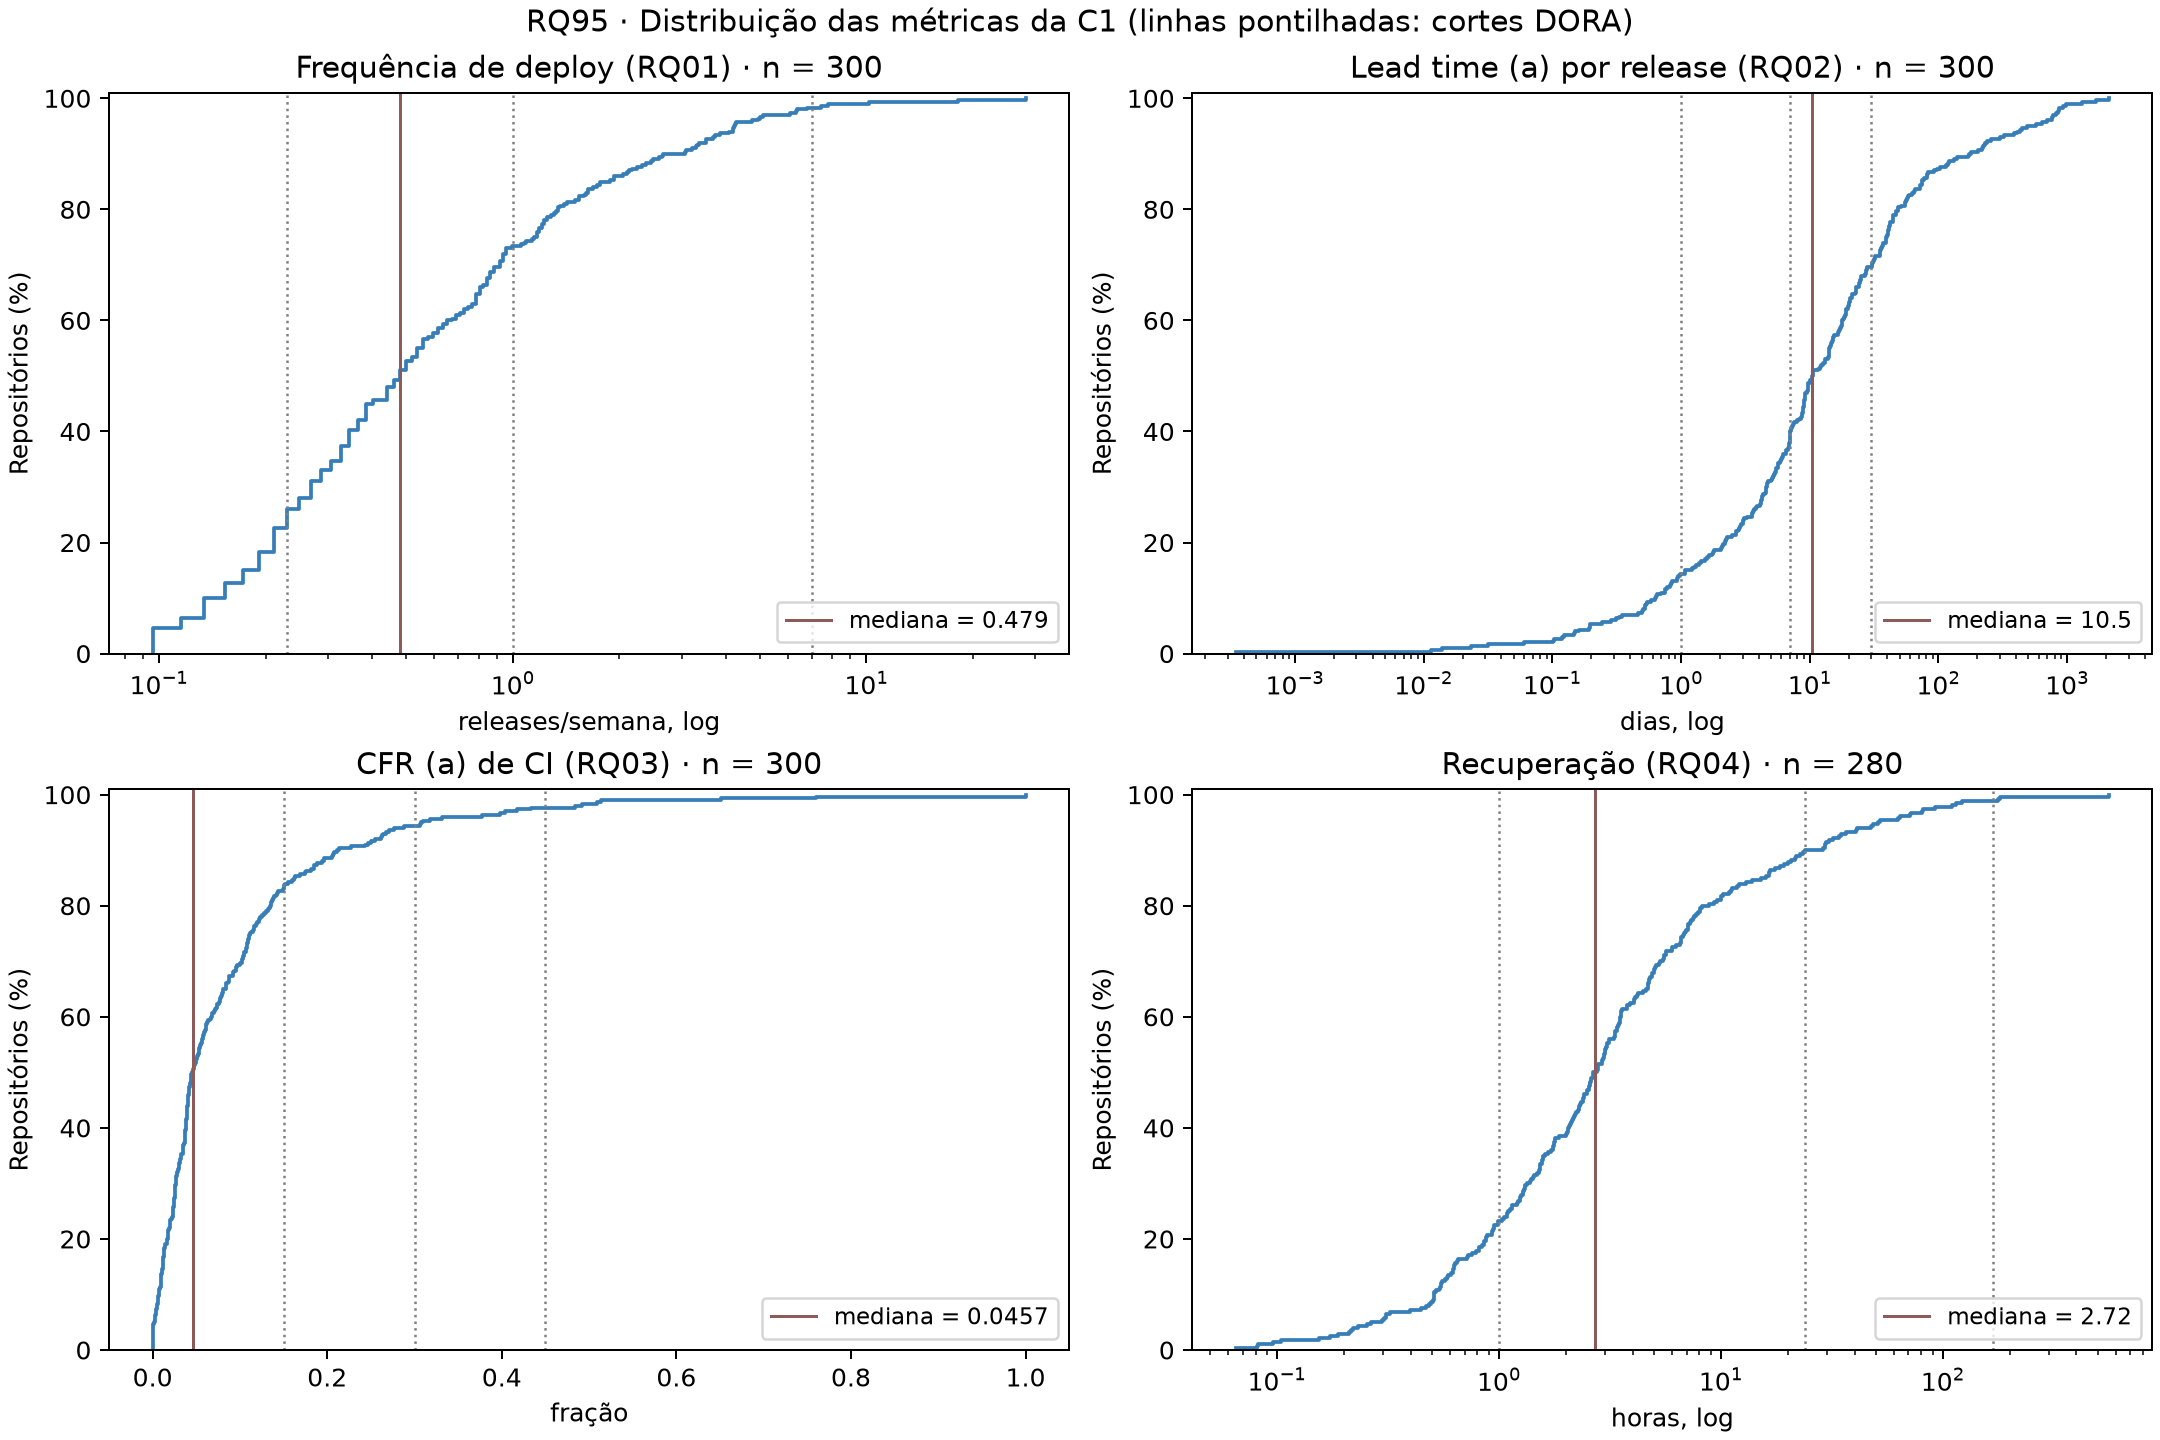
\includegraphics[width=0.92\linewidth]{figuras/distribuicoes_c1.png}
\caption{Distribuição acumulada das métricas da combinação C1 (linhas pontilhadas: cortes DORA;
linha vermelha: mediana).}
\label{fig:distribuicoes}
\end{figure}

\subsection{RQ01 --- Frequência de deploy}

A mediana é de 0,48 release/semana (IQR 0,93), com cauda longa à direita: o máximo é de 28,2
releases/semana e 33 repositórios passam do limite de Tukey (2,54). Os 30 repositórios mais
ativos (10\%) concentram 51,5\% das releases. Metade dos repositórios é Medium (50,7\%), um quarto é
High e só 5 (1,7\%) são Elite.

\subsection{RQ02 --- \textit{Lead time}}

Por release (a), a mediana é de 10,5 dias (IQR 35,9); por \textit{commit} (b), 12,1 dias (IQR 54,3).
Das 18.206 releases da janela, 14.589 têm \textit{lead time}; as demais são a primeira release
da história do repositório (57) ou não trazem \textit{commits} novos (3.560). A variante (b) é
menor que a (a) em 177 repositórios e maior em 122; a razão (b)/(a) tem mediana de 0,78 e o
teste de Wilcoxon pareado não rejeita a igualdade ($p = 0{,}12$). Trocar (a) por (b) muda a classe de
127 repositórios (42,3\%). Quanto maior a release, menor o (b) em relação ao (a)
($\rho = -0{,}30$ entre o número de \textit{commits} por release e a razão (b)/(a)).

\subsection{RQ03 --- Taxa de falha das mudanças}
\label{sec:rq03}

O CFR de CI (a) tem mediana de 4,6\% (IQR 8,8 pontos percentuais): 83,0\% dos repositórios são
Elite, e só 14 não têm nenhuma falha. O CFR de entrega (b), com a v1, tem mediana de 18,8\%
(IQR 44,7 pontos), muito mais disperso, e espalha os repositórios pelas quatro classes
(Tabela~\ref{tab:descritivo}). Somando todos os \textit{runs} e todas as releases, o CFR é de
9,2\% (a) e de 38,2\% (b). As duas variantes quase não concordam: $\rho = 0{,}07$ entre elas
($p = 0{,}26$), o (b) é maior que o (a) em 182 de 299 repositórios (Wilcoxon, $p < 10^{-15}$)
e 57,2\% dos repositórios mudam de classe ao trocar uma pela outra
($\kappa$ ponderado $= 0{,}02$, concordância leve), 144 deles para pior.

Os dois proxies medem coisas diferentes. No (a), 98,6\% das falhas são \texttt{failure} e 1,4\%
são \texttt{startup\_failure}, e o workflow que mais falha em cada repositório responde, na
mediana, por 73,1\% das falhas: o CFR (a) reflete sobretudo um ou dois \textit{workflows}. No
(b), 39,2\% das releases (7.130 de 18.206) têm tag fora do SemVer estrito e nunca são
corretivas na v1; 42 repositórios não têm nenhuma tag SemVer, e o CFR (b) deles é zero por
construção. Por outro lado, na mediana 42,9\% das releases de um repositório mudam só o
\textit{patch}. O nível do (b) depende da heurística: com as versões v2 (\textit{patch} ou qualquer
\textit{commit} com \texttt{fix}, \texttt{revert} ou \texttt{hotfix}) e v3 (correção de defeito),
a mediana vai a 43,5\% e 27,3\%, e 40,8\% e 31,8\% dos repositórios mudam de classe em relação à
v1. A v2 e a v3 marcam como corretivas 98,6\% e 61,3\% das releases na mediana, o que indica
excesso de marcações.

\begin{figure}[ht]
\centering
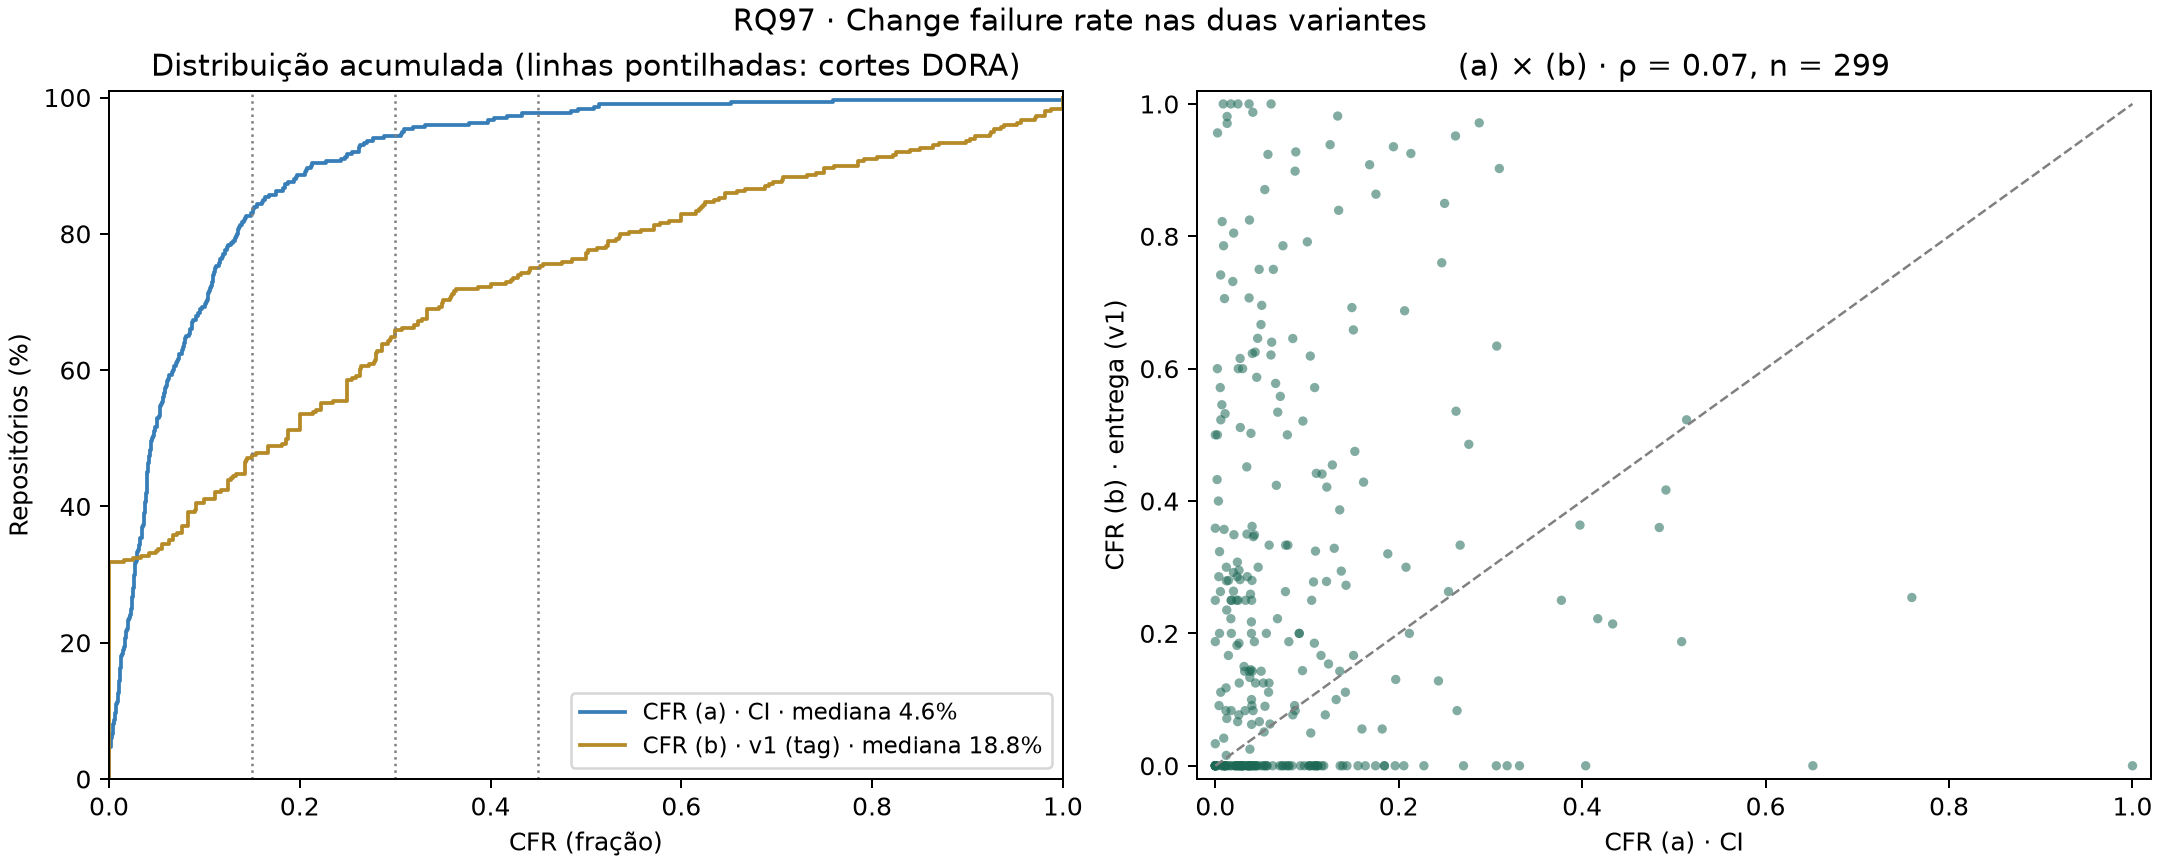
\includegraphics[width=0.95\linewidth]{figuras/cfr_variantes.png}
\caption{CFR nas duas variantes: distribuição acumulada (esquerda) e dispersão (a)~$\times$~(b)
(direita); linha tracejada: $y = x$.}
\label{fig:cfr}
\end{figure}

\subsection{RQ04 --- Tempo de recuperação}

Há 280 repositórios com tempo estimável (20 não têm nenhum episódio de falha completo e ficam
sem estimativa, não com zero). A mediana é de 2,7 horas (IQR 5,7), com cauda longa: o P90 é de
24,5 horas e o máximo, de 560 horas. Dos 27.839 episódios, 230 (0,83\%) terminam censurados à
direita, mas 24 repositórios têm pelo menos 10\% dos episódios censurados. Em 88,9\% dos
episódios a recuperação ocorre em até 24 horas (79,2\% com peso igual por repositório).

\subsection{Classificação DORA geral}

Pela combinação de referência C1 (release, \textit{lead time} (a), CFR (a)), 280 repositórios
recebem classe geral: 6,4\% Elite, 43,6\% High, 45,7\% Medium e 4,3\% Low; os 20 repositórios sem
episódio de falha completo ficam sem classe. A estabilidade é alta (Elite ou High nas duas métricas
da dimensão) em 85,4\% dos repositórios classificados, mas só 21,1\% têm velocidade alta. A classe
geral é limitada pela velocidade, não pela estabilidade.

\subsection{RQ05 --- Frequência de deploy e CFR}
\label{sec:rq05}

\begin{table}[ht]
\centering
\small
\caption{Correlação de Spearman entre a frequência de deploy e o CFR (IC de 95\% por
\textit{bootstrap}; $p$ com correção de Holm). O $\rho$ parcial controla idade e contribuidores
no (a) e o CFR (b) esperado ao acaso no (b) (Seção~\ref{sec:discussao}).}
\label{tab:rq05}
\begin{tabular}{lrrrrr}
\hline
Variante & $n$ & $\rho$ & $p$ (Holm) & IC 95\% & $\rho$ parcial \\
\hline
CFR (a), CI           & 300 & 0,15 & 0,009            & 0,04 a 0,27 & 0,09 ($p = 0{,}14$) \\
CFR (b), entrega (v1) & 299 & 0,40 & $2 \times 10^{-12}$ & 0,29 a 0,51 & $-0{,}16$ ($p = 0{,}005$) \\
\hline
\end{tabular}
\end{table}

A frequência de deploy tem correlação fraca e positiva com o CFR (a) e moderada e positiva com o CFR (b)
(Tabela~\ref{tab:rq05}, Figura~\ref{fig:rq05}). Em quartis de frequência, a mediana do CFR (a) fica
em torno de 4--7\% em todas as faixas, enquanto a do CFR (b) sobe de 0\% (Q1) para 44,2\% (Q4).
Em termos de classes, 94\% dos repositórios de frequência alta (Elite ou High) têm CFR (a) Elite
ou High, contra 95\% dos de frequência baixa (Fisher, $p = 0{,}78$); no CFR (b), 40\% contra 75\%
($p < 10^{-7}$).

\begin{figure}[ht]
\centering
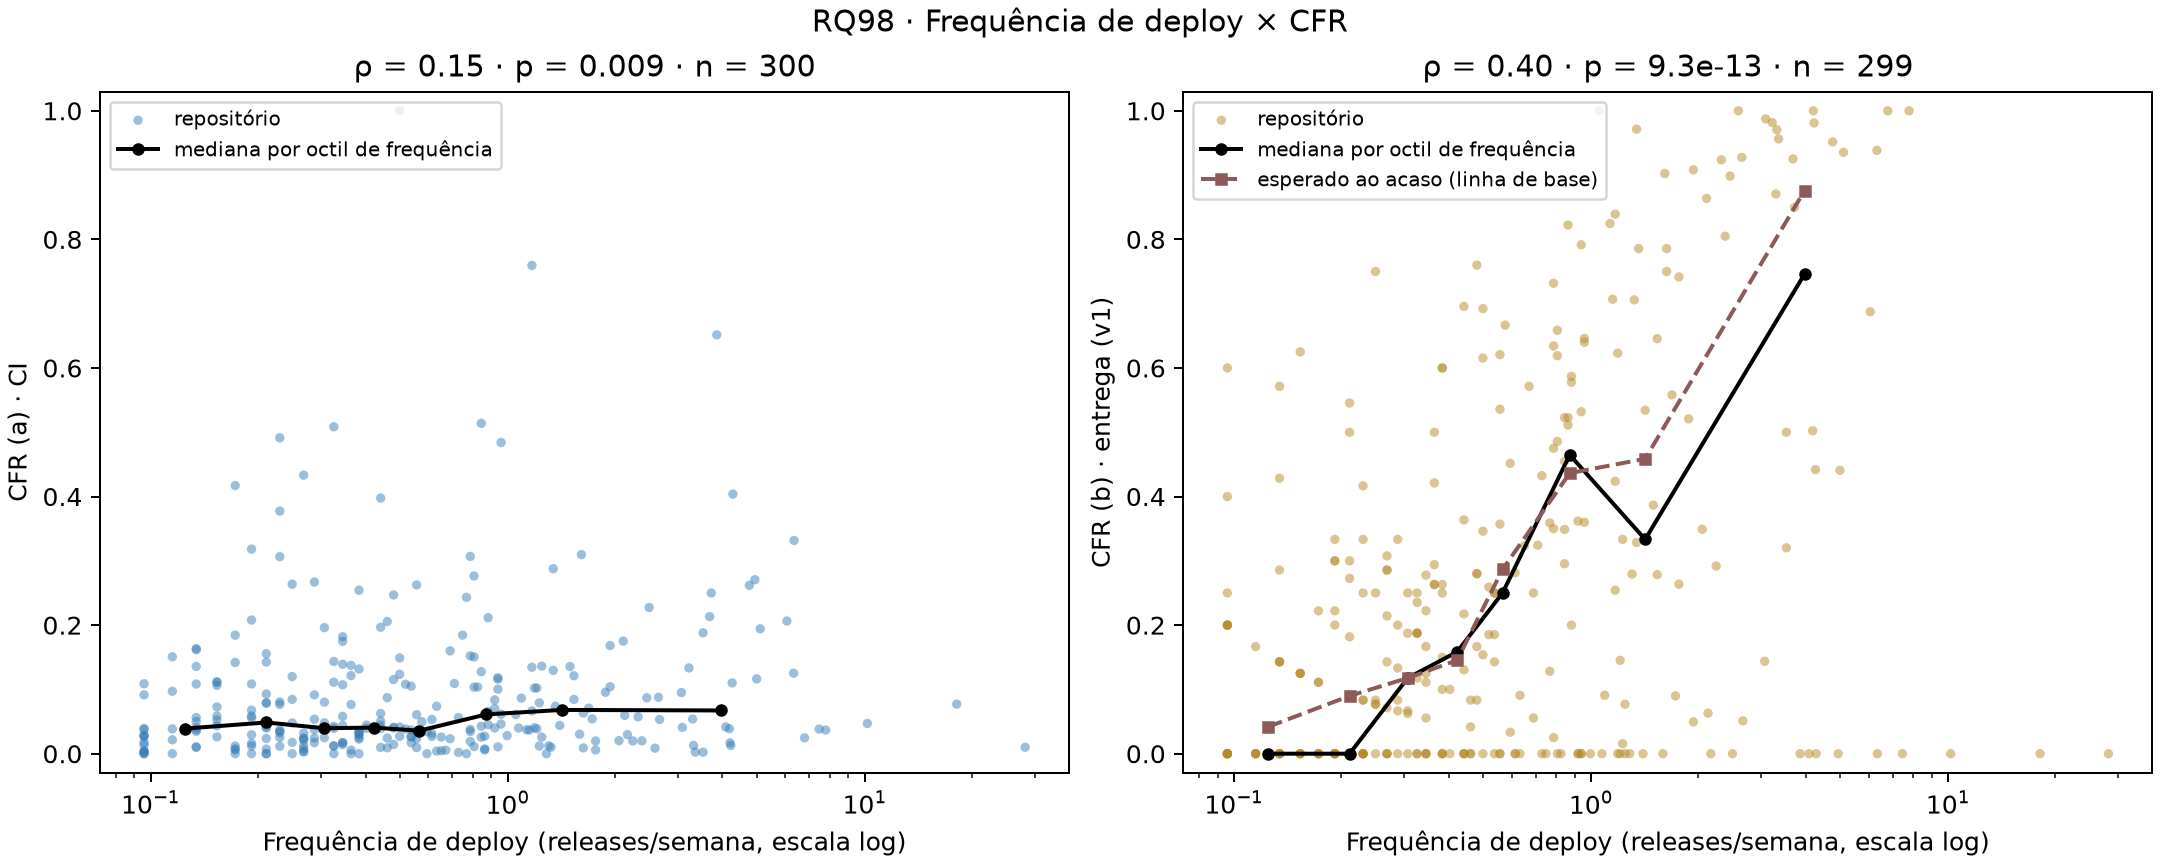
\includegraphics[width=0.95\linewidth]{figuras/dispersao_df_cfr.png}
\caption{Frequência de deploy (escala logarítmica) e CFR. Linha preta: mediana por octil de
frequência; linha tracejada: CFR (b) esperado ao acaso (linha de base da Seção~\ref{sec:discussao}).}
\label{fig:rq05}
\end{figure}

\subsection{RQ06 --- Características dos repositórios}
\label{sec:rq06}

\apreencher{resultados da RQ06 (issue \#93): Kruskal-Wallis ou Mann-Whitney por fator, p-valores
com correção de Holm, $\varepsilon^2$ e $\delta$ de Cliff}

\subsection{RQ07 --- Sensibilidade da classificação DORA}

Classificamos cada repositório em sete combinações de definições (C1 a C7, Tabela~\ref{tab:rq07}).
Dos 279 repositórios classificados em todas elas, 163 (58,4\%) têm a mesma classe geral em todas
e 116 (41,6\%) mudam em pelo menos uma alternativa à C1. Trocar só a unidade de deploy (C5 e C6)
muda de 3,6\% a 10,7\% das classes, sempre para melhor ($\kappa$ de 0,85 a 0,95); as
combinações com o CFR (b) mudam de 20,8\% a 35,5\%, e 75\% das mudanças são para pior. No nível
de cada métrica, trocar o CFR (a) pelo (b) muda a classe de 57,2\% dos repositórios
($\kappa = 0{,}02$), o \textit{lead time} (a) pelo (b), de 42,3\%, e a unidade de deploy de
release para tag, de 24,0\%.

\begin{table}[ht]
\centering
\small
\caption{Mudança da classe geral em relação à C1 (279 a 280 repositórios por par).}
\label{tab:rq07}
\begin{tabular}{llrrl}
\hline
Combinação & O que muda em relação à C1 & Mudam (\%) & $\kappa$ pond. & Landis--Koch \\
\hline
C2 & \textit{lead time} (b)                     & 14,3 & 0,79 & substancial \\
C3 & CFR (b)                                    & 20,8 & 0,68 & substancial \\
C4 & \textit{lead time} (b) e CFR (b)           & 29,7 & 0,52 & moderada \\
C5 & pré-releases contam como deploy            & 3,6  & 0,95 & quase perfeita \\
C6 & tags contam como deploy                    & 10,7 & 0,85 & quase perfeita \\
C7 & tags, \textit{lead time} (b) e CFR (b)     & 35,5 & 0,44 & moderada \\
\hline
\end{tabular}
\end{table}
 depois de % Secao 2 do artigo do LAB03 (template SBC). Issue #90.
% Uso no Overleaf: \input{metodologia} depois de \input{introducao}.
% Requer os mesmos pacotes da introducao (nada alem do template).
%
% Trechos entre \apreencher{...} dependem de dados que ainda nao existem (amostra
% final de 300, rotulos humanos, consenso, F1) ou de confirmacao do professor
% (janela oficial). Nao ha numero inventado: o funil e o piloto da Sprint 01 sao
% identificados como tais. Busque por "apreencher" antes de entregar.

\providecommand{\apreencher}[1]{\textbf{[a preencher: #1]}}

\section{Metodologia}
\label{sec:metodologia}

\subsection{Visão geral}

O estudo calcula as quatro métricas DORA, a partir de dados públicos do GitHub,
para repositórios \textit{open-source} populares que usam GitHub Actions, e mede
a confiabilidade dessas medidas por duas vias: a validação manual das
heurísticas (Seção~\ref{sec:validacao}) e a análise de sensibilidade às
definições operacionais (RQ07). Todas as definições abaixo são comuns à turma,
para que os resultados sejam comparáveis e o pipeline possa ser replicado por
outro grupo (Seção~6).

\subsection{Fonte de dados e coleta}
\label{sec:coleta}

A coleta usa um cliente próprio das APIs REST e GraphQL do GitHub, sem
bibliotecas de acesso à API. A busca de candidatos (\texttt{GET
/search/repositories}) é fatiada por faixas de estrelas para contornar o teto de
1.000 resultados por consulta, e reúne 8.000 candidatos. Os metadados de cada
um (estrelas, linguagem principal, data de criação, \textit{default branch},
indicadores de \textit{fork}, arquivamento e repositório vazio) vêm da API
GraphQL. Para os repositórios aceitos, o pipeline coleta, pela API REST, as
releases (\texttt{/releases}), os \textit{commits} entre releases consecutivas
(\texttt{/compare}, com paginação para ultrapassar o limite de 250 \textit{commits}),
as tags e as execuções de \textit{workflow} (\texttt{/actions/runs}) do
\textit{default branch}.

Duas decisões de coleta afetam a validade. Primeiro, a busca de execuções
retorna no máximo 1.000 resultados por consulta; por isso a janela é consultada
mês a mês e qualquer intervalo que atinja o teto é dividido ao meio (até o
nível de segundos), de modo que nenhuma execução se perde sem aviso. Segundo, o
pipeline descarta repositórios com mais de 20.000 execuções na janela, por custo
de coleta; esse limite é contabilizado no funil e discutido como limitação.

A coleta é um pipeline reprodutível, executado por um único comando. Toda
resposta da API é gravada em disco (um arquivo por URL), o que permite retomar
uma coleta interrompida sem repetir chamadas. O cliente lê os cabeçalhos
\texttt{X-RateLimit-Remaining} e \texttt{X-RateLimit-Reset} e espera
sozinho quando a cota acaba. Erros temporários (respostas 5xx e quedas de rede)
são repetidos com \textit{backoff} exponencial (1~s, 2~s, 4~s, \ldots, até 60~s,
em até 6 tentativas). O \textit{token} vem de variável de ambiente e nunca é
versionado. As funções que calculam as métricas têm testes automatizados
(\textit{pytest}, cobertura mínima de 80\% do módulo de métricas, medida com
\textit{pytest-cov}) executados no GitHub Actions do grupo a cada \textit{push}.

\subsection{Seleção da amostra e funil}
\label{sec:funil}

Os candidatos são avaliados em ordem decrescente de estrelas, do critério mais
barato ao mais caro, até se atingir a meta de pelo menos 300 repositórios. Um
repositório entra na amostra se (i) não é \textit{fork}, está ativo (não
arquivado, desabilitado ou vazio) e tem \textit{default branch}; (ii) usa GitHub
Actions (\texttt{total\_count > 0} em \texttt{/actions/workflows}); (iii) tem
pelo menos 5 releases publicadas na janela; e (iv) tem pelo menos 50 execuções
válidas no \textit{default branch} na janela. Os critérios não são relaxados para
atingir a meta. A Tabela~\ref{tab:funil} mostra o funil; as colunas trazem o
piloto da primeira sprint (meta de 100) e a amostra final.

\begin{table}[ht]
\centering
\small
\caption{Funil de seleção. O piloto (Sprint 01) foi coletado com a janela
provisória; a amostra final ainda não foi exportada.}
\label{tab:funil}
\begin{tabular}{lrr}
\hline
Etapa & Piloto ($n=100$) & Final \\
\hline
Candidatos com metadados & 8.000 & \apreencher{n} \\
Ativos (sem \textit{fork}/arquivados/vazios) & 7.519 & \apreencher{n} \\
Avaliados até a meta & 272 & \apreencher{n} \\
Usam GitHub Actions & 253 & \apreencher{n} \\
$\geq 5$ releases na janela & 132 & \apreencher{n} \\
$\leq 20.000$ execuções (custo) & 114 & \apreencher{n} \\
$\geq 50$ execuções válidas & 100 & \apreencher{$\geq 300$} \\
\hline
\end{tabular}
\end{table}

\subsection{Definições operacionais}
\label{sec:definicoes}

\begin{table}[ht]
\centering
\small
\caption{Definições operacionais comuns à turma.}
\label{tab:definicoes}
\begin{tabular}{p{0.22\linewidth}p{0.68\linewidth}}
\hline
Elemento & Definição \\
\hline
Janela & 12 meses, de 01/10/2025 a 30/09/2026, com as duas datas inclusivas
\apreencher{confirmar a janela oficial com o professor} \\
\textit{Branch} & Apenas o \textit{default branch} (\texttt{default\_branch}) \\
Deploy & Release publicada (\texttt{draft = false}) e não pré-release;
pré-releases e tags são variantes da RQ07 \\
Data do \textit{commit} & \texttt{commit.author.date} \\
Execução de CI & \textit{Workflow run} do \textit{default branch} com
\texttt{event = push}, criado na janela \\
Sucesso & \texttt{success} \\
Falha & \texttt{failure}, \texttt{timed\_out}, \texttt{startup\_failure} \\
Ignorada & \texttt{cancelled}, \texttt{skipped}, \texttt{neutral},
\texttt{action\_required}, \texttt{stale} ou vazio \\
Censura & Evento final não observado na janela: registrado como censurado, não
descartado \\
\hline
\end{tabular}
\end{table}

\subsection{Métricas e variantes}
\label{sec:metricas}

Em todas as RQs reportamos mediana e intervalo interquartil (IQR, quartis por
interpolação linear), e não média e desvio-padrão, porque as distribuições são
assimétricas.

\textbf{RQ01 -- Frequência de deploy.} Releases publicadas na janela divididas
pelo número de semanas da janela ($\approx 52{,}1$).

\textbf{RQ02 -- \textit{Lead time}.} Para cada release R da janela, os
\textit{commits} são os do \texttt{compare} com a release publicada
imediatamente anterior, que pode estar fora da janela. Na variante (a), o
\textit{lead time} de R é a data de R menos a do \textit{commit} mais antigo, e o
valor do repositório é a mediana entre as releases. Na variante (b), cada
\textit{commit} contribui com a data de R menos a sua, e o valor do repositório é
a mediana de todos os \textit{commits} de todas as releases (e não uma mediana de
medianas). Decisões do grupo: a primeira release da história do repositório é
ignorada; \texttt{compare} indisponível (por exemplo, tag apagada) ou truncado
exclui a release do cálculo e é contado; uma release sem \textit{commits} novos
fica fora das duas variantes; e um \textit{commit} com data de autoria posterior
à da release (relógio errado ou tag movida) é descartado e contado.

\textbf{RQ03 -- Taxa de falha (CFR).} A variante (a), de CI, é o número de
execuções com falha dividido por falhas mais sucessos, considerando todos os
\textit{workflows} juntos; ela mede falha de pipeline, não de produção. A
variante (b), de entrega, considera uma release R como falha se for seguida, em
até 7 dias (inclusive), por uma release corretiva; o CFR é o número de releases
que falharam dividido pelo de avaliadas. Várias corretivas na semana não
multiplicam a falha de R. Releases dos últimos 7 dias da janela são censuradas e
ficam fora do denominador.

\textbf{RQ04 -- Tempo de recuperação.} Dentro de cada \textit{workflow}, um
episódio de falha começa na primeira falha após um sucesso e termina no próximo
sucesso; sua duração é o \texttt{updated\_at} do sucesso menos o
\texttt{run\_started\_at} da falha. Execuções ignoradas não interrompem nem
iniciam episódios. O valor do repositório é a mediana dos episódios de todos os
seus \textit{workflows}. Episódios sem sucesso até o fim da janela são
censurados à direita. Por decisão do grupo, também são censurados (à esquerda)
os episódios de um \textit{workflow} cuja primeira execução válida na janela já
é uma falha, pois o início real é desconhecido. Episódios censurados não entram
na mediana, e a proporção deles é reportada por repositório. Repositório sem
falhas tem recuperação indefinida (e não zero).

\textbf{Classificação DORA.} Cada métrica recebe 4 (Elite), 3 (High), 2 (Medium)
ou 1 (Low) pelos cortes fixos da disciplina; a categoria geral é a mediana dos
quatro valores, arredondada para baixo.

\subsection{Heurística de release corretiva}
\label{sec:heuristica}

Uma release é corretiva quando seu objetivo principal é corrigir um defeito
recente. Como o GitHub não registra isso, usamos heurísticas sobre a tag e sobre
a primeira linha das mensagens dos \textit{commits} entre a release anterior e a
avaliada. Testamos três versões, aplicadas sempre em relação à release publicada
imediatamente anterior:

\begin{itemize}
  \item \textbf{v1 (\textit{patch} SemVer):} só o número de \textit{patch}
  mudou (por exemplo, $2.3.0 \rightarrow 2.3.1$). Tags que não seguem SemVer
  estrito, pré-releases e \textit{downgrades} nunca são corretivas.
  \item \textbf{v2 (\textit{patch} ou mensagem):} v1, ou algum \textit{commit}
  com \texttt{revert}, \texttt{hotfix} ou \texttt{fix}.
  \item \textbf{v3 (correção de defeito):} \texttt{revert} ou \texttt{hotfix}
  bastam; caso contrário, exige \textit{commit} \texttt{fix} que não trate de
  \textit{typo}, documentação, CI, testes ou dependências, e que o \textit{patch}
  tenha mudado ou que ao menos metade dos \textit{commits} (sem \textit{merges}) seja
  correção, sem \textit{commit} de funcionalidade. Sem mensagens disponíveis,
  vale só a tag.
\end{itemize}

A versão usada no CFR (b) é a que atingir F1~$\geq 0{,}70$ contra o consenso
da amostra-ouro; se nenhuma atingir, a heurística é refinada e reavaliada, e
todas as versões e seus F1 são reportadas. Resultados:
\apreencher{P, R e F1 de v1, v2, v3 e das versões seguintes}.
As heurísticas não leem as \textit{release notes} nem o \textit{diff}; isso é
uma limitação.

\subsection{Validação manual (amostra-ouro)}
\label{sec:validacao}

Sorteamos 60 repositórios da amostra final com \texttt{df.sample(n=60,
random\_state=42)}, sobre a amostra ordenada por nome (a ordem do arquivo não
altera o sorteio), e, em cada um, até 5 releases da definição principal de
deploy que tenham release anterior (a primeira da história fica de fora, pois
não há lista de \textit{commits} para ler). Os três integrantes rotularam, de
forma independente, sem consultar os demais e sem ver a saída da heurística, em
planilhas idênticas com ligações para a página da release e para o
\texttt{compare}: (i)~o tipo do projeto (biblioteca/\textit{framework},
aplicação/serviço, ferramenta CLI ou outro); (ii)~se as releases representam
entregas reais ao usuário (sim, não ou incerto); e (iii)~se cada release
sorteada é corretiva (sim ou não).

A concordância entre os três avaliadores é medida com o $\kappa$ de Fleiss em
cada dimensão (interpretação de Landis e Koch). Os casos divergentes são
discutidos pelo grupo e geram o rótulo de consenso; o protocolo de desempate é
\apreencher{protocolo definido na consolidação do consenso}. Um $\kappa$ baixo é
tratado como achado sobre a ambiguidade do critério. A heurística é avaliada
contra o consenso com precisão, \textit{recall} e F1 (classe positiva:
corretiva). Como as regras são ajustadas olhando os erros desta mesma amostra, o
F1 final tende a ser otimista. Resultados: \apreencher{$\kappa$ por dimensão,
tamanho do consenso}. O tipo do projeto rotulado alimenta a RQ06.

\subsection{Análise estatística}
\label{sec:analise}

Para a RQ05, usamos a correlação de Spearman ($\rho$, p-valor e $n$) entre a
frequência de deploy e o CFR, separadamente para as variantes (a) e (b). Na RQ06,
comparamos as métricas entre subgrupos de pelo menos três fatores (linguagem,
quartis de estrelas, de contribuidores e de idade, e tipo do projeto) com
Kruskal-Wallis (ou Mann-Whitney, quando há dois grupos), corrigimos os p-valores
por Holm e reportamos o tamanho de efeito ($\varepsilon^2 = H/(n-1)$ ou
$\delta$ de Cliff). Na RQ07, montamos ao menos três combinações de definições
(por exemplo, release, release com pré-release e tag como unidade de deploy,
combinadas com as variantes de \textit{lead time} e de CFR), classificamos cada
repositório em cada combinação e calculamos, por par, a proporção que muda de
categoria e o $\kappa$ de Cohen ponderado (pesos lineares).

\subsection{Disponibilidade}

O código, os testes, o dicionário de dados e os CSVs finais estão no
repositório do grupo (Seção~7). O pipeline é executável por outro grupo com um
único comando, conforme o README.
; as figuras ficam em figuras/
% (\usepackage{graphicx}, ja no template).
%
% Todos os numeros vem das analises do repositorio (entregas/laboratorio-03/sprint-03):
% RQ91 (RQ01), RQ94 (RQ02), RQ97 (RQ03), RQ92 (RQ04), RQ95 (classificacao C1),
% RQ98 (RQ05), RQ96 (RQ07). Janela provisoria; CFR (b) com a heuristica v1, ainda sem F1 medido.
% Trechos em \apreencher{...} dependem de analises ainda nao feitas (RQ06, issue #93) ou da
% validacao manual (issues #85 a #89). Busque por "apreencher" antes de entregar.

\providecommand{\apreencher}[1]{\textbf{[a preencher: #1]}}

\section{Resultados}
\label{sec:resultados}

Os resultados se referem aos 300 repositórios da amostra final (Seção~\ref{sec:funil}),
na janela de 01/10/2025 a 30/09/2026, ainda provisória (Seção~\ref{sec:definicoes}). Cada
repositório tem o mesmo peso e a estatística da amostra é a mediana dos valores dos
repositórios, com o intervalo interquartil (IQR, Q1--Q3). A Tabela~\ref{tab:descritivo} resume
as métricas e a classificação DORA de cada uma. Nas Seções~\ref{sec:rq03} e~\ref{sec:rq05},
o CFR (b) usa a versão v1 da heurística de release corretiva, que ainda não tem F1 medido
contra o consenso da amostra-ouro (\apreencher{P, R e F1 das versões v1, v2 e v3}).

\begin{table}[ht]
\centering
\small
\caption{Métricas DORA e classes (\% dos repositórios com a métrica definida). Frequência em
releases/semana; \textit{lead time} em dias; CFR em \%; recuperação em horas.}
\label{tab:descritivo}
\begin{tabular}{lrrrrrr}
\hline
Métrica & $n$ & Mediana (Q1--Q3) & Elite & High & Medium & Low \\
\hline
Frequência de deploy      & 300 & 0,48 (0,23--1,16) & 1,7  & 25,0 & 50,7 & 22,7 \\
\textit{Lead time} (a)    & 300 & 10,5 (3,6--39,5)  & 14,3 & 25,0 & 30,3 & 30,3 \\
\textit{Lead time} (b)    & 300 & 12,1 (3,3--57,5)  & 10,3 & 28,7 & 28,7 & 32,3 \\
CFR (a), CI               & 300 & 4,6 (2,3--11,1)   & 83,0 & 11,3 & 3,3  & 2,3  \\
CFR (b), entrega (v1)     & 299 & 18,8 (0,0--44,7)  & 47,5 & 18,4 & 9,0  & 25,1 \\
Recuperação               & 280 & 2,7 (1,1--6,9)    & 23,2 & 66,4 & 9,3  & 1,1  \\
\hline
Classe geral (C1)         & 280 & ---               & 6,4  & 43,6 & 45,7 & 4,3  \\
\hline
\end{tabular}
\end{table}

\begin{figure}[ht]
\centering
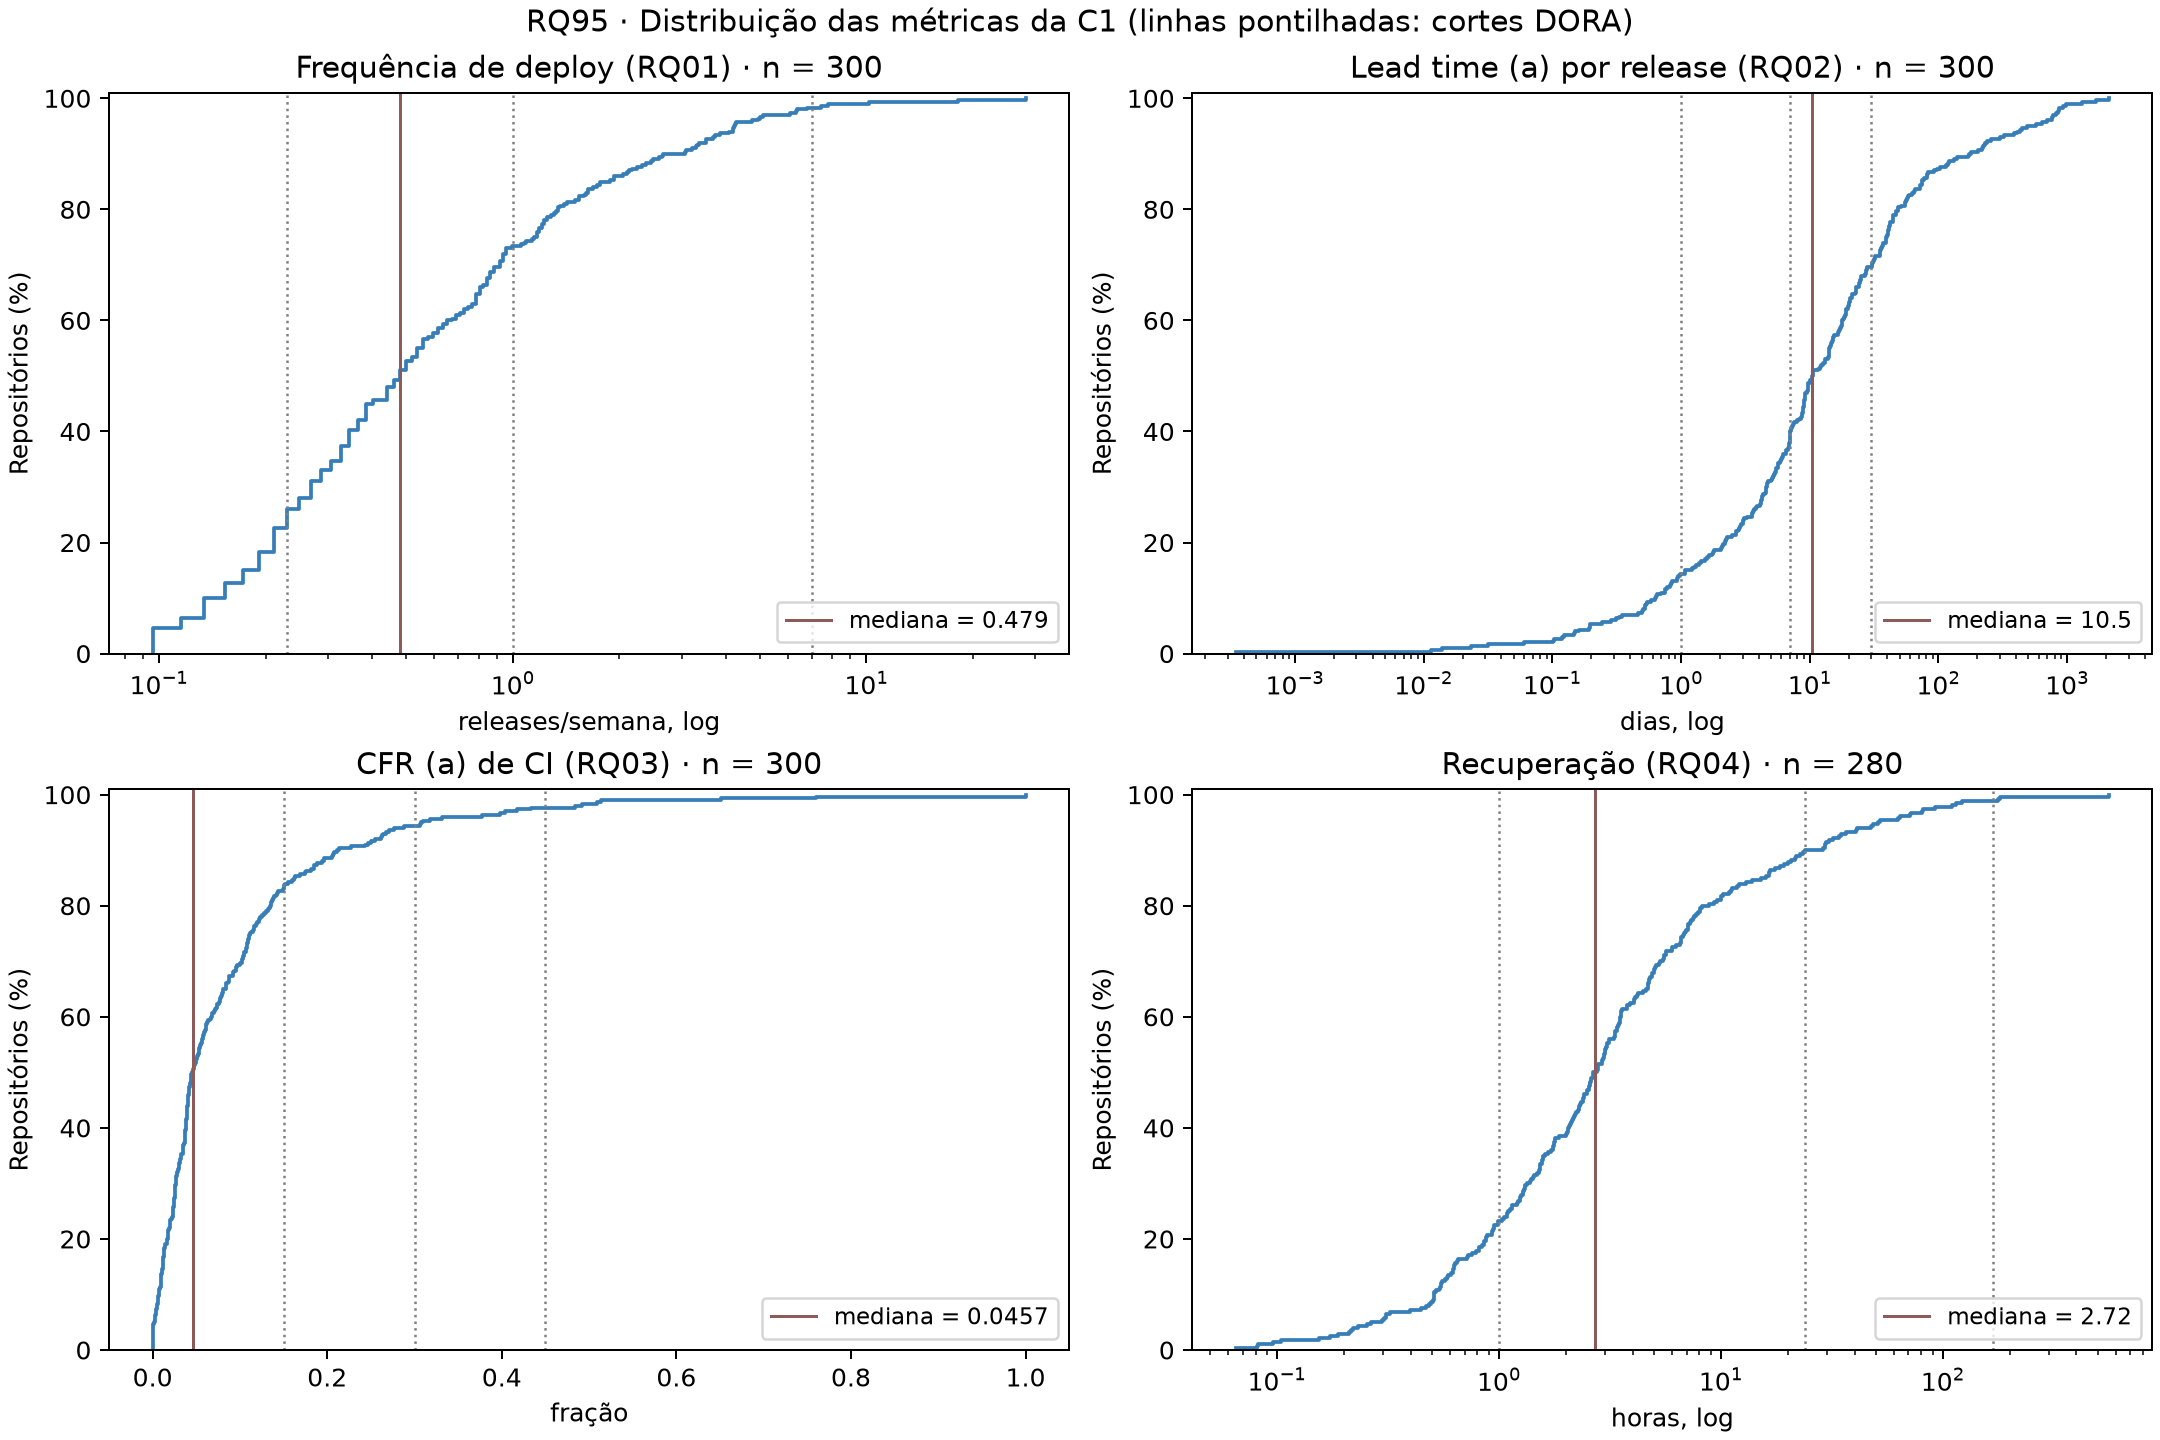
\includegraphics[width=0.92\linewidth]{figuras/distribuicoes_c1.png}
\caption{Distribuição acumulada das métricas da combinação C1 (linhas pontilhadas: cortes DORA;
linha vermelha: mediana).}
\label{fig:distribuicoes}
\end{figure}

\subsection{RQ01 --- Frequência de deploy}

A mediana é de 0,48 release/semana (IQR 0,93), com cauda longa à direita: o máximo é de 28,2
releases/semana e 33 repositórios passam do limite de Tukey (2,54). Os 30 repositórios mais
ativos (10\%) concentram 51,5\% das releases. Metade dos repositórios é Medium (50,7\%), um quarto é
High e só 5 (1,7\%) são Elite.

\subsection{RQ02 --- \textit{Lead time}}

Por release (a), a mediana é de 10,5 dias (IQR 35,9); por \textit{commit} (b), 12,1 dias (IQR 54,3).
Das 18.206 releases da janela, 14.589 têm \textit{lead time}; as demais são a primeira release
da história do repositório (57) ou não trazem \textit{commits} novos (3.560). A variante (b) é
menor que a (a) em 177 repositórios e maior em 122; a razão (b)/(a) tem mediana de 0,78 e o
teste de Wilcoxon pareado não rejeita a igualdade ($p = 0{,}12$). Trocar (a) por (b) muda a classe de
127 repositórios (42,3\%). Quanto maior a release, menor o (b) em relação ao (a)
($\rho = -0{,}30$ entre o número de \textit{commits} por release e a razão (b)/(a)).

\subsection{RQ03 --- Taxa de falha das mudanças}
\label{sec:rq03}

O CFR de CI (a) tem mediana de 4,6\% (IQR 8,8 pontos percentuais): 83,0\% dos repositórios são
Elite, e só 14 não têm nenhuma falha. O CFR de entrega (b), com a v1, tem mediana de 18,8\%
(IQR 44,7 pontos), muito mais disperso, e espalha os repositórios pelas quatro classes
(Tabela~\ref{tab:descritivo}). Somando todos os \textit{runs} e todas as releases, o CFR é de
9,2\% (a) e de 38,2\% (b). As duas variantes quase não concordam: $\rho = 0{,}07$ entre elas
($p = 0{,}26$), o (b) é maior que o (a) em 182 de 299 repositórios (Wilcoxon, $p < 10^{-15}$)
e 57,2\% dos repositórios mudam de classe ao trocar uma pela outra
($\kappa$ ponderado $= 0{,}02$, concordância leve), 144 deles para pior.

Os dois proxies medem coisas diferentes. No (a), 98,6\% das falhas são \texttt{failure} e 1,4\%
são \texttt{startup\_failure}, e o workflow que mais falha em cada repositório responde, na
mediana, por 73,1\% das falhas: o CFR (a) reflete sobretudo um ou dois \textit{workflows}. No
(b), 39,2\% das releases (7.130 de 18.206) têm tag fora do SemVer estrito e nunca são
corretivas na v1; 42 repositórios não têm nenhuma tag SemVer, e o CFR (b) deles é zero por
construção. Por outro lado, na mediana 42,9\% das releases de um repositório mudam só o
\textit{patch}. O nível do (b) depende da heurística: com as versões v2 (\textit{patch} ou qualquer
\textit{commit} com \texttt{fix}, \texttt{revert} ou \texttt{hotfix}) e v3 (correção de defeito),
a mediana vai a 43,5\% e 27,3\%, e 40,8\% e 31,8\% dos repositórios mudam de classe em relação à
v1. A v2 e a v3 marcam como corretivas 98,6\% e 61,3\% das releases na mediana, o que indica
excesso de marcações.

\begin{figure}[ht]
\centering
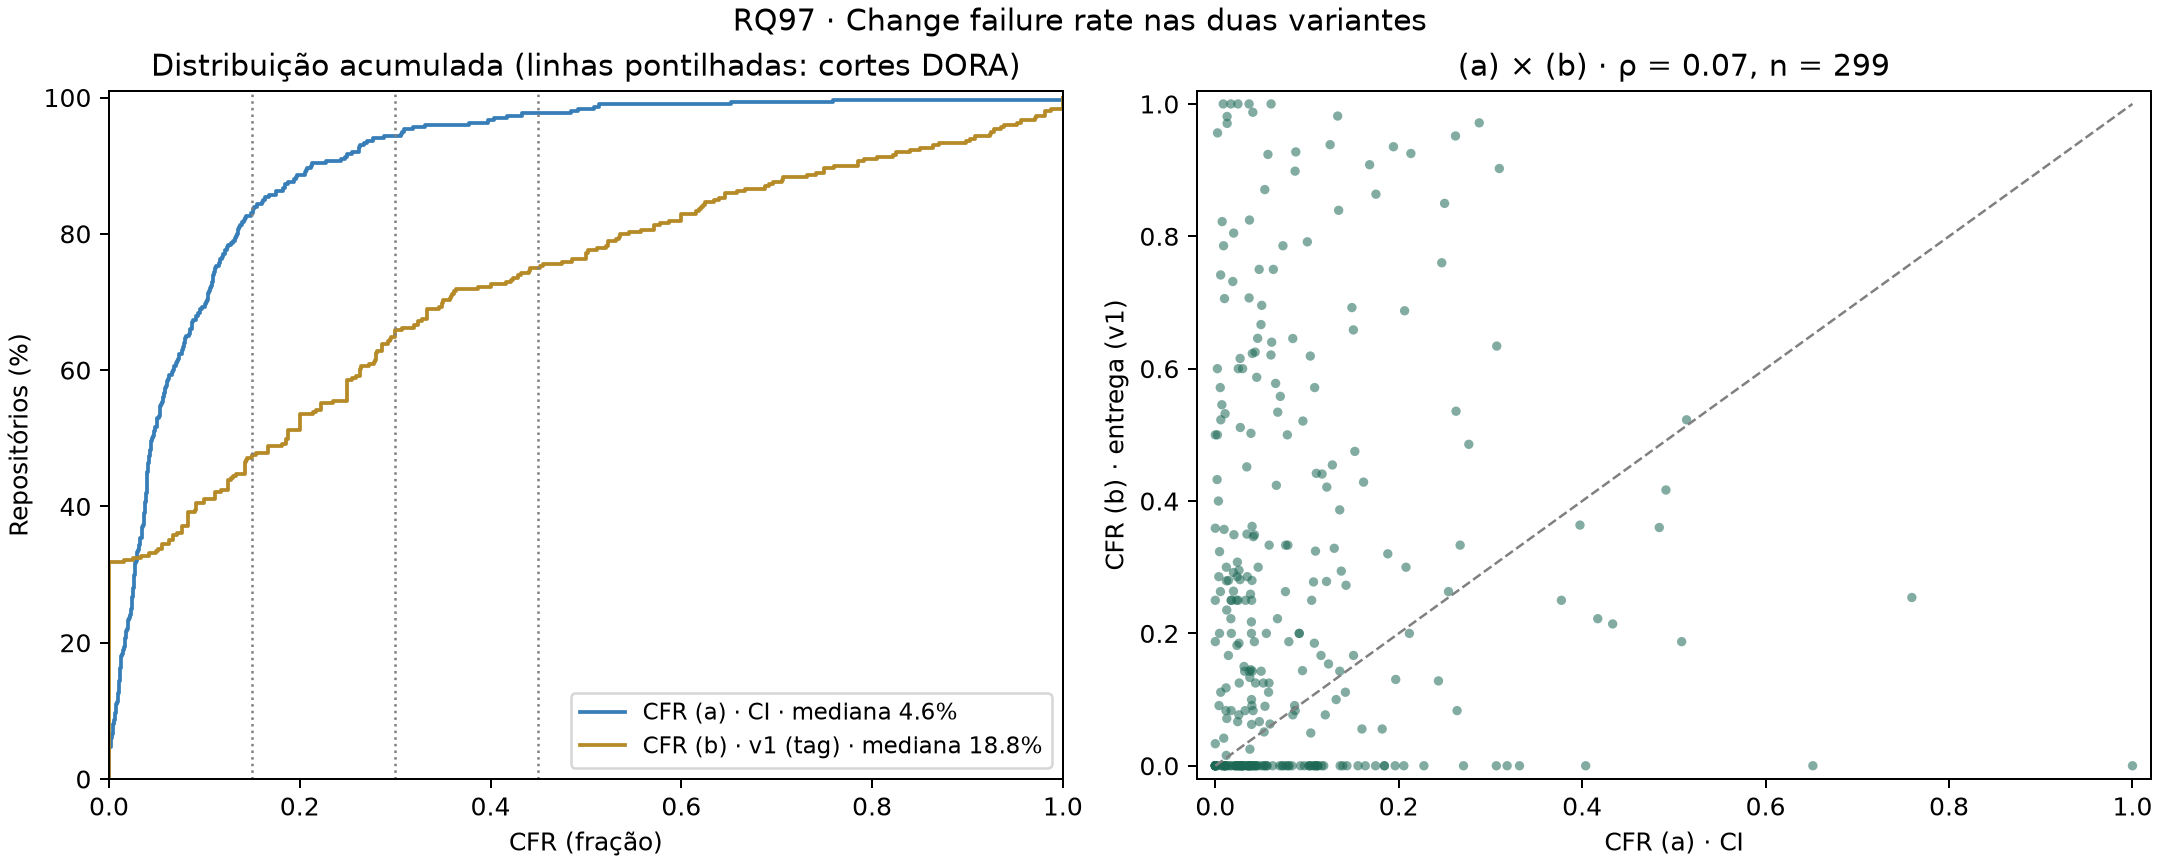
\includegraphics[width=0.95\linewidth]{figuras/cfr_variantes.png}
\caption{CFR nas duas variantes: distribuição acumulada (esquerda) e dispersão (a)~$\times$~(b)
(direita); linha tracejada: $y = x$.}
\label{fig:cfr}
\end{figure}

\subsection{RQ04 --- Tempo de recuperação}

Há 280 repositórios com tempo estimável (20 não têm nenhum episódio de falha completo e ficam
sem estimativa, não com zero). A mediana é de 2,7 horas (IQR 5,7), com cauda longa: o P90 é de
24,5 horas e o máximo, de 560 horas. Dos 27.839 episódios, 230 (0,83\%) terminam censurados à
direita, mas 24 repositórios têm pelo menos 10\% dos episódios censurados. Em 88,9\% dos
episódios a recuperação ocorre em até 24 horas (79,2\% com peso igual por repositório).

\subsection{Classificação DORA geral}

Pela combinação de referência C1 (release, \textit{lead time} (a), CFR (a)), 280 repositórios
recebem classe geral: 6,4\% Elite, 43,6\% High, 45,7\% Medium e 4,3\% Low; os 20 repositórios sem
episódio de falha completo ficam sem classe. A estabilidade é alta (Elite ou High nas duas métricas
da dimensão) em 85,4\% dos repositórios classificados, mas só 21,1\% têm velocidade alta. A classe
geral é limitada pela velocidade, não pela estabilidade.

\subsection{RQ05 --- Frequência de deploy e CFR}
\label{sec:rq05}

\begin{table}[ht]
\centering
\small
\caption{Correlação de Spearman entre a frequência de deploy e o CFR (IC de 95\% por
\textit{bootstrap}; $p$ com correção de Holm). O $\rho$ parcial controla idade e contribuidores
no (a) e o CFR (b) esperado ao acaso no (b) (Seção~\ref{sec:discussao}).}
\label{tab:rq05}
\begin{tabular}{lrrrrr}
\hline
Variante & $n$ & $\rho$ & $p$ (Holm) & IC 95\% & $\rho$ parcial \\
\hline
CFR (a), CI           & 300 & 0,15 & 0,009            & 0,04 a 0,27 & 0,09 ($p = 0{,}14$) \\
CFR (b), entrega (v1) & 299 & 0,40 & $2 \times 10^{-12}$ & 0,29 a 0,51 & $-0{,}16$ ($p = 0{,}005$) \\
\hline
\end{tabular}
\end{table}

A frequência de deploy tem correlação fraca e positiva com o CFR (a) e moderada e positiva com o CFR (b)
(Tabela~\ref{tab:rq05}, Figura~\ref{fig:rq05}). Em quartis de frequência, a mediana do CFR (a) fica
em torno de 4--7\% em todas as faixas, enquanto a do CFR (b) sobe de 0\% (Q1) para 44,2\% (Q4).
Em termos de classes, 94\% dos repositórios de frequência alta (Elite ou High) têm CFR (a) Elite
ou High, contra 95\% dos de frequência baixa (Fisher, $p = 0{,}78$); no CFR (b), 40\% contra 75\%
($p < 10^{-7}$).

\begin{figure}[ht]
\centering
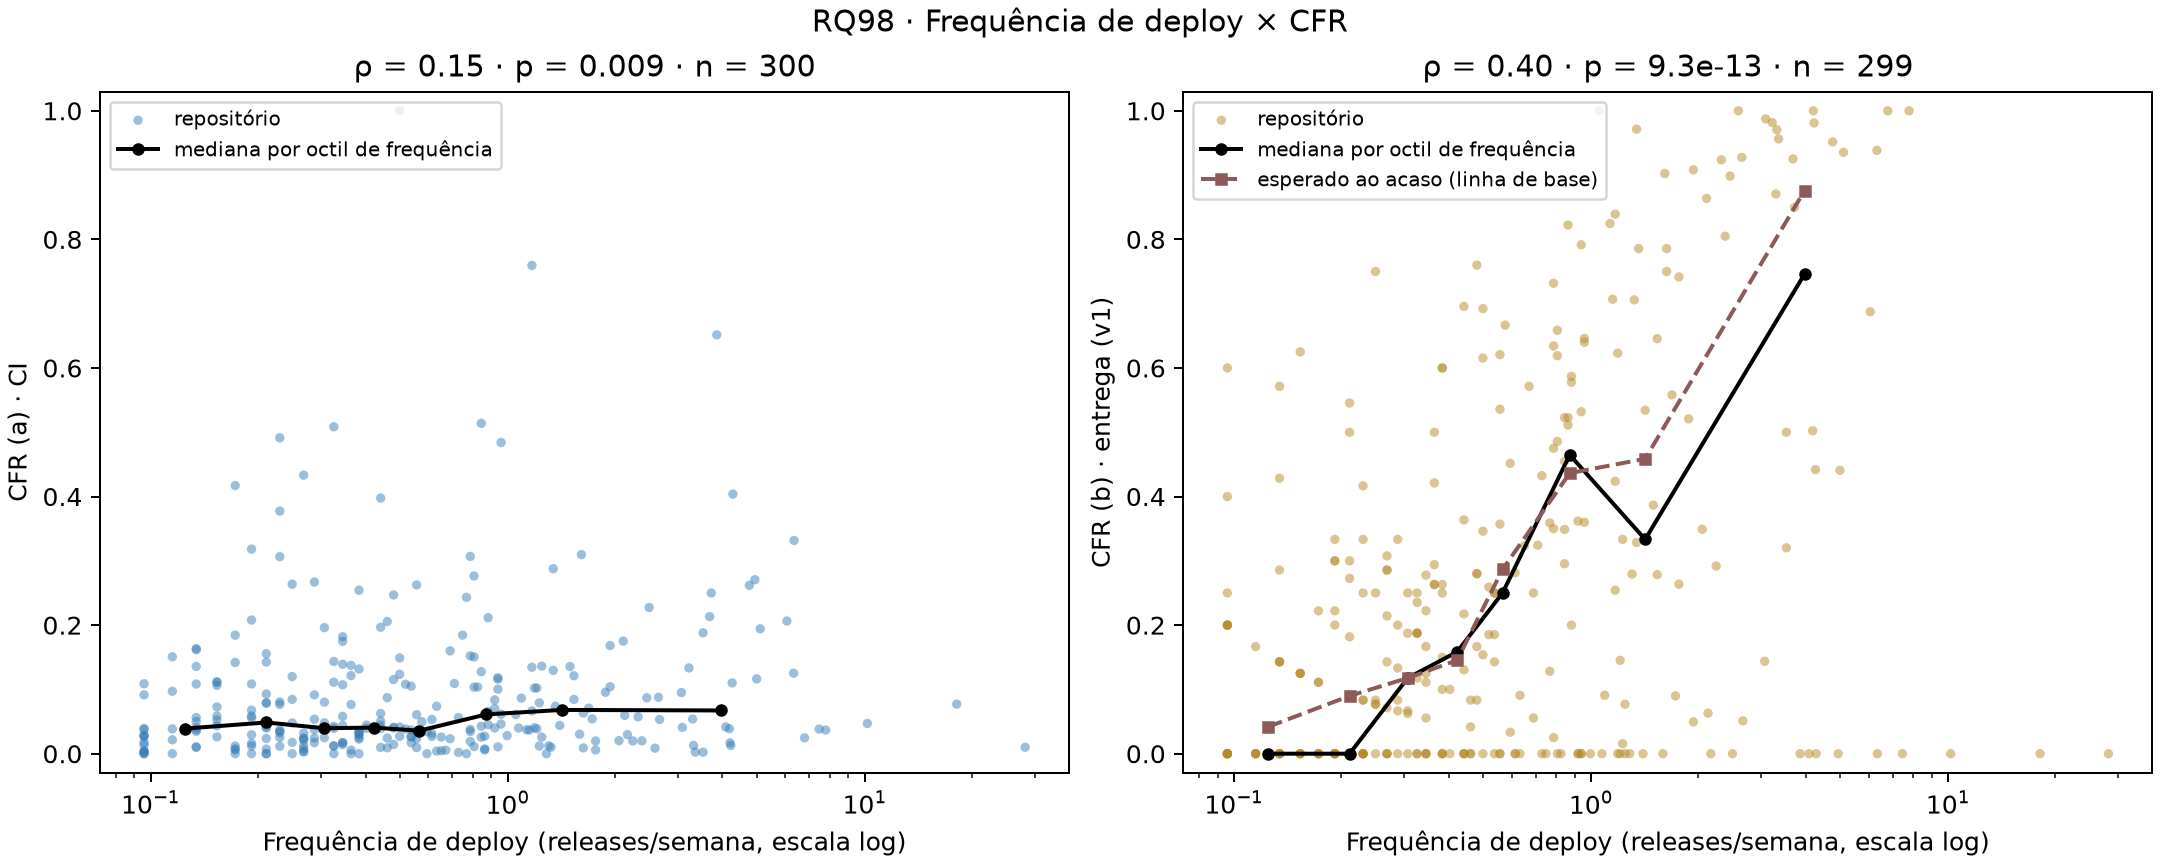
\includegraphics[width=0.95\linewidth]{figuras/dispersao_df_cfr.png}
\caption{Frequência de deploy (escala logarítmica) e CFR. Linha preta: mediana por octil de
frequência; linha tracejada: CFR (b) esperado ao acaso (linha de base da Seção~\ref{sec:discussao}).}
\label{fig:rq05}
\end{figure}

\subsection{RQ06 --- Características dos repositórios}
\label{sec:rq06}

\apreencher{resultados da RQ06 (issue \#93): Kruskal-Wallis ou Mann-Whitney por fator, p-valores
com correção de Holm, $\varepsilon^2$ e $\delta$ de Cliff}

\subsection{RQ07 --- Sensibilidade da classificação DORA}

Classificamos cada repositório em sete combinações de definições (C1 a C7, Tabela~\ref{tab:rq07}).
Dos 279 repositórios classificados em todas elas, 163 (58,4\%) têm a mesma classe geral em todas
e 116 (41,6\%) mudam em pelo menos uma alternativa à C1. Trocar só a unidade de deploy (C5 e C6)
muda de 3,6\% a 10,7\% das classes, sempre para melhor ($\kappa$ de 0,85 a 0,95); as
combinações com o CFR (b) mudam de 20,8\% a 35,5\%, e 75\% das mudanças são para pior. No nível
de cada métrica, trocar o CFR (a) pelo (b) muda a classe de 57,2\% dos repositórios
($\kappa = 0{,}02$), o \textit{lead time} (a) pelo (b), de 42,3\%, e a unidade de deploy de
release para tag, de 24,0\%.

\begin{table}[ht]
\centering
\small
\caption{Mudança da classe geral em relação à C1 (279 a 280 repositórios por par).}
\label{tab:rq07}
\begin{tabular}{llrrl}
\hline
Combinação & O que muda em relação à C1 & Mudam (\%) & $\kappa$ pond. & Landis--Koch \\
\hline
C2 & \textit{lead time} (b)                     & 14,3 & 0,79 & substancial \\
C3 & CFR (b)                                    & 20,8 & 0,68 & substancial \\
C4 & \textit{lead time} (b) e CFR (b)           & 29,7 & 0,52 & moderada \\
C5 & pré-releases contam como deploy            & 3,6  & 0,95 & quase perfeita \\
C6 & tags contam como deploy                    & 10,7 & 0,85 & quase perfeita \\
C7 & tags, \textit{lead time} (b) e CFR (b)     & 35,5 & 0,44 & moderada \\
\hline
\end{tabular}
\end{table}
 depois de % Secao 2 do artigo do LAB03 (template SBC). Issue #90.
% Uso no Overleaf: % Secao 2 do artigo do LAB03 (template SBC). Issue #90.
% Uso no Overleaf: \input{metodologia} depois de \input{introducao}.
% Requer os mesmos pacotes da introducao (nada alem do template).
%
% Trechos entre \apreencher{...} dependem de dados que ainda nao existem (amostra
% final de 300, rotulos humanos, consenso, F1) ou de confirmacao do professor
% (janela oficial). Nao ha numero inventado: o funil e o piloto da Sprint 01 sao
% identificados como tais. Busque por "apreencher" antes de entregar.

\providecommand{\apreencher}[1]{\textbf{[a preencher: #1]}}

\section{Metodologia}
\label{sec:metodologia}

\subsection{Visão geral}

O estudo calcula as quatro métricas DORA, a partir de dados públicos do GitHub,
para repositórios \textit{open-source} populares que usam GitHub Actions, e mede
a confiabilidade dessas medidas por duas vias: a validação manual das
heurísticas (Seção~\ref{sec:validacao}) e a análise de sensibilidade às
definições operacionais (RQ07). Todas as definições abaixo são comuns à turma,
para que os resultados sejam comparáveis e o pipeline possa ser replicado por
outro grupo (Seção~6).

\subsection{Fonte de dados e coleta}
\label{sec:coleta}

A coleta usa um cliente próprio das APIs REST e GraphQL do GitHub, sem
bibliotecas de acesso à API. A busca de candidatos (\texttt{GET
/search/repositories}) é fatiada por faixas de estrelas para contornar o teto de
1.000 resultados por consulta, e reúne 8.000 candidatos. Os metadados de cada
um (estrelas, linguagem principal, data de criação, \textit{default branch},
indicadores de \textit{fork}, arquivamento e repositório vazio) vêm da API
GraphQL. Para os repositórios aceitos, o pipeline coleta, pela API REST, as
releases (\texttt{/releases}), os \textit{commits} entre releases consecutivas
(\texttt{/compare}, com paginação para ultrapassar o limite de 250 \textit{commits}),
as tags e as execuções de \textit{workflow} (\texttt{/actions/runs}) do
\textit{default branch}.

Duas decisões de coleta afetam a validade. Primeiro, a busca de execuções
retorna no máximo 1.000 resultados por consulta; por isso a janela é consultada
mês a mês e qualquer intervalo que atinja o teto é dividido ao meio (até o
nível de segundos), de modo que nenhuma execução se perde sem aviso. Segundo, o
pipeline descarta repositórios com mais de 20.000 execuções na janela, por custo
de coleta; esse limite é contabilizado no funil e discutido como limitação.

A coleta é um pipeline reprodutível, executado por um único comando. Toda
resposta da API é gravada em disco (um arquivo por URL), o que permite retomar
uma coleta interrompida sem repetir chamadas. O cliente lê os cabeçalhos
\texttt{X-RateLimit-Remaining} e \texttt{X-RateLimit-Reset} e espera
sozinho quando a cota acaba. Erros temporários (respostas 5xx e quedas de rede)
são repetidos com \textit{backoff} exponencial (1~s, 2~s, 4~s, \ldots, até 60~s,
em até 6 tentativas). O \textit{token} vem de variável de ambiente e nunca é
versionado. As funções que calculam as métricas têm testes automatizados
(\textit{pytest}, cobertura mínima de 80\% do módulo de métricas, medida com
\textit{pytest-cov}) executados no GitHub Actions do grupo a cada \textit{push}.

\subsection{Seleção da amostra e funil}
\label{sec:funil}

Os candidatos são avaliados em ordem decrescente de estrelas, do critério mais
barato ao mais caro, até se atingir a meta de pelo menos 300 repositórios. Um
repositório entra na amostra se (i) não é \textit{fork}, está ativo (não
arquivado, desabilitado ou vazio) e tem \textit{default branch}; (ii) usa GitHub
Actions (\texttt{total\_count > 0} em \texttt{/actions/workflows}); (iii) tem
pelo menos 5 releases publicadas na janela; e (iv) tem pelo menos 50 execuções
válidas no \textit{default branch} na janela. Os critérios não são relaxados para
atingir a meta. A Tabela~\ref{tab:funil} mostra o funil; as colunas trazem o
piloto da primeira sprint (meta de 100) e a amostra final.

\begin{table}[ht]
\centering
\small
\caption{Funil de seleção. O piloto (Sprint 01) foi coletado com a janela
provisória; a amostra final ainda não foi exportada.}
\label{tab:funil}
\begin{tabular}{lrr}
\hline
Etapa & Piloto ($n=100$) & Final \\
\hline
Candidatos com metadados & 8.000 & \apreencher{n} \\
Ativos (sem \textit{fork}/arquivados/vazios) & 7.519 & \apreencher{n} \\
Avaliados até a meta & 272 & \apreencher{n} \\
Usam GitHub Actions & 253 & \apreencher{n} \\
$\geq 5$ releases na janela & 132 & \apreencher{n} \\
$\leq 20.000$ execuções (custo) & 114 & \apreencher{n} \\
$\geq 50$ execuções válidas & 100 & \apreencher{$\geq 300$} \\
\hline
\end{tabular}
\end{table}

\subsection{Definições operacionais}
\label{sec:definicoes}

\begin{table}[ht]
\centering
\small
\caption{Definições operacionais comuns à turma.}
\label{tab:definicoes}
\begin{tabular}{p{0.22\linewidth}p{0.68\linewidth}}
\hline
Elemento & Definição \\
\hline
Janela & 12 meses, de 01/10/2025 a 30/09/2026, com as duas datas inclusivas
\apreencher{confirmar a janela oficial com o professor} \\
\textit{Branch} & Apenas o \textit{default branch} (\texttt{default\_branch}) \\
Deploy & Release publicada (\texttt{draft = false}) e não pré-release;
pré-releases e tags são variantes da RQ07 \\
Data do \textit{commit} & \texttt{commit.author.date} \\
Execução de CI & \textit{Workflow run} do \textit{default branch} com
\texttt{event = push}, criado na janela \\
Sucesso & \texttt{success} \\
Falha & \texttt{failure}, \texttt{timed\_out}, \texttt{startup\_failure} \\
Ignorada & \texttt{cancelled}, \texttt{skipped}, \texttt{neutral},
\texttt{action\_required}, \texttt{stale} ou vazio \\
Censura & Evento final não observado na janela: registrado como censurado, não
descartado \\
\hline
\end{tabular}
\end{table}

\subsection{Métricas e variantes}
\label{sec:metricas}

Em todas as RQs reportamos mediana e intervalo interquartil (IQR, quartis por
interpolação linear), e não média e desvio-padrão, porque as distribuições são
assimétricas.

\textbf{RQ01 -- Frequência de deploy.} Releases publicadas na janela divididas
pelo número de semanas da janela ($\approx 52{,}1$).

\textbf{RQ02 -- \textit{Lead time}.} Para cada release R da janela, os
\textit{commits} são os do \texttt{compare} com a release publicada
imediatamente anterior, que pode estar fora da janela. Na variante (a), o
\textit{lead time} de R é a data de R menos a do \textit{commit} mais antigo, e o
valor do repositório é a mediana entre as releases. Na variante (b), cada
\textit{commit} contribui com a data de R menos a sua, e o valor do repositório é
a mediana de todos os \textit{commits} de todas as releases (e não uma mediana de
medianas). Decisões do grupo: a primeira release da história do repositório é
ignorada; \texttt{compare} indisponível (por exemplo, tag apagada) ou truncado
exclui a release do cálculo e é contado; uma release sem \textit{commits} novos
fica fora das duas variantes; e um \textit{commit} com data de autoria posterior
à da release (relógio errado ou tag movida) é descartado e contado.

\textbf{RQ03 -- Taxa de falha (CFR).} A variante (a), de CI, é o número de
execuções com falha dividido por falhas mais sucessos, considerando todos os
\textit{workflows} juntos; ela mede falha de pipeline, não de produção. A
variante (b), de entrega, considera uma release R como falha se for seguida, em
até 7 dias (inclusive), por uma release corretiva; o CFR é o número de releases
que falharam dividido pelo de avaliadas. Várias corretivas na semana não
multiplicam a falha de R. Releases dos últimos 7 dias da janela são censuradas e
ficam fora do denominador.

\textbf{RQ04 -- Tempo de recuperação.} Dentro de cada \textit{workflow}, um
episódio de falha começa na primeira falha após um sucesso e termina no próximo
sucesso; sua duração é o \texttt{updated\_at} do sucesso menos o
\texttt{run\_started\_at} da falha. Execuções ignoradas não interrompem nem
iniciam episódios. O valor do repositório é a mediana dos episódios de todos os
seus \textit{workflows}. Episódios sem sucesso até o fim da janela são
censurados à direita. Por decisão do grupo, também são censurados (à esquerda)
os episódios de um \textit{workflow} cuja primeira execução válida na janela já
é uma falha, pois o início real é desconhecido. Episódios censurados não entram
na mediana, e a proporção deles é reportada por repositório. Repositório sem
falhas tem recuperação indefinida (e não zero).

\textbf{Classificação DORA.} Cada métrica recebe 4 (Elite), 3 (High), 2 (Medium)
ou 1 (Low) pelos cortes fixos da disciplina; a categoria geral é a mediana dos
quatro valores, arredondada para baixo.

\subsection{Heurística de release corretiva}
\label{sec:heuristica}

Uma release é corretiva quando seu objetivo principal é corrigir um defeito
recente. Como o GitHub não registra isso, usamos heurísticas sobre a tag e sobre
a primeira linha das mensagens dos \textit{commits} entre a release anterior e a
avaliada. Testamos três versões, aplicadas sempre em relação à release publicada
imediatamente anterior:

\begin{itemize}
  \item \textbf{v1 (\textit{patch} SemVer):} só o número de \textit{patch}
  mudou (por exemplo, $2.3.0 \rightarrow 2.3.1$). Tags que não seguem SemVer
  estrito, pré-releases e \textit{downgrades} nunca são corretivas.
  \item \textbf{v2 (\textit{patch} ou mensagem):} v1, ou algum \textit{commit}
  com \texttt{revert}, \texttt{hotfix} ou \texttt{fix}.
  \item \textbf{v3 (correção de defeito):} \texttt{revert} ou \texttt{hotfix}
  bastam; caso contrário, exige \textit{commit} \texttt{fix} que não trate de
  \textit{typo}, documentação, CI, testes ou dependências, e que o \textit{patch}
  tenha mudado ou que ao menos metade dos \textit{commits} (sem \textit{merges}) seja
  correção, sem \textit{commit} de funcionalidade. Sem mensagens disponíveis,
  vale só a tag.
\end{itemize}

A versão usada no CFR (b) é a que atingir F1~$\geq 0{,}70$ contra o consenso
da amostra-ouro; se nenhuma atingir, a heurística é refinada e reavaliada, e
todas as versões e seus F1 são reportadas. Resultados:
\apreencher{P, R e F1 de v1, v2, v3 e das versões seguintes}.
As heurísticas não leem as \textit{release notes} nem o \textit{diff}; isso é
uma limitação.

\subsection{Validação manual (amostra-ouro)}
\label{sec:validacao}

Sorteamos 60 repositórios da amostra final com \texttt{df.sample(n=60,
random\_state=42)}, sobre a amostra ordenada por nome (a ordem do arquivo não
altera o sorteio), e, em cada um, até 5 releases da definição principal de
deploy que tenham release anterior (a primeira da história fica de fora, pois
não há lista de \textit{commits} para ler). Os três integrantes rotularam, de
forma independente, sem consultar os demais e sem ver a saída da heurística, em
planilhas idênticas com ligações para a página da release e para o
\texttt{compare}: (i)~o tipo do projeto (biblioteca/\textit{framework},
aplicação/serviço, ferramenta CLI ou outro); (ii)~se as releases representam
entregas reais ao usuário (sim, não ou incerto); e (iii)~se cada release
sorteada é corretiva (sim ou não).

A concordância entre os três avaliadores é medida com o $\kappa$ de Fleiss em
cada dimensão (interpretação de Landis e Koch). Os casos divergentes são
discutidos pelo grupo e geram o rótulo de consenso; o protocolo de desempate é
\apreencher{protocolo definido na consolidação do consenso}. Um $\kappa$ baixo é
tratado como achado sobre a ambiguidade do critério. A heurística é avaliada
contra o consenso com precisão, \textit{recall} e F1 (classe positiva:
corretiva). Como as regras são ajustadas olhando os erros desta mesma amostra, o
F1 final tende a ser otimista. Resultados: \apreencher{$\kappa$ por dimensão,
tamanho do consenso}. O tipo do projeto rotulado alimenta a RQ06.

\subsection{Análise estatística}
\label{sec:analise}

Para a RQ05, usamos a correlação de Spearman ($\rho$, p-valor e $n$) entre a
frequência de deploy e o CFR, separadamente para as variantes (a) e (b). Na RQ06,
comparamos as métricas entre subgrupos de pelo menos três fatores (linguagem,
quartis de estrelas, de contribuidores e de idade, e tipo do projeto) com
Kruskal-Wallis (ou Mann-Whitney, quando há dois grupos), corrigimos os p-valores
por Holm e reportamos o tamanho de efeito ($\varepsilon^2 = H/(n-1)$ ou
$\delta$ de Cliff). Na RQ07, montamos ao menos três combinações de definições
(por exemplo, release, release com pré-release e tag como unidade de deploy,
combinadas com as variantes de \textit{lead time} e de CFR), classificamos cada
repositório em cada combinação e calculamos, por par, a proporção que muda de
categoria e o $\kappa$ de Cohen ponderado (pesos lineares).

\subsection{Disponibilidade}

O código, os testes, o dicionário de dados e os CSVs finais estão no
repositório do grupo (Seção~7). O pipeline é executável por outro grupo com um
único comando, conforme o README.
 depois de % Secao 1 do artigo do LAB03 (template SBC). Issue #81.
% Uso no Overleaf: \input{introducao} no corpo e \bibliography{referencias}
% com \bibliographystyle{sbc}. Requer \usepackage[utf8]{inputenc} (ja no template).
% Hipoteses registradas antes da analise dos dados.

\section{Introdução}
\label{sec:introducao}

Medir o desempenho de entrega de software é um problema antigo da engenharia de
software. Nos últimos anos ele ganhou um vocabulário comum com as métricas DORA
(\textit{DevOps Research and Assessment}). Popularizadas pelo livro
\textit{Accelerate}~\cite{forsgren2018accelerate} e atualizadas anualmente pelos
relatórios \textit{State of DevOps}~\cite{dora2024report}, elas descrevem a
entrega em duas dimensões. A \textbf{velocidade} é medida pela frequência de
deploy e pelo \textit{lead time for changes}. A \textbf{estabilidade} é medida
pela taxa de falha das mudanças (\textit{change failure rate}, CFR) e pelo tempo
de recuperação após um deploy com falha~\cite{dora2024fourkeys}. Um dos achados
mais citados dessa linha de pesquisa é que velocidade e estabilidade
\textbf{não} seriam um \textit{trade-off}: as equipes de melhor desempenho iriam
bem nas duas dimensões ao mesmo tempo.

Esses resultados vêm, na maior parte, de questionários respondidos por
profissionais de empresas. Em projetos open-source, os dados de entrega são
públicos e podem ser \textbf{minerados}: releases, \textit{commits} e execuções de
integração contínua (CI) no GitHub Actions ficam registrados com data e
resultado. O GitHub, porém, não registra ``deploys em produção'' nem ``falhas em
produção''. Cada métrica DORA precisa então ser aproximada por um
\textbf{proxy}. Uma release publicada faz o papel de deploy, e uma execução de CI
com falha, ou uma release corretiva logo em seguida, faz o papel de falha.
Proxies podem enganar. Uma biblioteca que publica uma release por mês não está
``deployando'' nada; quem faz isso são os usuários dela. Um \textit{workflow} de
CI vermelho indica falha de pipeline, e não necessariamente um defeito que
chegou ao usuário.

Este trabalho minera as métricas DORA de repositórios open-source populares que
usam CI/CD com GitHub Actions. Ele tem dois objetivos. O primeiro é
\textbf{descrever} o desempenho de entrega desses projetos sob definições
operacionais comuns: janela de 12 meses, \textit{default branch}, releases
não-\textit{draft} e execuções disparadas por \texttt{push}. O segundo é
\textbf{avaliar o quanto essas medidas são confiáveis}. Para isso, (i) validamos
as heurísticas automáticas contra uma amostra rotulada manualmente por três
avaliadores independentes e (ii) medimos o quanto a classificação DORA de cada
repositório muda quando a definição operacional muda (análise de
sensibilidade). Investigamos as seguintes questões de pesquisa:

\begin{itemize}
  \item \textbf{RQ01.} Qual a frequência de deploys dos repositórios populares que usam CI/CD?
  \item \textbf{RQ02.} Qual o tempo entre um \textit{commit} e seu respectivo deploy, por release e por \textit{commit}?
  \item \textbf{RQ03.} Qual a taxa de falha das mudanças entregues, pelo proxy de CI e pelo proxy de entrega?
  \item \textbf{RQ04.} Qual o tempo de recuperação após uma execução de CI/CD com falha?
  \item \textbf{RQ05.} Repositórios com maior frequência de deploy apresentam maior ou menor taxa de falha?
  \item \textbf{RQ06.} Quais características dos repositórios estão associadas a um melhor desempenho DORA?
  \item \textbf{RQ07.} O quanto a classificação DORA de um repositório depende da definição operacional escolhida?
\end{itemize}

O pipeline de coleta foi escrito pelo grupo, sem bibliotecas de acesso à API do
GitHub. Ele é executável com um único comando, tem cache e retomada, é coberto
por testes automatizados que rodam no GitHub Actions do próprio grupo e será
replicado por outro grupo da turma. A Seção~2 descreve a metodologia; a
Seção~3 apresenta os resultados; a Seção~4 discute as hipóteses frente aos
resultados; a Seção~5 trata das ameaças à validade; e a Seção~6 relata a
replicação cruzada.

\subsection{Hipóteses informais}
\label{sec:hipoteses}

Para cada RQ registramos, antes da análise dos dados, o que esperamos encontrar
e por quê. As faixas Elite/High/Medium/Low seguem a tabela de referência da
disciplina.

\begin{description}
  \item[H1 (RQ01).] Mediana da ordem de uma release a cada uma ou duas semanas
  ($\approx$0,5 a 1 release/semana), concentrando os repositórios nas faixas
  Medium e High, com cauda longa à direita e poucos repositórios Elite (releases
  automatizadas, \textit{nightlies}, \textit{monorepos}). Mesmo após o critério
  de inclusão ($\geq$5 releases), projetos open-source agrupam mudanças em
  versões, porque cada release tem custo para quem a consome.

  \item[H2 (RQ02).] O lead time por release (a) terá mediana na faixa de semanas
  (Medium, muitas vezes Low), e o lead time por \textit{commit} (b) será
  sistematicamente menor, na faixa de dias. A variante (a) é definida pelo
  \textit{commit} mais antigo da release, então um único \textit{commit}
  ``esquecido'' (\textit{branch} longo, \textit{cherry-pick}, \textit{rebase} que
  preserva a data de autoria) a faz explodir; a (b) dilui esse \textit{commit}.
  A diferença entre (a) e (b) deve crescer com o tamanho das releases.

  \item[H3 (RQ03).] CFR de CI (a) mediano entre 10\% e 25\% (Elite/High), por
  testes instáveis e quebras corrigidas no \textit{commit} seguinte, atenuadas
  pela proteção do \textit{default branch}. CFR de entrega (b) menor, entre 5\% e
  15\%, porém mais variável. Correlação fraca entre (a) e (b) ($|\rho|<0{,}3$),
  porque as duas medem fenômenos diferentes: fragilidade do pipeline e defeitos
  que escaparam até a release.

  \item[H4 (RQ04).] Tempo de recuperação mediano de algumas horas (entre 1 hora e
  1 dia, High): uma quebra no \textit{default branch} bloqueia os colaboradores e
  tende a ser corrigida no mesmo dia. Distribuição assimétrica, com cauda de
  episódios longos em \textit{workflows} secundários. Proporção de episódios
  censurados abaixo de 10\%.

  \item[H5 (RQ05).] Ausência de \textit{trade-off}: correlação de Spearman
  próxima de zero ou levemente negativa entre frequência de deploy e CFR (b), em
  linha com o DORA, e próxima de zero para o CFR (a). Mais releases tendem a vir
  acompanhadas de mais automação. Uma correlação fraca não implica causalidade e
  pode refletir fatores de confusão, como tamanho da equipe e maturidade.

  \item[H6 (RQ06).] Repositórios com mais contribuidores terão maior frequência de
  deploy e menor tempo de recuperação, mas CFR (a) maior. Bibliotecas e
  frameworks terão lead time maior e frequência menor que ferramentas CLI e
  aplicações, pela exigência de estabilidade de API. A linguagem principal estará
  associada à frequência de deploy. Os efeitos devem ser pequenos a médios
  ($\varepsilon^2<0{,}06$ na maioria) e parte deles deve perder significância
  após a correção de Holm. Estrelas terão efeito desprezível.

  \item[H7 (RQ07).] A classificação DORA será frágil: pelo menos 30\% dos
  repositórios mudarão de categoria geral entre a combinação de referência e as
  alternativas, com kappa de Cohen ponderado entre 0,2 e 0,6. Pré-releases e
  tags devem inflar a frequência de deploy, e trocar o lead time (a) pelo (b)
  deve melhorar a classe de muitos repositórios. Se confirmada, as conclusões
  das RQ01 a RQ06 devem ser lidas como condicionais à definição operacional.
\end{description}
.
% Requer os mesmos pacotes da introducao (nada alem do template).
%
% Trechos entre \apreencher{...} dependem de dados que ainda nao existem (amostra
% final de 300, rotulos humanos, consenso, F1) ou de confirmacao do professor
% (janela oficial). Nao ha numero inventado: o funil e o piloto da Sprint 01 sao
% identificados como tais. Busque por "apreencher" antes de entregar.

\providecommand{\apreencher}[1]{\textbf{[a preencher: #1]}}

\section{Metodologia}
\label{sec:metodologia}

\subsection{Visão geral}

O estudo calcula as quatro métricas DORA, a partir de dados públicos do GitHub,
para repositórios \textit{open-source} populares que usam GitHub Actions, e mede
a confiabilidade dessas medidas por duas vias: a validação manual das
heurísticas (Seção~\ref{sec:validacao}) e a análise de sensibilidade às
definições operacionais (RQ07). Todas as definições abaixo são comuns à turma,
para que os resultados sejam comparáveis e o pipeline possa ser replicado por
outro grupo (Seção~6).

\subsection{Fonte de dados e coleta}
\label{sec:coleta}

A coleta usa um cliente próprio das APIs REST e GraphQL do GitHub, sem
bibliotecas de acesso à API. A busca de candidatos (\texttt{GET
/search/repositories}) é fatiada por faixas de estrelas para contornar o teto de
1.000 resultados por consulta, e reúne 8.000 candidatos. Os metadados de cada
um (estrelas, linguagem principal, data de criação, \textit{default branch},
indicadores de \textit{fork}, arquivamento e repositório vazio) vêm da API
GraphQL. Para os repositórios aceitos, o pipeline coleta, pela API REST, as
releases (\texttt{/releases}), os \textit{commits} entre releases consecutivas
(\texttt{/compare}, com paginação para ultrapassar o limite de 250 \textit{commits}),
as tags e as execuções de \textit{workflow} (\texttt{/actions/runs}) do
\textit{default branch}.

Duas decisões de coleta afetam a validade. Primeiro, a busca de execuções
retorna no máximo 1.000 resultados por consulta; por isso a janela é consultada
mês a mês e qualquer intervalo que atinja o teto é dividido ao meio (até o
nível de segundos), de modo que nenhuma execução se perde sem aviso. Segundo, o
pipeline descarta repositórios com mais de 20.000 execuções na janela, por custo
de coleta; esse limite é contabilizado no funil e discutido como limitação.

A coleta é um pipeline reprodutível, executado por um único comando. Toda
resposta da API é gravada em disco (um arquivo por URL), o que permite retomar
uma coleta interrompida sem repetir chamadas. O cliente lê os cabeçalhos
\texttt{X-RateLimit-Remaining} e \texttt{X-RateLimit-Reset} e espera
sozinho quando a cota acaba. Erros temporários (respostas 5xx e quedas de rede)
são repetidos com \textit{backoff} exponencial (1~s, 2~s, 4~s, \ldots, até 60~s,
em até 6 tentativas). O \textit{token} vem de variável de ambiente e nunca é
versionado. As funções que calculam as métricas têm testes automatizados
(\textit{pytest}, cobertura mínima de 80\% do módulo de métricas, medida com
\textit{pytest-cov}) executados no GitHub Actions do grupo a cada \textit{push}.

\subsection{Seleção da amostra e funil}
\label{sec:funil}

Os candidatos são avaliados em ordem decrescente de estrelas, do critério mais
barato ao mais caro, até se atingir a meta de pelo menos 300 repositórios. Um
repositório entra na amostra se (i) não é \textit{fork}, está ativo (não
arquivado, desabilitado ou vazio) e tem \textit{default branch}; (ii) usa GitHub
Actions (\texttt{total\_count > 0} em \texttt{/actions/workflows}); (iii) tem
pelo menos 5 releases publicadas na janela; e (iv) tem pelo menos 50 execuções
válidas no \textit{default branch} na janela. Os critérios não são relaxados para
atingir a meta. A Tabela~\ref{tab:funil} mostra o funil; as colunas trazem o
piloto da primeira sprint (meta de 100) e a amostra final.

\begin{table}[ht]
\centering
\small
\caption{Funil de seleção. O piloto (Sprint 01) foi coletado com a janela
provisória; a amostra final ainda não foi exportada.}
\label{tab:funil}
\begin{tabular}{lrr}
\hline
Etapa & Piloto ($n=100$) & Final \\
\hline
Candidatos com metadados & 8.000 & \apreencher{n} \\
Ativos (sem \textit{fork}/arquivados/vazios) & 7.519 & \apreencher{n} \\
Avaliados até a meta & 272 & \apreencher{n} \\
Usam GitHub Actions & 253 & \apreencher{n} \\
$\geq 5$ releases na janela & 132 & \apreencher{n} \\
$\leq 20.000$ execuções (custo) & 114 & \apreencher{n} \\
$\geq 50$ execuções válidas & 100 & \apreencher{$\geq 300$} \\
\hline
\end{tabular}
\end{table}

\subsection{Definições operacionais}
\label{sec:definicoes}

\begin{table}[ht]
\centering
\small
\caption{Definições operacionais comuns à turma.}
\label{tab:definicoes}
\begin{tabular}{p{0.22\linewidth}p{0.68\linewidth}}
\hline
Elemento & Definição \\
\hline
Janela & 12 meses, de 01/10/2025 a 30/09/2026, com as duas datas inclusivas
\apreencher{confirmar a janela oficial com o professor} \\
\textit{Branch} & Apenas o \textit{default branch} (\texttt{default\_branch}) \\
Deploy & Release publicada (\texttt{draft = false}) e não pré-release;
pré-releases e tags são variantes da RQ07 \\
Data do \textit{commit} & \texttt{commit.author.date} \\
Execução de CI & \textit{Workflow run} do \textit{default branch} com
\texttt{event = push}, criado na janela \\
Sucesso & \texttt{success} \\
Falha & \texttt{failure}, \texttt{timed\_out}, \texttt{startup\_failure} \\
Ignorada & \texttt{cancelled}, \texttt{skipped}, \texttt{neutral},
\texttt{action\_required}, \texttt{stale} ou vazio \\
Censura & Evento final não observado na janela: registrado como censurado, não
descartado \\
\hline
\end{tabular}
\end{table}

\subsection{Métricas e variantes}
\label{sec:metricas}

Em todas as RQs reportamos mediana e intervalo interquartil (IQR, quartis por
interpolação linear), e não média e desvio-padrão, porque as distribuições são
assimétricas.

\textbf{RQ01 -- Frequência de deploy.} Releases publicadas na janela divididas
pelo número de semanas da janela ($\approx 52{,}1$).

\textbf{RQ02 -- \textit{Lead time}.} Para cada release R da janela, os
\textit{commits} são os do \texttt{compare} com a release publicada
imediatamente anterior, que pode estar fora da janela. Na variante (a), o
\textit{lead time} de R é a data de R menos a do \textit{commit} mais antigo, e o
valor do repositório é a mediana entre as releases. Na variante (b), cada
\textit{commit} contribui com a data de R menos a sua, e o valor do repositório é
a mediana de todos os \textit{commits} de todas as releases (e não uma mediana de
medianas). Decisões do grupo: a primeira release da história do repositório é
ignorada; \texttt{compare} indisponível (por exemplo, tag apagada) ou truncado
exclui a release do cálculo e é contado; uma release sem \textit{commits} novos
fica fora das duas variantes; e um \textit{commit} com data de autoria posterior
à da release (relógio errado ou tag movida) é descartado e contado.

\textbf{RQ03 -- Taxa de falha (CFR).} A variante (a), de CI, é o número de
execuções com falha dividido por falhas mais sucessos, considerando todos os
\textit{workflows} juntos; ela mede falha de pipeline, não de produção. A
variante (b), de entrega, considera uma release R como falha se for seguida, em
até 7 dias (inclusive), por uma release corretiva; o CFR é o número de releases
que falharam dividido pelo de avaliadas. Várias corretivas na semana não
multiplicam a falha de R. Releases dos últimos 7 dias da janela são censuradas e
ficam fora do denominador.

\textbf{RQ04 -- Tempo de recuperação.} Dentro de cada \textit{workflow}, um
episódio de falha começa na primeira falha após um sucesso e termina no próximo
sucesso; sua duração é o \texttt{updated\_at} do sucesso menos o
\texttt{run\_started\_at} da falha. Execuções ignoradas não interrompem nem
iniciam episódios. O valor do repositório é a mediana dos episódios de todos os
seus \textit{workflows}. Episódios sem sucesso até o fim da janela são
censurados à direita. Por decisão do grupo, também são censurados (à esquerda)
os episódios de um \textit{workflow} cuja primeira execução válida na janela já
é uma falha, pois o início real é desconhecido. Episódios censurados não entram
na mediana, e a proporção deles é reportada por repositório. Repositório sem
falhas tem recuperação indefinida (e não zero).

\textbf{Classificação DORA.} Cada métrica recebe 4 (Elite), 3 (High), 2 (Medium)
ou 1 (Low) pelos cortes fixos da disciplina; a categoria geral é a mediana dos
quatro valores, arredondada para baixo.

\subsection{Heurística de release corretiva}
\label{sec:heuristica}

Uma release é corretiva quando seu objetivo principal é corrigir um defeito
recente. Como o GitHub não registra isso, usamos heurísticas sobre a tag e sobre
a primeira linha das mensagens dos \textit{commits} entre a release anterior e a
avaliada. Testamos três versões, aplicadas sempre em relação à release publicada
imediatamente anterior:

\begin{itemize}
  \item \textbf{v1 (\textit{patch} SemVer):} só o número de \textit{patch}
  mudou (por exemplo, $2.3.0 \rightarrow 2.3.1$). Tags que não seguem SemVer
  estrito, pré-releases e \textit{downgrades} nunca são corretivas.
  \item \textbf{v2 (\textit{patch} ou mensagem):} v1, ou algum \textit{commit}
  com \texttt{revert}, \texttt{hotfix} ou \texttt{fix}.
  \item \textbf{v3 (correção de defeito):} \texttt{revert} ou \texttt{hotfix}
  bastam; caso contrário, exige \textit{commit} \texttt{fix} que não trate de
  \textit{typo}, documentação, CI, testes ou dependências, e que o \textit{patch}
  tenha mudado ou que ao menos metade dos \textit{commits} (sem \textit{merges}) seja
  correção, sem \textit{commit} de funcionalidade. Sem mensagens disponíveis,
  vale só a tag.
\end{itemize}

A versão usada no CFR (b) é a que atingir F1~$\geq 0{,}70$ contra o consenso
da amostra-ouro; se nenhuma atingir, a heurística é refinada e reavaliada, e
todas as versões e seus F1 são reportadas. Resultados:
\apreencher{P, R e F1 de v1, v2, v3 e das versões seguintes}.
As heurísticas não leem as \textit{release notes} nem o \textit{diff}; isso é
uma limitação.

\subsection{Validação manual (amostra-ouro)}
\label{sec:validacao}

Sorteamos 60 repositórios da amostra final com \texttt{df.sample(n=60,
random\_state=42)}, sobre a amostra ordenada por nome (a ordem do arquivo não
altera o sorteio), e, em cada um, até 5 releases da definição principal de
deploy que tenham release anterior (a primeira da história fica de fora, pois
não há lista de \textit{commits} para ler). Os três integrantes rotularam, de
forma independente, sem consultar os demais e sem ver a saída da heurística, em
planilhas idênticas com ligações para a página da release e para o
\texttt{compare}: (i)~o tipo do projeto (biblioteca/\textit{framework},
aplicação/serviço, ferramenta CLI ou outro); (ii)~se as releases representam
entregas reais ao usuário (sim, não ou incerto); e (iii)~se cada release
sorteada é corretiva (sim ou não).

A concordância entre os três avaliadores é medida com o $\kappa$ de Fleiss em
cada dimensão (interpretação de Landis e Koch). Os casos divergentes são
discutidos pelo grupo e geram o rótulo de consenso; o protocolo de desempate é
\apreencher{protocolo definido na consolidação do consenso}. Um $\kappa$ baixo é
tratado como achado sobre a ambiguidade do critério. A heurística é avaliada
contra o consenso com precisão, \textit{recall} e F1 (classe positiva:
corretiva). Como as regras são ajustadas olhando os erros desta mesma amostra, o
F1 final tende a ser otimista. Resultados: \apreencher{$\kappa$ por dimensão,
tamanho do consenso}. O tipo do projeto rotulado alimenta a RQ06.

\subsection{Análise estatística}
\label{sec:analise}

Para a RQ05, usamos a correlação de Spearman ($\rho$, p-valor e $n$) entre a
frequência de deploy e o CFR, separadamente para as variantes (a) e (b). Na RQ06,
comparamos as métricas entre subgrupos de pelo menos três fatores (linguagem,
quartis de estrelas, de contribuidores e de idade, e tipo do projeto) com
Kruskal-Wallis (ou Mann-Whitney, quando há dois grupos), corrigimos os p-valores
por Holm e reportamos o tamanho de efeito ($\varepsilon^2 = H/(n-1)$ ou
$\delta$ de Cliff). Na RQ07, montamos ao menos três combinações de definições
(por exemplo, release, release com pré-release e tag como unidade de deploy,
combinadas com as variantes de \textit{lead time} e de CFR), classificamos cada
repositório em cada combinação e calculamos, por par, a proporção que muda de
categoria e o $\kappa$ de Cohen ponderado (pesos lineares).

\subsection{Disponibilidade}

O código, os testes, o dicionário de dados e os CSVs finais estão no
repositório do grupo (Seção~7). O pipeline é executável por outro grupo com um
único comando, conforme o README.
; as figuras ficam em figuras/
% (\usepackage{graphicx}, ja no template).
%
% Todos os numeros vem das analises do repositorio (entregas/laboratorio-03/sprint-03):
% RQ91 (RQ01), RQ94 (RQ02), RQ97 (RQ03), RQ92 (RQ04), RQ95 (classificacao C1),
% RQ98 (RQ05), RQ96 (RQ07). Janela provisoria; CFR (b) com a heuristica v1, ainda sem F1 medido.
% Trechos em \apreencher{...} dependem de analises ainda nao feitas (RQ06, issue #93) ou da
% validacao manual (issues #85 a #89). Busque por "apreencher" antes de entregar.

\providecommand{\apreencher}[1]{\textbf{[a preencher: #1]}}

\section{Resultados}
\label{sec:resultados}

Os resultados se referem aos 300 repositórios da amostra final (Seção~\ref{sec:funil}),
na janela de 01/10/2025 a 30/09/2026, ainda provisória (Seção~\ref{sec:definicoes}). Cada
repositório tem o mesmo peso e a estatística da amostra é a mediana dos valores dos
repositórios, com o intervalo interquartil (IQR, Q1--Q3). A Tabela~\ref{tab:descritivo} resume
as métricas e a classificação DORA de cada uma. Nas Seções~\ref{sec:rq03} e~\ref{sec:rq05},
o CFR (b) usa a versão v1 da heurística de release corretiva, que ainda não tem F1 medido
contra o consenso da amostra-ouro (\apreencher{P, R e F1 das versões v1, v2 e v3}).

\begin{table}[ht]
\centering
\small
\caption{Métricas DORA e classes (\% dos repositórios com a métrica definida). Frequência em
releases/semana; \textit{lead time} em dias; CFR em \%; recuperação em horas.}
\label{tab:descritivo}
\begin{tabular}{lrrrrrr}
\hline
Métrica & $n$ & Mediana (Q1--Q3) & Elite & High & Medium & Low \\
\hline
Frequência de deploy      & 300 & 0,48 (0,23--1,16) & 1,7  & 25,0 & 50,7 & 22,7 \\
\textit{Lead time} (a)    & 300 & 10,5 (3,6--39,5)  & 14,3 & 25,0 & 30,3 & 30,3 \\
\textit{Lead time} (b)    & 300 & 12,1 (3,3--57,5)  & 10,3 & 28,7 & 28,7 & 32,3 \\
CFR (a), CI               & 300 & 4,6 (2,3--11,1)   & 83,0 & 11,3 & 3,3  & 2,3  \\
CFR (b), entrega (v1)     & 299 & 18,8 (0,0--44,7)  & 47,5 & 18,4 & 9,0  & 25,1 \\
Recuperação               & 280 & 2,7 (1,1--6,9)    & 23,2 & 66,4 & 9,3  & 1,1  \\
\hline
Classe geral (C1)         & 280 & ---               & 6,4  & 43,6 & 45,7 & 4,3  \\
\hline
\end{tabular}
\end{table}

\begin{figure}[ht]
\centering
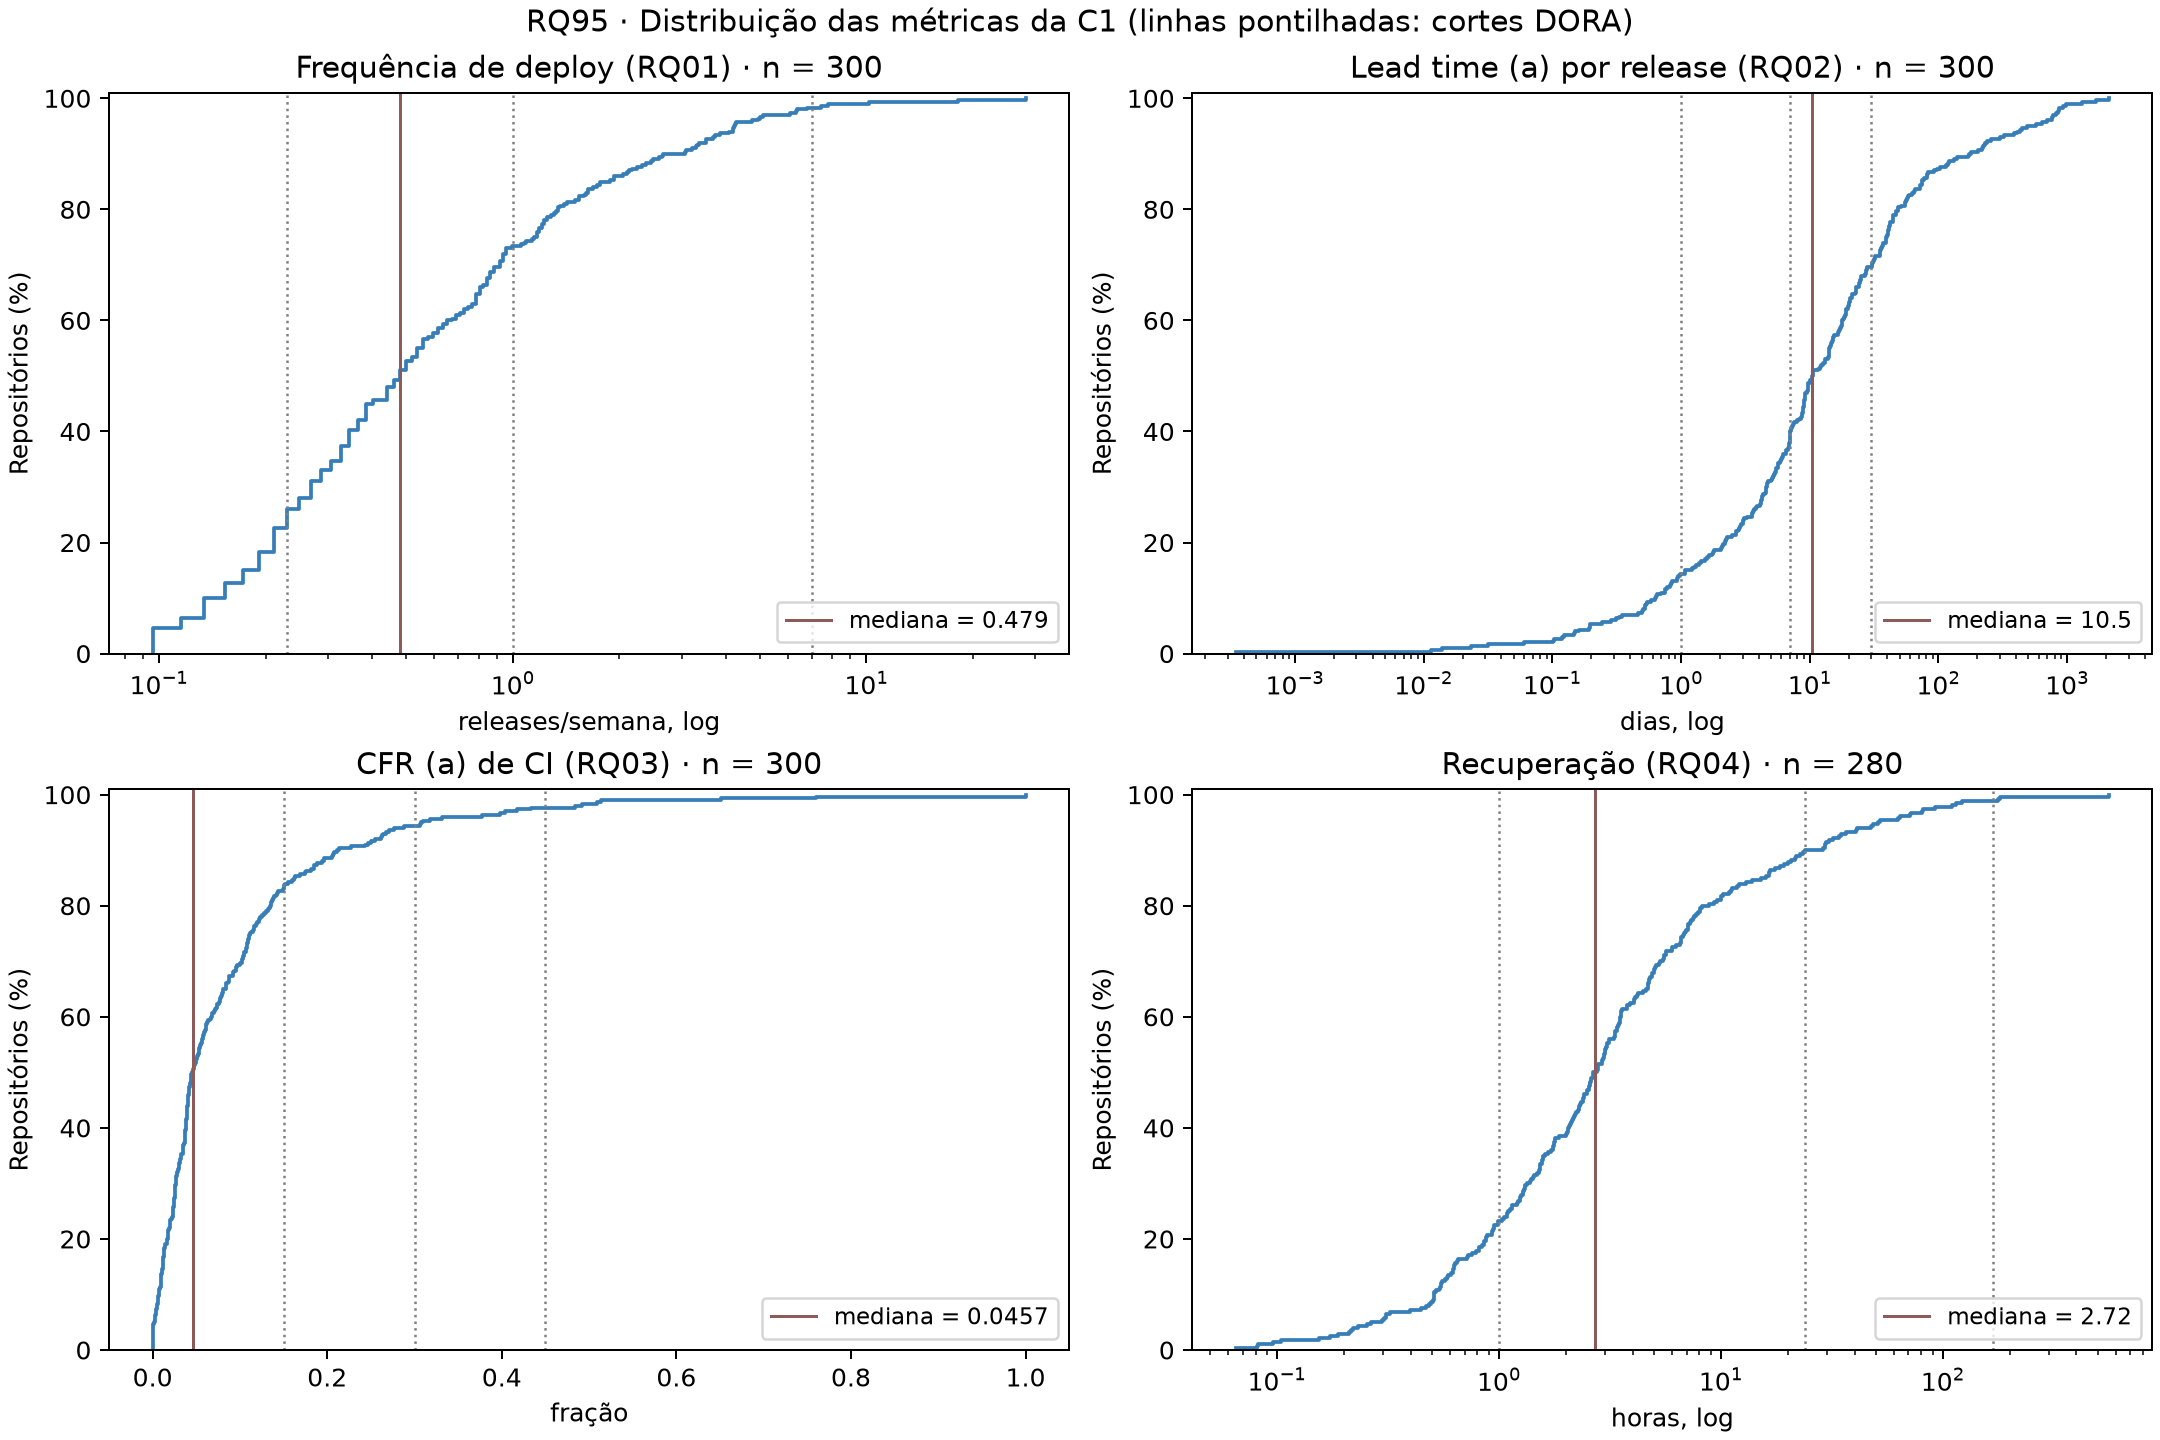
\includegraphics[width=0.92\linewidth]{figuras/distribuicoes_c1.png}
\caption{Distribuição acumulada das métricas da combinação C1 (linhas pontilhadas: cortes DORA;
linha vermelha: mediana).}
\label{fig:distribuicoes}
\end{figure}

\subsection{RQ01 --- Frequência de deploy}

A mediana é de 0,48 release/semana (IQR 0,93), com cauda longa à direita: o máximo é de 28,2
releases/semana e 33 repositórios passam do limite de Tukey (2,54). Os 30 repositórios mais
ativos (10\%) concentram 51,5\% das releases. Metade dos repositórios é Medium (50,7\%), um quarto é
High e só 5 (1,7\%) são Elite.

\subsection{RQ02 --- \textit{Lead time}}

Por release (a), a mediana é de 10,5 dias (IQR 35,9); por \textit{commit} (b), 12,1 dias (IQR 54,3).
Das 18.206 releases da janela, 14.589 têm \textit{lead time}; as demais são a primeira release
da história do repositório (57) ou não trazem \textit{commits} novos (3.560). A variante (b) é
menor que a (a) em 177 repositórios e maior em 122; a razão (b)/(a) tem mediana de 0,78 e o
teste de Wilcoxon pareado não rejeita a igualdade ($p = 0{,}12$). Trocar (a) por (b) muda a classe de
127 repositórios (42,3\%). Quanto maior a release, menor o (b) em relação ao (a)
($\rho = -0{,}30$ entre o número de \textit{commits} por release e a razão (b)/(a)).

\subsection{RQ03 --- Taxa de falha das mudanças}
\label{sec:rq03}

O CFR de CI (a) tem mediana de 4,6\% (IQR 8,8 pontos percentuais): 83,0\% dos repositórios são
Elite, e só 14 não têm nenhuma falha. O CFR de entrega (b), com a v1, tem mediana de 18,8\%
(IQR 44,7 pontos), muito mais disperso, e espalha os repositórios pelas quatro classes
(Tabela~\ref{tab:descritivo}). Somando todos os \textit{runs} e todas as releases, o CFR é de
9,2\% (a) e de 38,2\% (b). As duas variantes quase não concordam: $\rho = 0{,}07$ entre elas
($p = 0{,}26$), o (b) é maior que o (a) em 182 de 299 repositórios (Wilcoxon, $p < 10^{-15}$)
e 57,2\% dos repositórios mudam de classe ao trocar uma pela outra
($\kappa$ ponderado $= 0{,}02$, concordância leve), 144 deles para pior.

Os dois proxies medem coisas diferentes. No (a), 98,6\% das falhas são \texttt{failure} e 1,4\%
são \texttt{startup\_failure}, e o workflow que mais falha em cada repositório responde, na
mediana, por 73,1\% das falhas: o CFR (a) reflete sobretudo um ou dois \textit{workflows}. No
(b), 39,2\% das releases (7.130 de 18.206) têm tag fora do SemVer estrito e nunca são
corretivas na v1; 42 repositórios não têm nenhuma tag SemVer, e o CFR (b) deles é zero por
construção. Por outro lado, na mediana 42,9\% das releases de um repositório mudam só o
\textit{patch}. O nível do (b) depende da heurística: com as versões v2 (\textit{patch} ou qualquer
\textit{commit} com \texttt{fix}, \texttt{revert} ou \texttt{hotfix}) e v3 (correção de defeito),
a mediana vai a 43,5\% e 27,3\%, e 40,8\% e 31,8\% dos repositórios mudam de classe em relação à
v1. A v2 e a v3 marcam como corretivas 98,6\% e 61,3\% das releases na mediana, o que indica
excesso de marcações.

\begin{figure}[ht]
\centering
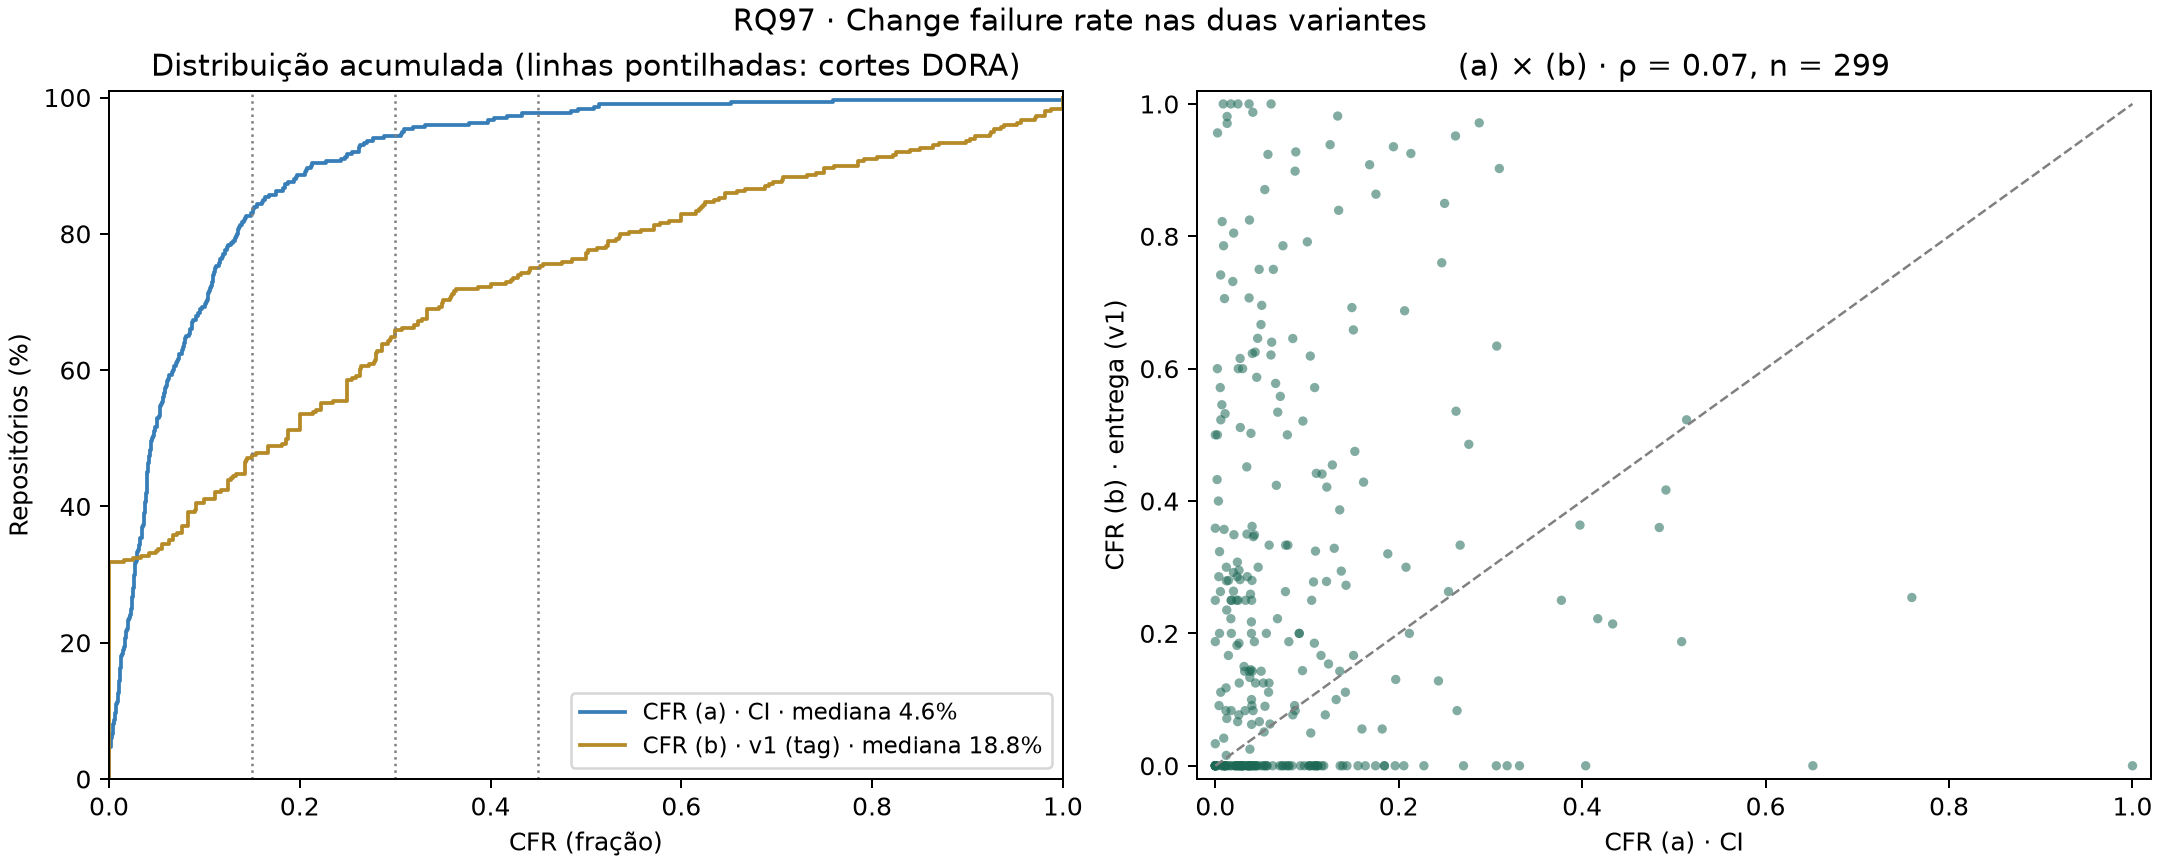
\includegraphics[width=0.95\linewidth]{figuras/cfr_variantes.png}
\caption{CFR nas duas variantes: distribuição acumulada (esquerda) e dispersão (a)~$\times$~(b)
(direita); linha tracejada: $y = x$.}
\label{fig:cfr}
\end{figure}

\subsection{RQ04 --- Tempo de recuperação}

Há 280 repositórios com tempo estimável (20 não têm nenhum episódio de falha completo e ficam
sem estimativa, não com zero). A mediana é de 2,7 horas (IQR 5,7), com cauda longa: o P90 é de
24,5 horas e o máximo, de 560 horas. Dos 27.839 episódios, 230 (0,83\%) terminam censurados à
direita, mas 24 repositórios têm pelo menos 10\% dos episódios censurados. Em 88,9\% dos
episódios a recuperação ocorre em até 24 horas (79,2\% com peso igual por repositório).

\subsection{Classificação DORA geral}

Pela combinação de referência C1 (release, \textit{lead time} (a), CFR (a)), 280 repositórios
recebem classe geral: 6,4\% Elite, 43,6\% High, 45,7\% Medium e 4,3\% Low; os 20 repositórios sem
episódio de falha completo ficam sem classe. A estabilidade é alta (Elite ou High nas duas métricas
da dimensão) em 85,4\% dos repositórios classificados, mas só 21,1\% têm velocidade alta. A classe
geral é limitada pela velocidade, não pela estabilidade.

\subsection{RQ05 --- Frequência de deploy e CFR}
\label{sec:rq05}

\begin{table}[ht]
\centering
\small
\caption{Correlação de Spearman entre a frequência de deploy e o CFR (IC de 95\% por
\textit{bootstrap}; $p$ com correção de Holm). O $\rho$ parcial controla idade e contribuidores
no (a) e o CFR (b) esperado ao acaso no (b) (Seção~\ref{sec:discussao}).}
\label{tab:rq05}
\begin{tabular}{lrrrrr}
\hline
Variante & $n$ & $\rho$ & $p$ (Holm) & IC 95\% & $\rho$ parcial \\
\hline
CFR (a), CI           & 300 & 0,15 & 0,009            & 0,04 a 0,27 & 0,09 ($p = 0{,}14$) \\
CFR (b), entrega (v1) & 299 & 0,40 & $2 \times 10^{-12}$ & 0,29 a 0,51 & $-0{,}16$ ($p = 0{,}005$) \\
\hline
\end{tabular}
\end{table}

A frequência de deploy tem correlação fraca e positiva com o CFR (a) e moderada e positiva com o CFR (b)
(Tabela~\ref{tab:rq05}, Figura~\ref{fig:rq05}). Em quartis de frequência, a mediana do CFR (a) fica
em torno de 4--7\% em todas as faixas, enquanto a do CFR (b) sobe de 0\% (Q1) para 44,2\% (Q4).
Em termos de classes, 94\% dos repositórios de frequência alta (Elite ou High) têm CFR (a) Elite
ou High, contra 95\% dos de frequência baixa (Fisher, $p = 0{,}78$); no CFR (b), 40\% contra 75\%
($p < 10^{-7}$).

\begin{figure}[ht]
\centering
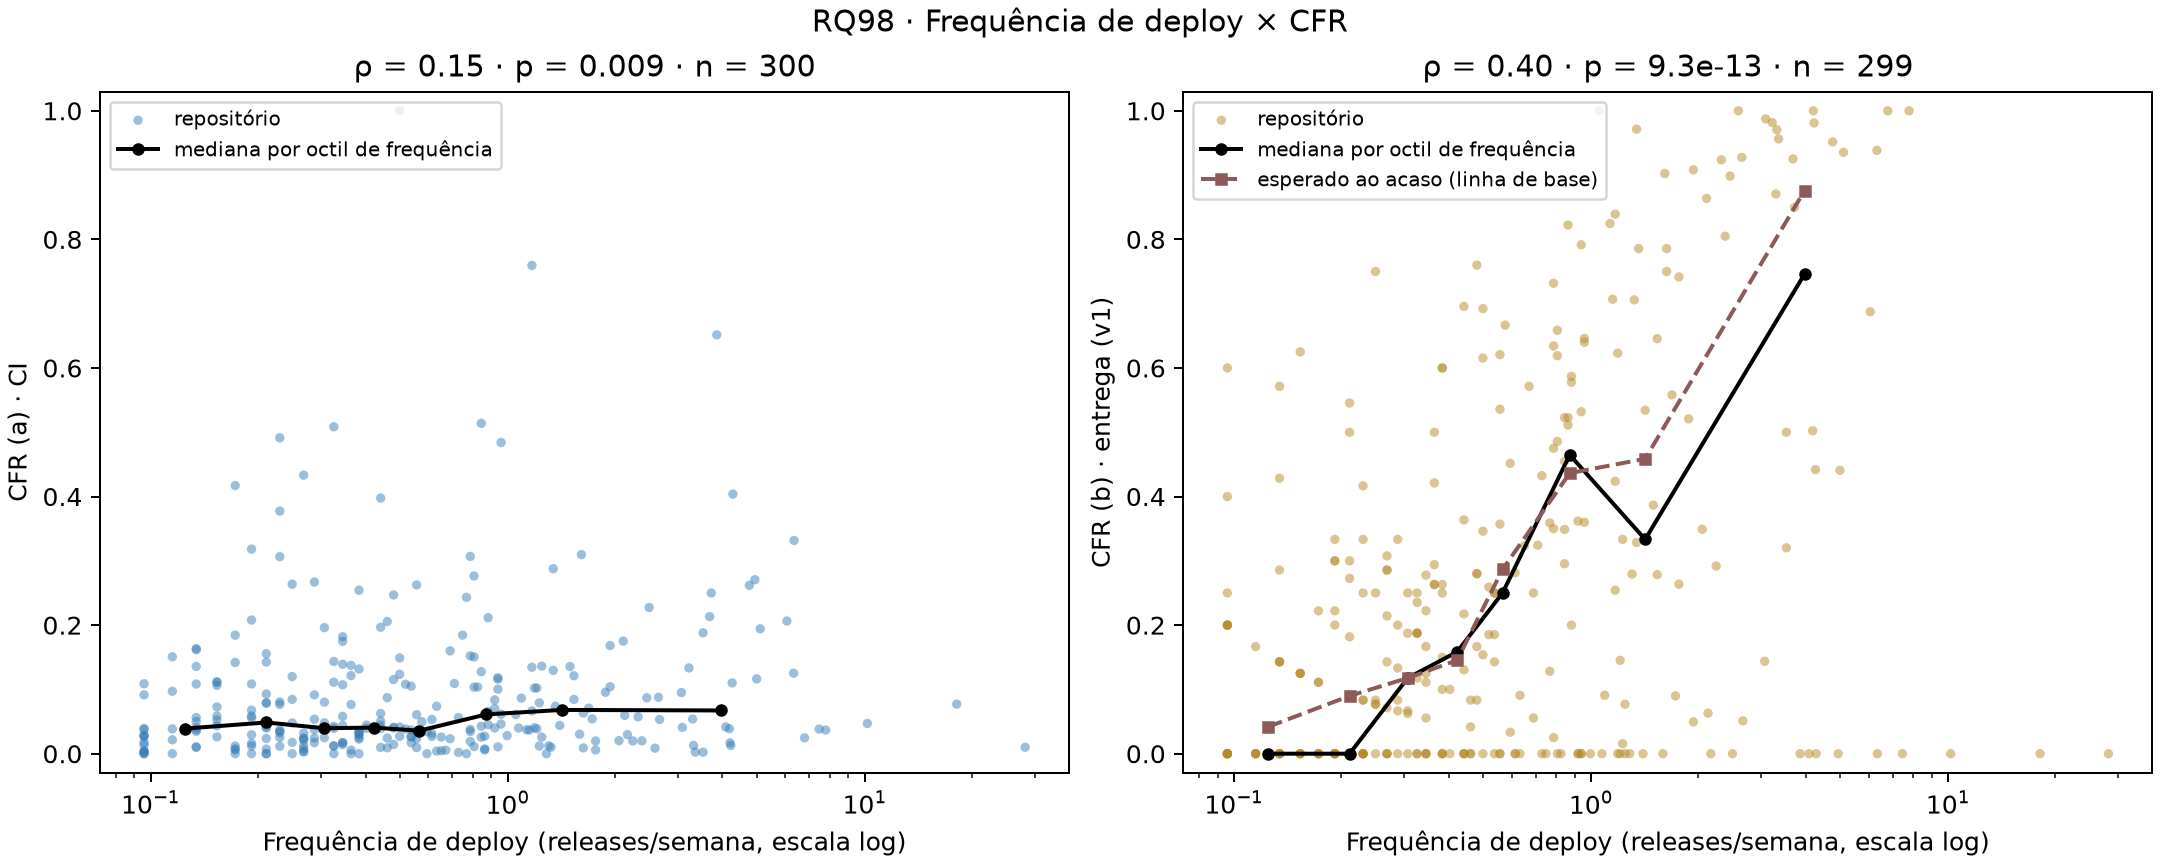
\includegraphics[width=0.95\linewidth]{figuras/dispersao_df_cfr.png}
\caption{Frequência de deploy (escala logarítmica) e CFR. Linha preta: mediana por octil de
frequência; linha tracejada: CFR (b) esperado ao acaso (linha de base da Seção~\ref{sec:discussao}).}
\label{fig:rq05}
\end{figure}

\subsection{RQ06 --- Características dos repositórios}
\label{sec:rq06}

\apreencher{resultados da RQ06 (issue \#93): Kruskal-Wallis ou Mann-Whitney por fator, p-valores
com correção de Holm, $\varepsilon^2$ e $\delta$ de Cliff}

\subsection{RQ07 --- Sensibilidade da classificação DORA}

Classificamos cada repositório em sete combinações de definições (C1 a C7, Tabela~\ref{tab:rq07}).
Dos 279 repositórios classificados em todas elas, 163 (58,4\%) têm a mesma classe geral em todas
e 116 (41,6\%) mudam em pelo menos uma alternativa à C1. Trocar só a unidade de deploy (C5 e C6)
muda de 3,6\% a 10,7\% das classes, sempre para melhor ($\kappa$ de 0,85 a 0,95); as
combinações com o CFR (b) mudam de 20,8\% a 35,5\%, e 75\% das mudanças são para pior. No nível
de cada métrica, trocar o CFR (a) pelo (b) muda a classe de 57,2\% dos repositórios
($\kappa = 0{,}02$), o \textit{lead time} (a) pelo (b), de 42,3\%, e a unidade de deploy de
release para tag, de 24,0\%.

\begin{table}[ht]
\centering
\small
\caption{Mudança da classe geral em relação à C1 (279 a 280 repositórios por par).}
\label{tab:rq07}
\begin{tabular}{llrrl}
\hline
Combinação & O que muda em relação à C1 & Mudam (\%) & $\kappa$ pond. & Landis--Koch \\
\hline
C2 & \textit{lead time} (b)                     & 14,3 & 0,79 & substancial \\
C3 & CFR (b)                                    & 20,8 & 0,68 & substancial \\
C4 & \textit{lead time} (b) e CFR (b)           & 29,7 & 0,52 & moderada \\
C5 & pré-releases contam como deploy            & 3,6  & 0,95 & quase perfeita \\
C6 & tags contam como deploy                    & 10,7 & 0,85 & quase perfeita \\
C7 & tags, \textit{lead time} (b) e CFR (b)     & 35,5 & 0,44 & moderada \\
\hline
\end{tabular}
\end{table}
.
% Os numeros vem das mesmas analises da Secao 3 (entregas/laboratorio-03/sprint-03, RQ91 a RQ98).
% Trechos em \apreencher{...} dependem da RQ06 (issue #93) e da validacao manual (issues #85 a #89).

\providecommand{\apreencher}[1]{\textbf{[a preencher: #1]}}

\section{Discussão}
\label{sec:discussao}

\subsection{Hipóteses e resultados}

A Tabela~\ref{tab:hipoteses} confronta cada hipótese informal da Seção~\ref{sec:hipoteses},
registrada antes da análise, com o que encontramos. Nenhuma faixa prevista foi alterada depois
da análise.

\begin{table}[ht]
\centering
\scriptsize
\caption{Hipóteses (Seção~\ref{sec:hipoteses}) frente aos resultados (Seção~\ref{sec:resultados}).}
\label{tab:hipoteses}
\begin{tabular}{p{0.05\linewidth}p{0.28\linewidth}p{0.40\linewidth}p{0.15\linewidth}}
\hline
 & Previsão & Resultado & Veredito \\
\hline
H1 & Mediana de 0,5 a 1 release/semana; Medium e High; cauda longa; poucos Elite
   & Mediana de 0,48; Medium e High somam 75,7\%; 33 extremos; 1,7\% Elite
   & Confirmada, com a mediana pouco abaixo da faixa \\
H2 & (a) em semanas (Medium ou Low); (b) sistematicamente menor; diferença cresce com o tamanho da release
   & (a) = 10,5 dias, com 60,7\% em Medium ou Low; (b) = 12,1 dias, menor em 177 de 300 repositórios, mas
     sem diferença pareada ($p = 0{,}12$); $\rho = -0{,}30$ com o tamanho
   & Parcial: (a) e o efeito do tamanho sim; (b) menor, não \\
H3 & CFR (a) de 10 a 25\%; (b) de 5 a 15\% e mais variável; $|\rho| < 0{,}3$ entre (a) e (b)
   & (a) = 4,6\%; (b) = 18,8\%, com IQR de 44,7 contra 8,8 pontos; $\rho = 0{,}07$
   & Parcial (2 de 4): variabilidade e correlação sim; níveis, não \\
H4 & Recuperação de 1 hora a 1 dia; cauda longa; censura abaixo de 10\%
   & 2,7 horas; P90 de 24,5 horas e máximo de 560; censura de 0,83\% (24 repositórios com $\geq 10$\%)
   & Confirmada \\
H5 & $\rho$ próximo de zero ou levemente negativo no (b) e próximo de zero no (a)
   & (a) $\rho = 0{,}15$; (b) $\rho = 0{,}40$, ou $-0{,}16$ após a linha de base
   & Parcial: vale, fracamente, no (a); não vale no (b) bruto \\
H6 & Efeitos pequenos a médios; contribuidores, tipo e linguagem associados
   & \apreencher{RQ06 (issue \#93)}
   & Pendente \\
H7 & $\geq 30$\% mudam de classe; $\kappa$ de 0,2 a 0,6; pré-releases e tags inflam a frequência; \textit{lead time} (b) melhora a classe
   & 1 de 6 alternativas com $\geq 30$\% (C7: 35,5\%); $\kappa$ de 0,44 a 0,95; pré-releases e tags só melhoram a classe de frequência; (b) melhora 61 repositórios e piora 66
   & Parcial: depende de qual definição muda \\
\hline
\end{tabular}
\end{table}

\subsection{O que surpreendeu e por quê}

\textbf{A velocidade é o gargalo; a estabilidade quase nunca.} Esperávamos CFR de CI entre 10\% e
25\% e encontramos 4,6\%. Com o corte de Elite em 15\%, 83\% dos repositórios são Elite no CFR (a),
e 85,4\% têm estabilidade alta contra 21,1\% com velocidade alta. O resultado é coerente com o
perfil da amostra, projetos populares com CI madura, mas também com a natureza do proxy: o CFR (a)
mede falha de pipeline, concentrada em um ou dois \textit{workflows} (73,1\% das falhas, na mediana),
e não mede defeito que chega ao usuário. Os cortes DORA vêm de questionários com empresas; aqui o
CFR (a) discrimina pouco, e a classe geral fica presa à frequência e ao \textit{lead time}. Já a
frequência baixa tem uma leitura própria: uma biblioteca que publica uma release por mês não está
``deployando'' nada, e a classe Medium da maioria dos repositórios reflete o ritmo de publicação,
não necessariamente uma entrega lenta.

\textbf{Os dois CFR respondem a perguntas diferentes.} O CFR (b) não ficou abaixo do (a), como
previsto, e a correlação entre eles é desprezível ($\rho = 0{,}07$); 57,2\% dos repositórios mudam de
classe ao trocar um pelo outro. A previsão de que medem fenômenos distintos se confirmou, mas o
nível do (b) é frágil: depende de uma heurística cuja versão v1 deixa de fora 39,2\% das releases
(tags fora do SemVer), e a mediana vai de 18,8\% a 43,5\% conforme a versão
(Seção~\ref{sec:rq03}). Sem o F1 contra o consenso da amostra-ouro (\apreencher{P, R e F1 das versões
da heurística e $\kappa$ de Fleiss entre os avaliadores}), não sabemos qual dessas taxas se aproxima da
taxa real de releases corretivas; por isso reportamos as duas variantes e não escolhemos a mais
favorável a uma hipótese.

\textbf{Mais releases, mais CFR (b), mas por aritmética.} Esperávamos ausência de \textit{trade-off}, em
linha com o DORA. O $\rho$ bruto entre frequência e CFR (b) foi de $0{,}40$, e 40\% dos repositórios de
frequência alta têm CFR (b) Elite ou High, contra 75\% dos de frequência baixa. Lido sem cuidado, isso
sugeriria que publicar mais piora a estabilidade. Mas o CFR (b) conta uma falha quando alguma release
\textit{patch} sai em até 7 dias, e quanto mais releases, maior a chance de isso acontecer ao acaso: a fração
de releases com alguma sucessora em 7 dias tem $\rho = 0{,}83$ com a frequência, enquanto a proporção de
\textit{patches} quase não varia com ela. Embaralhando, em cada repositório, quais releases são corretivas,
o CFR (b) esperado ao acaso tem $\rho = 0{,}59$ com a frequência, acima do observado, e o $\rho$ parcial,
controlando esse esperado, é $-0{,}16$. Para o CFR (a), a relação é fraca ($\rho = 0{,}15$) e perde a
significância ao controlar idade e contribuidores ($0{,}09$; $p = 0{,}14$). Assim, os dados
\textit{open source} não confirmam nem contradizem a afirmação do DORA de que velocidade e estabilidade
andam juntas: o proxy de entrega tem um acoplamento aritmético com a frequência, e o de CI quase não
discrimina. Correlação não implica causalidade; tamanho da equipe, maturidade e automação de
releases podem afetar as duas medidas.

\textbf{\textit{Lead time} por \textit{commit} não é menor que por release.} Previmos o (b) sistematicamente
menor, porque um \textit{commit} antigo ``esquecido'' infla o (a) e é diluído no (b). O mecanismo aparece nas
releases grandes ($\rho = -0{,}30$ entre o tamanho e a razão (b)/(a)), mas o (b) pondera as releases pelo
número de \textit{commits}: onde poucas releases grandes concentram \textit{commits} antigos e muitas releases
pequenas são rápidas, a mediana por \textit{commit} cai dentro das grandes e supera a por release. No
agregado, as variantes divergem em ambos os sentidos, e o teste pareado não as separa.

\textbf{A classificação é frágil, mas não a todas as escolhas.} Dos repositórios classificados em todas as
combinações, 41,6\% mudam de classe em pelo menos uma alternativa, e o efeito não é uniforme: trocar a
unidade de deploy muda de 3,6\% a 10,7\% das classes, sempre para melhor ($\kappa \geq 0{,}85$), enquanto as
combinações com o CFR (b) mudam de 20,8\% a 35,5\%, em geral para pior ($\kappa$ de 0,44 a 0,68). Como o CFR (b) depende de uma heurística
ainda sem F1, parte desse efeito pode ser do proxy, não da definição. As conclusões das RQ01 a RQ05
valem, portanto, para a combinação C1 e são condicionais à definição de falha, e menos à de deploy.

\subsection{Implicações}

Para quem minera métricas DORA no GitHub, três cuidados decorrem dos resultados. Primeiro, release
não é deploy, e falha de CI não é falha em produção; as classes servem para comparar repositórios entre si,
não para dizer que um projeto de código aberto é ``Elite'' no sentido do DORA. Segundo, o CFR
baseado em releases corretivas só tem sentido com uma heurística validada contra julgamento humano, e
deve ser comparado ao que o acaso produziria quando a frequência de releases é alta. Terceiro, vale
reportar a sensibilidade às definições, como fizemos na RQ07, porque a escolha do CFR por si só
reclassifica de 20,8\% a 35,5\% dos repositórios. A RQ06 (características dos repositórios)
ainda não foi analisada (\apreencher{discussão da RQ06 e da H6}); as ameaças à validade que decorrem
destes achados estão na Seção~5.
